\chapter[Optoelectronic Properties of Heterostructure Bilayers]{Electronic and Optical Properties of 2D Heterostructure Bilayers of Graphene, Borophene and 2D Boron Carbides from First-Principles}
\label{cha:project_1}

\section{Abstract}

In the present work, 
the atomic, electronic, and optical properties of two-dimensional graphene, borophene, and boron carbide heterojunction bilayer systems (\ce{Graphene-BC3}, \ce{Graphene-Borophene}, and \ce{Graphene-B4C3}),
as well as their constituent monolayers are investigated on the basis of first-principles calculations using the HSE06 hybrid functional.
Our calculations show that while borophene is metallic,
both monolayer \ce{BC3} and \ce{B4C3} are indirect semiconductors,
with band gaps of $1.822$ eV and $2.381$ eV as obtained using HSE06.
The \ce{Graphene-BC3} and \ce{Graphene-B4C3} bilayer heterojunction systems maintain the Dirac point of graphene at the $\vec{k}$-point and are semi-metals,
while \ce{Graphene-Borophene} is metallic.
All bilayer heterostructure systems possess absorbance in the visible region where the resonance frequency and resonance absorption peak intensity vary between structures.
Remarkably, all heterojunctions support plasmons within the range $16.5-18.5$ eV, while \ce{Graphene-B4C3} and \ce{Graphene-Borophene} exhibit a $\pi$-type plasmon within the region 4-6 eV,
with the latter possessing an additional plasmon at the lower energy of $1.5-3$ eV.
The dielectric tensor for \ce{Graphene-B4C3} exhibits complex off-diagonal elements due to the lower P3 space group symmetry indicating it has anisotropic dielectric properties and could exhibit optically active (chiral) effects.
Our study shows that the two-dimensional heterostructures have desirable optical properties broadening their potential applications.

\newpage
\section{Introduction}

\ce{Graphene} is well-known to have excellent electrical conductivity,
desirable mechanical and thermal properties,
and high light transmittance in the visible light-infrared region.
It also has an extremely high quantum efficiency for light-matter interactions and is strongly optically nonlinear.
It has therefore found applications in e.g. electronics, energy storage, biomedical and other fields~\cite{janavika2023graphene}. 
Relative to conventional plasmonic materials, graphene possesses highly confined plasmons with much longer lifetimes.
Also, graphene plasmons are active in an extended wavelength range, namely, the mid-infrared and terahertz regime.
This wavelength range overlaps with the feature signals of most organic and biomolecules,
which has broadened graphene's applications towards plasmonic biological and chemical sensors~\cite{sakthivel2023} in addition to plasmonic waveguides,
and infrared photodetectors.
Moreover, the properties can be tuned by forming graphene-hybrid materials, finding applications in biosensors, chemical sensors, optical sensors, and other types of sensors~\cite{zhang2022}.

In other areas, however, the use of graphene has been limited due to its zero-value band gap.
One of the methods used to expand the application of graphene is to form heterostructures.
Stacking different two-dimensional (2D) materials together can form double-layer or even multi-layer artificial materials that are maintained by van der Waals interactions~\cite{novoselov20162d}.
Such materials are known as van der Waals heterojunctions.
A wide range of physical properties can be obtained by such stacking,
making van der Waals heterojunctions even more important than the 2D material itself.
There are vast numbers of 2D materials, and with forming heterostructures thereof,
a diverse range of electrical, photonic, plasmonic, mechanical, and chemical properties can be theoretically predicted through {\em ab initio} calculations and machine learning~\cite{thygesen2017,he2023}, and experimentally engineered~\cite{lin2023recent,elbanna20232d}.

Recently, the prospect of developing plasmonic devices employing 2D semiconductors has attracted considerable attention~\cite{agarwal2018plasmonics, qiu2018optical}. 
Plasmonic modes in each class of van der Waals semiconductors have their own peculiarities, along with potential technological capabilities.
Recently, graphene-like \ce{BC3} has been synthesized experimentally~\cite{yanagisawa2004phonon, yanagisawa2006phonon, tanaka2005novel} and is found to be semiconducting with an indirect bandgap.
Calculations have shown that nanostructures of graphene-like \ce{BC3} possess desirable absorbance in the visible region and by changing the size of the nanostructure,
the resonance peak position of the absorption spectrum can be effectively regulated~\cite{chen2019plasmon}.
Recent studies have also predicted a stable \ce{B4C3} monolayer,
which is even more stable than the previously synthesized BC3 monolayer~\cite{tian2019}.
Boron carbides are known for their exceptional hardness, 
thermal stability, and chemical inertness.
The emergence of 2D boron carbides adds a new dimension to the study of these materials,
offering novel properties and opportunities for technological innovation~\cite{luo2011predicting,fan2018two}.

Borophene is another 2D material of high current interest.
This monolayer allotrope of boron forms several structures and is characterized by its unique atomic structure and exceptional electronic properties,
which has opened new avenues for innovation in the areas of electronics,
energy storage, catalysis, plasmonics, superconductivity, and sensors~\cite{qiu2018optical}.
One particularly intriguing aspect of borophene's versatility lies in its ability to form heterojunctions—interfaces between different borophene structures or between borophene and other materials.
Borophene-graphene heterostructures have been realized~\cite{hou2021borophene}, 
where they have shown good stability and ability to function as a humidity sensor,
exhibiting a sensitivity about 700 times higher than that of pristine graphene,
and 27 times higher than that of borophene.
Also, recently, both lateral and vertical integration of borophene with graphene has been achieved~\cite{liu2019borophene},
as has the formation of bi-layer ($\alpha$-phase) borophene on the Ag(111) surface~\cite{liu2022}.

The synergistic combination of graphene's exceptional electrical conductivity,
mechanical strength, and flexibility with boron carbide's high hardness,
thermal stability, and chemical resistance, and with borophene's attractive electronic properties,
hold tremendous potential for a wide range of applications spanning from electronics and optoelectronics to energy storage and sensing.
As research in this field continues to advance,
the development of scalable synthesis methods, the elucidation of structure-property relationships,
and the exploration of novel applications will be key focal points.
To date, there is little known about the physical properties of graphene-based bilayer heterojunctions with borophene and boron-carbide materials.
This motivates the present work to gain an understanding of these heterojunctions
through the study of their electronic and optical properties on the basis of first-principles calculations.
Such understanding is crucial for their future technological application,
where the unique properties of these materials can be harnessed. 

The paper is organised as follows:
In Section~\ref{1_calculation_method}, the calculation method is described,
followed by the Results and Discussion in Section~\ref{1_results}.
Herein, we describe the physical properties of the monolayers and heterostructures, including band structure, density of states, electron density difference distributions,
Schottky barriers and the optical properties.
This is followed by the Conclusion in Section~\ref{1_conclusions}.

\section{Calculation method}
\label{1_calculation_method}

We perform first-principle calculations using density functional theory (DFT) as implemented in the Vienna Ab initio Simulation Package (VASP)~\cite{kresse1993ab, kresse1996efficiency, kresse1996efficient}.
The projector augmented wave (PAW) method pseudopotentials are used to account for the electron-ion interactions~\cite{kresse1999ultrasoft}.
For the structural optimization calculations, we use the generalized gradient approximation (GGA) of Perdew-Burke-Ernzerhof (PBE) as the exchange-correlation functional.
The Becke-Johnson damped D3(BJ) dispersion correction is also included to account for long-range van der Waals (vdW) interactions.
We use a $\Gamma$-centered $\vec{k}$-point sampling mesh of $11 \times 11 \times 1$, except for the smaller graphene unit cell shown in figure~\ref{s1.1}, for which we use a denser mesh of $23 \times 23 \times 1$.
We set the plane-wave energy cutoff to \qty{450}{\electronvolt}.
Electronic convergence criteria are set to \qty{1e-6}{\electronvolt} and systems are allowed to relax until all forces on each atom are below \qty{0.01}{\electronvolt\per\angstrom}.
For smearing at the Fermi level,
we use the Gaussian smearing method implemented in VASP.

For the calculation of electronic properties,
the PBE exchange-correlation functional is known to underestimate band gap energies.
Therefore, we also use the screened hybrid exchange-correlation functional of Heyd, Scuseria, and Ernzerhof (HSE06),
which gives more accurate band gap energies~\cite{sassnick2021electronic, heyd2003hybrid, krukau2006influence}.

All density of states (DOS) calculations use a $\Gamma$-centered $\vec{k}$-point sampling mesh of $33 \times 33 \times 1$,
with smearing at the Fermi level calculated using the Gaussian method and a broadening value of \qty{0.1}{\electronvolt}.
The HSE06 exchange-correlation functional is also used for the calculation of optical properties,
in particular, the frequency-dependent dielectric function with a $\Gamma$-centered $\vec{k}$-point sampling mesh of $17 \times 17 \times 1$ and $65 \times 65 \times 1$.
The complex frequency-dependent dielectric function, $\varepsilon(\omega)$,
is given by equation \ref{complex_dielectric_function_definition},
where $\varepsilon_{1}(\omega)$ and $\varepsilon_{2}(\omega)$ are the real and imaginary parts, respectively, and $\omega$ denotes the photon energy in \unit{\electronvolt}.

We then use the dielectric function to calculate the absorption coefficient,
refractive index, extinction coefficient, reflectivity, and energy-loss spectrum,
following the relations introduced in section~\ref{sec:from_dielectric_function_to_optical_properties}.

The interlayer binding energy $E_{\mathrm{b}}$ follows as:

\begin{equation}
    E_{\mathrm{b}}
    = E_{\mathrm{H}} - E_{\mathrm{BC}/\mathrm{B}} - E_{\mathrm{G}}
\label{interlayer_binding_energy}
\end{equation}

here, $E_{\mathrm{H}}$ denotes the total energy of the heterostructure,
$E_{\mathrm{BC}/\mathrm{B}}$ corresponds to the total energy of the isolated boron-carbide or borophene monolayer,
and $E_{\mathrm{G}}$ denotes the total energy of the isolated graphene monolayer.

Afterwards, the charge density difference, $\Delta \rho(\vec{r}\,)$ takes the form:

\begin{equation}
    \Delta \rho(\vec{r}\,) =
    \rho_{\mathrm{AB}}(\vec{r}\,)
    - \rho_{\mathrm{A}}(\vec{r}\,)
    - \rho_{\mathrm{B}}(\vec{r}\,)
\label{charge_density_difference}
\end{equation}

here, $\rho_{\mathrm{AB}}(\vec{r}\,)$ denotes the total charge density of the heterostructure.
The terms $\rho_{\mathrm{A}}(\vec{r}\,)$ and $\rho_{\mathrm{B}}(\vec{r}\,)$ represent the charge densities of the isolated monolayers forming the heterostructure.

\section{Results and discussion}
\label{1_results}

\subsection{Monolayer properties}

We start by investigating the structural and electronic properties of the three monolayers,
namely \ce{BC3}, \ce{B4C3} and borophene.
The graphene monolayer is also investigated as it always forms one layer of the heterostructure systems.
The optimized structures of \ce{BC3}, \ce{B4C3}, borophene,
and graphene are shown in figure~\ref{fig1.1}.
The monolayer allotrope of borophene has been predicted to have various low-energy structures with the $\beta_{12}$, 
$\chi_{3}$, and $\alpha'$ structures having been synthesised experimentally~\cite{kaneti2021borophene}.
For this study, we chose to investigate the $\alpha'$ structure of borophene,
not only because it has been synthesised experimentally, 
but also because it has been shown to have the most favourable cohesive energy from GGA level \textit{ab initio} calculations~\cite{wu2012two}.

The structural properties and band gap energies of the monolayer systems are shown in Table~\ref{tab:1.1_monolayer}.
For graphene, the lattice constant is calculated to be $a = 2.467$ $\mathring{\mathrm{A}}$,
while those of borophene, \ce{BC3}, and \ce{B4C3} are 5.051 $\mathring{\mathrm{A}}$, 5.169 $\mathring{\mathrm{A}}$, and 4.690 $\mathring{\mathrm{A}}$, respectively.
In agreement with previous calculations, graphene is a semimetal and borophene is metallic,
whereas \ce{BC3} and \ce{B4C3} are indirect semiconductors~\cite{zhang2018strain, nosheen2022first}.
The calculated indirect band gaps of \ce{BC3} and \ce{B4C3} are \qty{1.822}{\electronvolt} (\qty{0.634}{\electronvolt}) and \qty{2.381}{\electronvolt} (\qty{1.647}{\electronvolt}), respectively, as obtained using HSE06 (PBE).

Figure~\ref{S1.2} shows the optimization of the lattice constants for the monolayers,
while figure~\ref{fig1.2_monolayers_bs} presents the band structures of the four monolayer systems.

\begin{figure}[!htbp]
    \centering
    \includegraphics[width=0.80\textwidth]{figures_proj1/proj1.1.pdf}
    \caption{Optimized atomic structures of \ce{BC3}, borophene, \ce{B4C3}, and graphene.
    Boron and carbon atoms are denoted by the green and brown spheres, respectively.
    Borophene has three unique bonds indicated by $l_1$, $l_2$ and $l_3$,
    while \ce{B4C3} has four unique bonds indicated by $l_4$, $l_5$, $l_6$ and $l_7$.
    The unit cells are highlighted in orange.}
    \label{fig1.1}
\end{figure}

\begin{table}[!htbp]
\centering
\rowcolors{2}{gray!15}{white}
\begin{adjustbox}{max width=1.0\linewidth}
\begin{tabular}{ccm{48px}m{48px}m{48px}m{72px}m{72px}c}
\hline
\rowcolor{gray!25}
system
& $a$ $(a=b)$ (Å) & B-B (Å) & C-C (Å) & B-C (Å) & $E_{\mathrm{g-PBE}}$ (eV) & $E_{\mathrm{g-HSE06}}$ (eV) & Nature \\ \hline
\ce{BC3}
& 5.169 & - & 1.421 & 1.563
& 0.634
\newline (0.62--0.66) 
\newline\cite{behzad2017mechanical,zhang2018theoretical,zhang2018strain}
& 1.822 \newline(1.83)\cite{zhang2018theoretical}
& indirect \\

\ce{Borophene}
& 5.051
& 1.689 ($l_1$) \newline
  1.672 ($l_2$) \newline
  1.707 ($l_3$)
& - & - & - & -
& metallic \\

\ce{B4C3}
& 4.690 & 1.689 ($l_4$) & -
& 1.592 ($l_5$) \newline
  1.517 ($l_6$) \newline
  1.548 ($l_7$)
& 1.647 & 2.381 \newline(2.39)\cite{chang2019b4c3}
& indirect \\

\ce{Graphene}
& 2.467 & - & 1.424 & - & - & - & semimetal \\
\hline
\end{tabular}
\end{adjustbox}

\caption{Optimized lattice constants, inter-atomic distances, and band gaps of monolayer \ce{BC3}, borophene, \ce{B4C3}, and graphene.
Here, $a$ is the lattice parameter with $a=b$ for all systems, B-B, C-C,
and B-C are the boron-boron, carbon-carbon, and boron-carbon bond lengths. 
Borophene and \ce{B4C3} have B-B and B-C bonds of different lengths,
these are identified by labels $l_1,\cdots,l_7$ in figure~\ref{fig1.1}.
The band gap $E_{\mathrm{g}}$ is calculated using the PBE and HSE06 exchange-correlation functionals;
values in brackets are from previous theoretical studies. ``Nature'' indicates the electronic character of the system.}
\label{tab:1.1_monolayer}
\end{table}

\begin{figure}[!htbp]
    \centering
    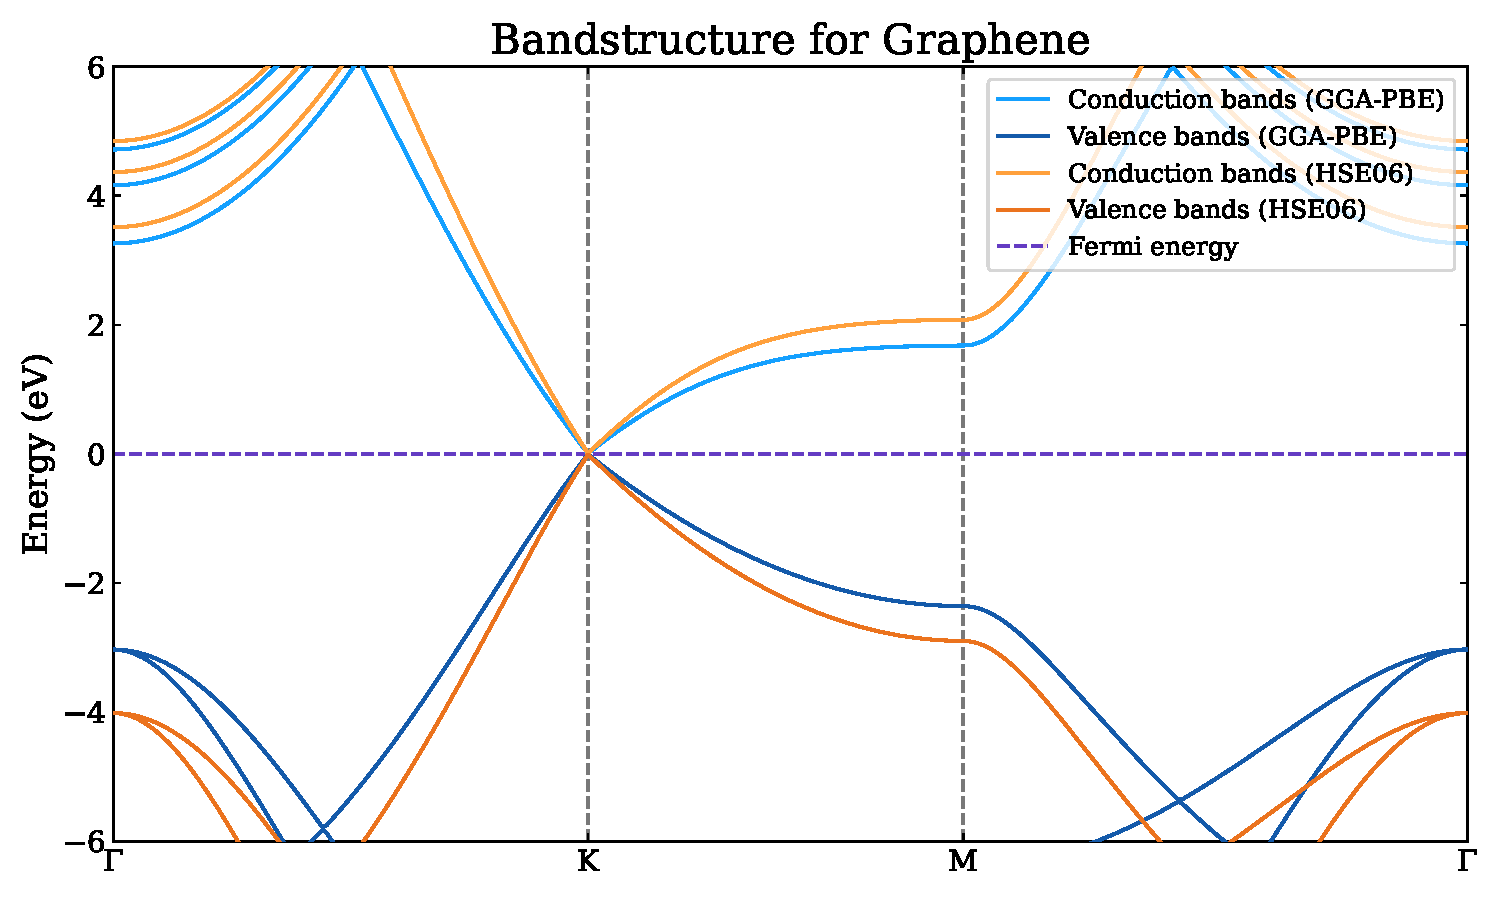
\includegraphics[width=0.40\linewidth]{figures_proj1/proj1.3a.pdf}%
    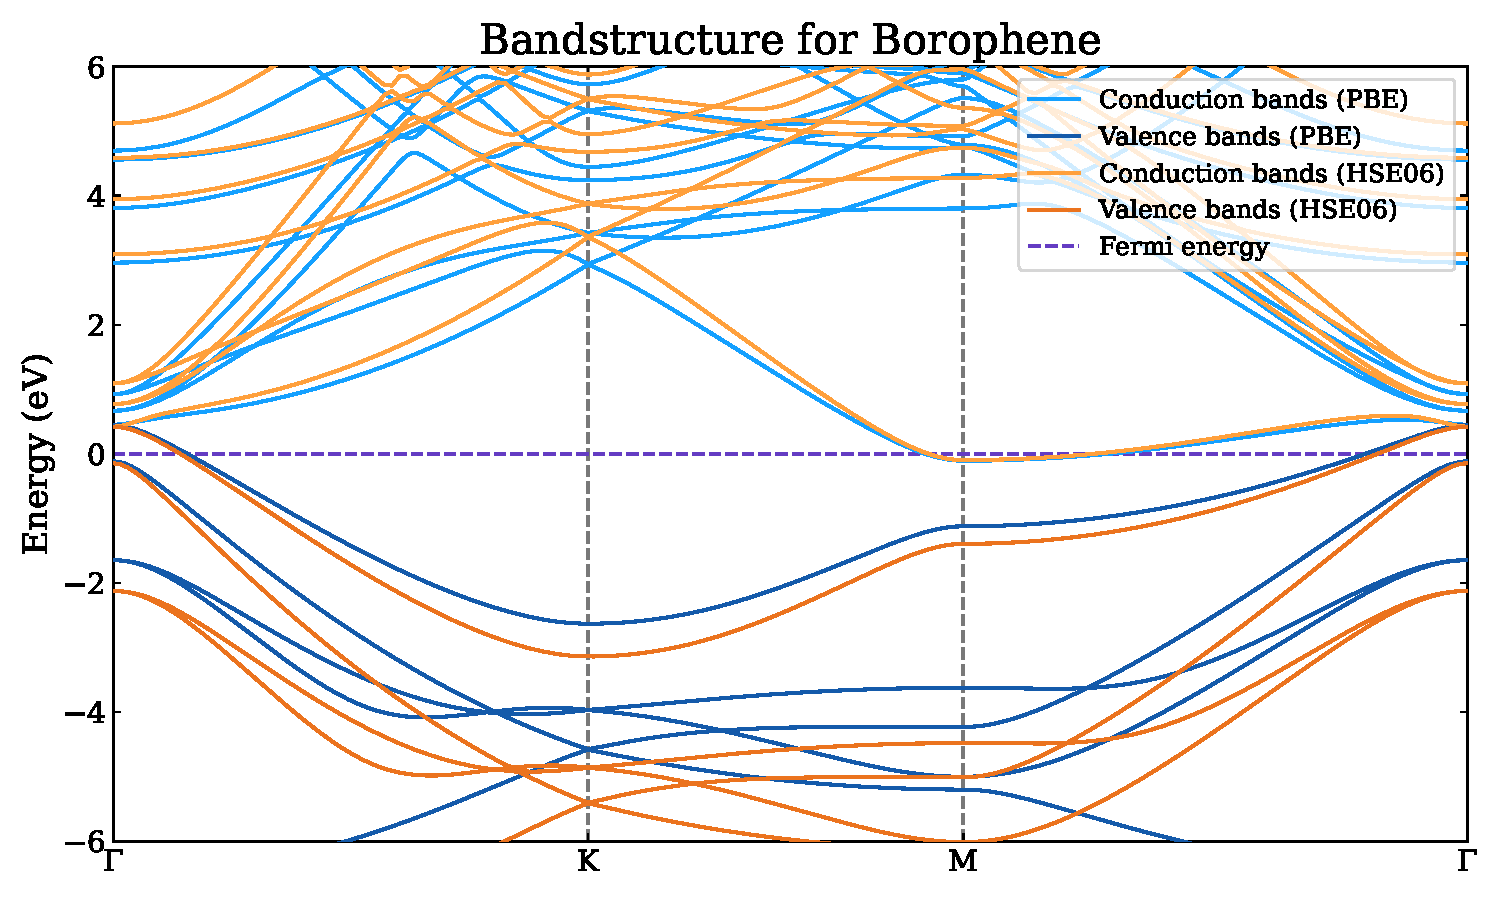
\includegraphics[width=0.40\linewidth]{figures_proj1/proj1.3b.pdf}%
    \par\nointerlineskip
    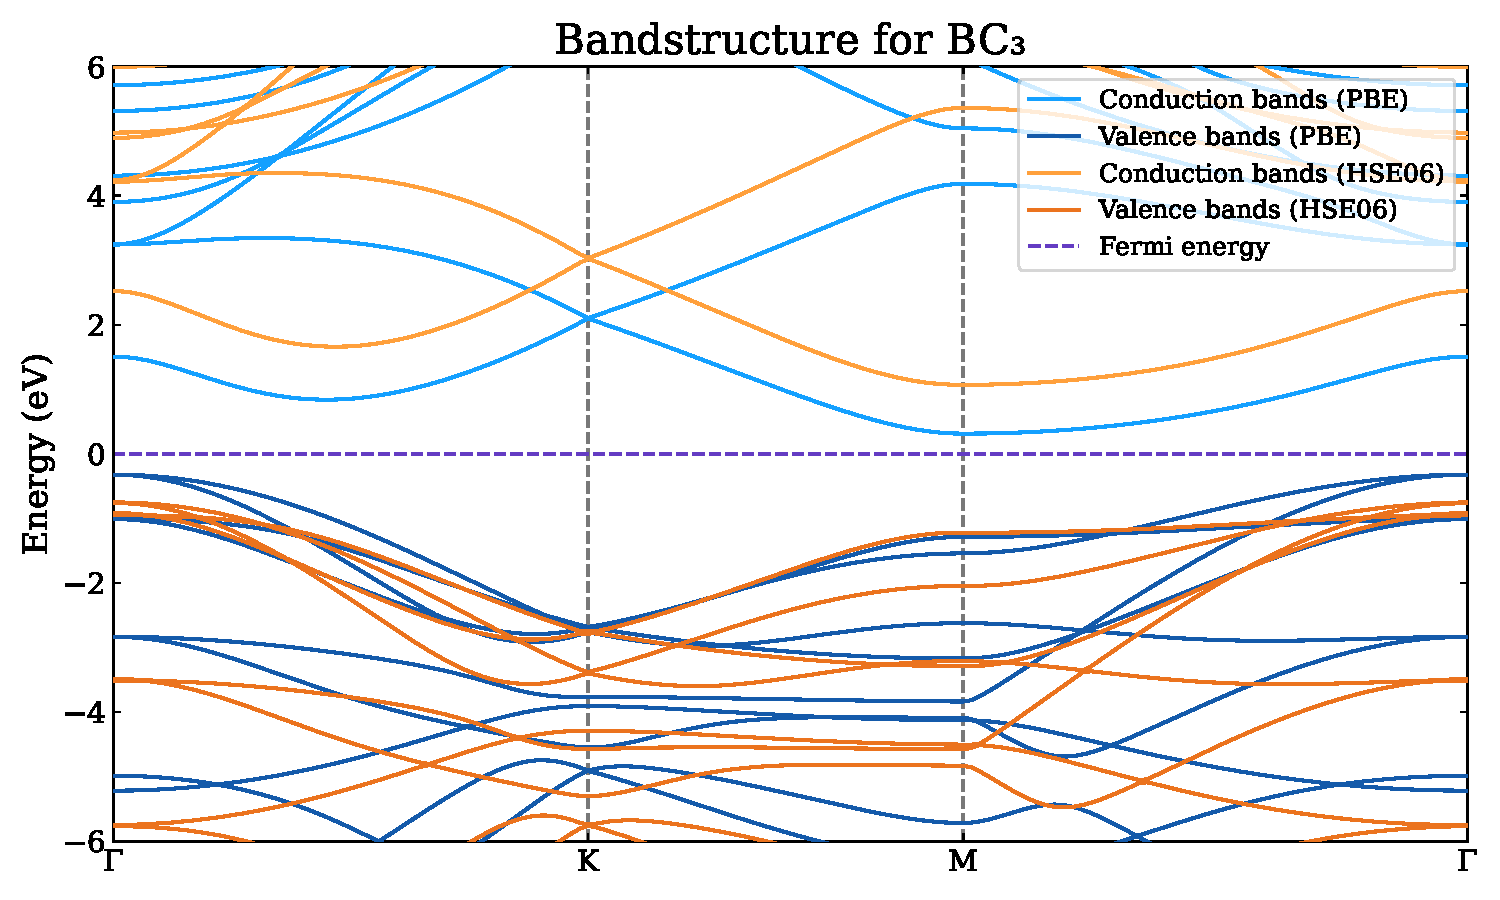
\includegraphics[width=0.40\linewidth]{figures_proj1/proj1.3c.pdf}%
    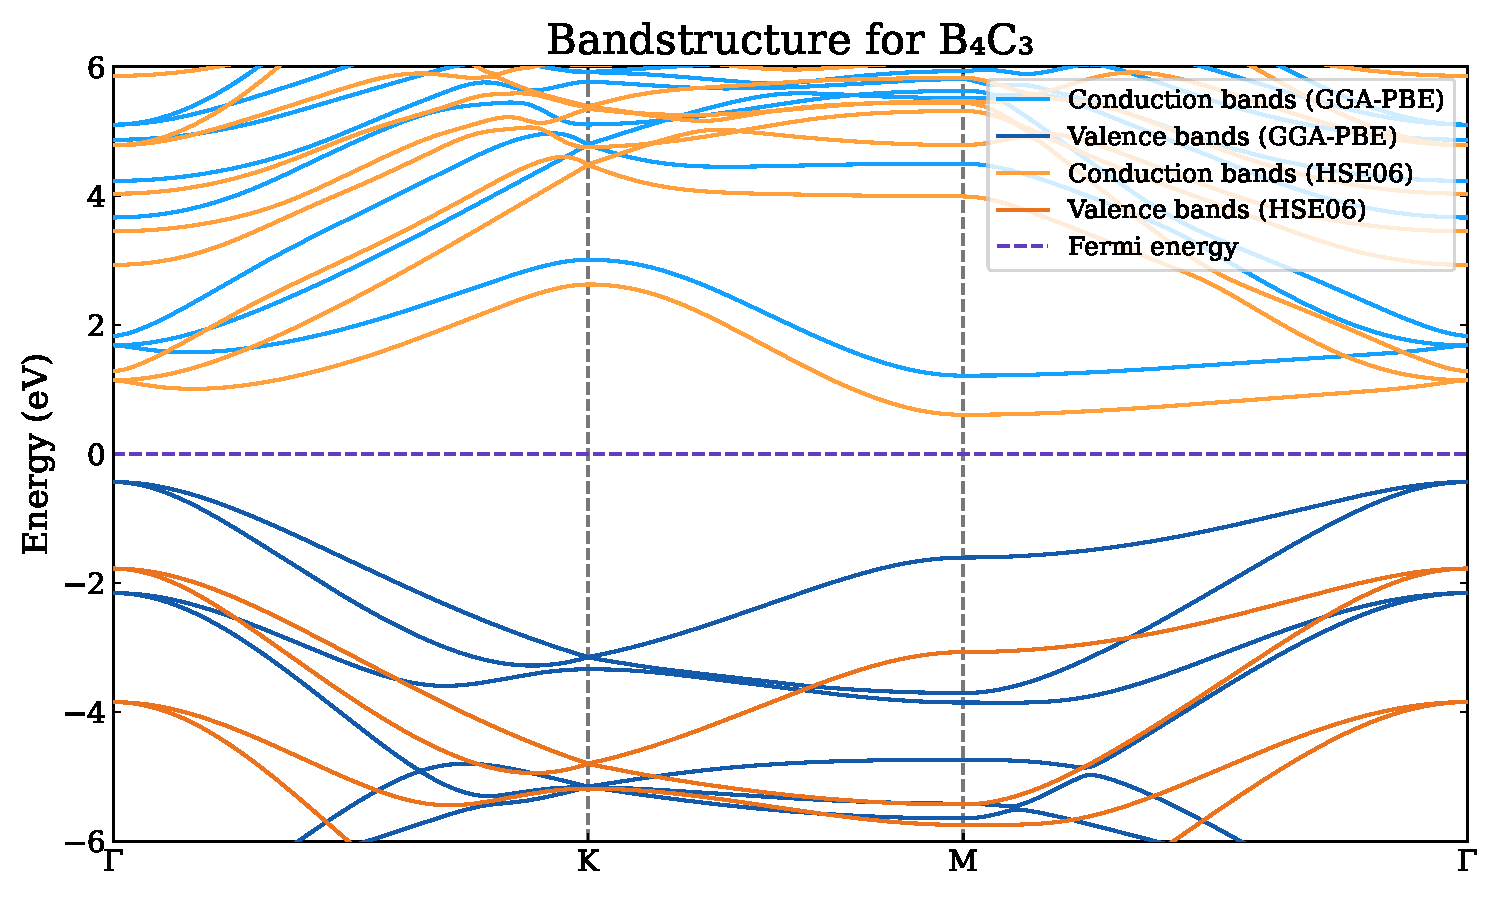
\includegraphics[width=0.40\linewidth]{figures_proj1/proj1.3d.pdf}%
    \caption{Band structures of the four monolayer systems, graphene, borophene, \ce{BC3}, and \ce{B4C3}, calculated using PBE (blue) and HSE06 (orange).}
    \label{fig1.2_monolayers_bs}
\end{figure}

\subsection{Heterostructure}

\subsubsection{Structural properties}

We now turn to determine the structure of the bilayer heterojunctions,
which are composed of monolayer graphene stacked with monolayer \ce{BC3}, borophene,
and \ce{B4C3} (namely, \ce{Graphene-BC3}, \ce{Graphene-Borophene}, and \ce{Graphene-B4C3}), respectively.
To create the heterostructures, we use a ($2\times2\time1$) cell.
For each system,
we considered various lateral coordinations (positions) of these layers.
Specifically, ``Hollow'', ``Bridge'', and ``Top'' coordinations for the \ce{Graphene-BC3} bilayer systems,
and ``Hollow 1'', ``Hollow 2'', ``Bridge'' and ``Top'' coordinations for the \ce{Graphene-Borohene} and \ce{Graphene-B4C3} bilayer systems.
We studied the relative energies,
optimized lattice constants, and inter-planar distances for all structures.
Details about this procedure are given in figures S4-S7.
Due to the weak van der Waals interaction between the layers,
the difference in energies of the lateral positions is very small,
with the values given in figure S8.

The results demonstrate that the energetically most favorable lateral position for the \ce{Graphene-BC3} system is the ``Hollow'' coordination stacking configuration.
As shown in figure~\ref{fig1.3},
this means that each atom in \ce{BC3} is projected onto the center of a hexagon in graphene.
Both the \ce{Graphene-Borophene} and \ce{Graphene-B4C3} bilayer systems energetically favor the ``Top'' coordination stacking configuration.
In this arrangement, each atom-free hexagon in the bottom layer is projected onto the center of a hexagon in graphene.
However, the converse does not hold, as not every hexagon center in graphene aligns with an atom-free hexagon in the bottom layer, as illustrated in figure~\ref{fig1.3}.

\begin{figure}[!htbp]
    \centering
    \includegraphics[width=1.00\textwidth]{figures_proj1/proj1.3.pdf}
    \caption{Top view of the optimized atomic structures of \ce{Graphene-BC3}, \ce{Graphene-Borophene}, and \ce{Graphene-B4C3}.
    Boron and carbon atoms are denoted by the green and brown spheres, respectively.
    The unit cell is indicated by the orange parallelogram.}
    \label{fig1.3}
\end{figure}

\begin{table}[!htbp]
\centering
\rowcolors{2}{gray!15}{white}
\begin{adjustbox}{max width=1.0\linewidth}
\begin{tabular}{ccm{72px}m{64px}m{88px}m{72px}c}
\hline
\rowcolor{gray!25}
system
& coordination
& $a$ $(a=b)$ (Å)
& $S_{\mathrm{G}}$
& $S_{\mathrm{BC}/\mathrm{B}}$
& $d_{\mathrm{IL}}$ (Å)
& Nature \\ \hline

\ce{Graphene-BC3}
& Hollow
& 5.044
& \qty{2.23}{\percent}
& \qty{-2.42}{\percent}
& 3.372
& semimetal \\

\ce{Graphene-Borophene}
& Top
& 4.979
& \qty{0.91}{\percent}
& \qty{-1.43}{\percent}
& 3.505
& metallic \\

\ce{Graphene-B4C3}
& Top
& 4.846
& \qty{-1.78}{\percent}
& \qty{3.33}{\percent}
& 3.514
& semimetal
\\ \hline
\end{tabular}
\end{adjustbox}
\caption{Optimized structural properties for each bilayer heterojunction system,
including the lowest-energy lateral stacking coordination relative to graphene,
the optimized lattice constant $a$,
the strains relative to the respective monolayers, $S_{\mathrm{G}}$ and $S_{\mathrm{BC}/B}$,
the interplanar distance $d_{\mathrm{IL}}$,
and the electronic nature.
Negative and positive percentage strains correspond to compressive and tensile strains, respectively.}
\label{tab:1.2_heterostructure}
\end{table}

It can be seen from table~\ref{tab:1.2_heterostructure} that \ce{Graphene-Borophene} is metallic, 
while  \ce{Graphene-BC3} and \ce{Graphene-B4C3} are semi-metals.
Out of all the heterostructure systems, a maximum (tensile) strain of \qty{3.33}{\percent} is present for \ce{B4C3}.
For the bilayer system \ce{Graphene-BC3}, 
graphene is under tensile strain and \ce{BC3} is under compressive strain.
For the bilayer system \ce{Graphene-Borophene},
a slight tensile strain is present for \ce{Graphene},
while borophene experiences compressive strain.
For the bilayer system \ce{Graphene-B4C3},
there is compressive strain in \ce{Graphene},
while \ce{B4C3} is under a larger tensile strain.
Generally, tensile strain tends to narrow the band gap,
reducing it and increasing conductivity~\cite{roldan2015strain}. 
Conversely, compressive strain tends to widen the band gap, thereby decreasing conductivity~\cite{boukhvalov2008hydrogen}.

\subsubsection{Charge density difference}

The charge density difference distributions for the heterostructure systems are shown in figure~\ref{fig1.4_cdd}.
We calculate these distributions using equation~\ref{charge_density_difference}.
Specifically, we subtract the charge densities of the isolated monolayers from the charge density of the corresponding heterostructure.

\begin{figure}[!htbp]
    \centering
    \includegraphics[width=1.0\textwidth]{figures_proj1/proj1.4.pdf}
    \caption{Charge density difference ($\Delta \rho(\vec{r})$, calculated using equation~\ref{charge_density_difference}) between the monolayers and the heterostructures.
    Regions of charge accumulation are shown in yellow,
    and regions of charge depletion are shown in blue.
    The isosurface level is $1.5\times10^{-4}$ a$_{0}^{-3}$ and the top layer is always graphene.}
\label{fig1.4_cdd}
\end{figure}

The side views in the middle panels of figure~\ref{fig1.4_cdd} show charge depletion from the graphene layer and charge accumulation in the respective non-graphene monolayer for all three systems.
Among these systems, \ce{Graphene-BC3} exhibits the largest charge redistribution.
This larger charge redistribution is consistent with the smaller interlayer distance associated with the hollow-site coordination.
In contrast, Graphene-Borophene and \ce{Graphene-B4C3} adopt top-site coordination.

We also observe that atoms in the lower layers,
which directly coordinate with a carbon atom in the graphene layer,
have the largest charge accumulation regions.
In contrast, the carbon atoms in the graphene layer with bridge or hollow coordination to the atoms of the lower layer show the largest regions of charge depletion.
These coordination-dependent charge redistributions produce the accumulation and depletion patterns shown in the top and bottom views of figure~\ref{fig1.4_cdd}.
Therefore, we find that the relative coordination of the two monolayers directly influences the interfacial electronic structure.
The top and bottom views of the \ce{Graphene-B4C3} heterostructure reveal a striking threefold rotational symmetry in the upper and lower plots of the rightmost panel.

In the next sections, we investigate the band structures and densities of states to further characterise the electronic structures of these heterostructure systems.

\subsubsection{Band structure and density of states}

\section{Conclusions}
\label{1_conclusions}

\section{Supplementary information}

The supplementary information below presents the lattice-parameter determination for the graphene, borophene, \ce{BC3}, and \ce{B4C3} monolayers,
as well as the corresponding results for their associated heterostructure bilayers under various relative lateral displacements.
It also provides $\vec{k}$-point mesh convergence tests and the PBE and HSE06 band structures of all monolayer and bilayer systems investigated.

\begin{figure}[!htbp]
    \centering
    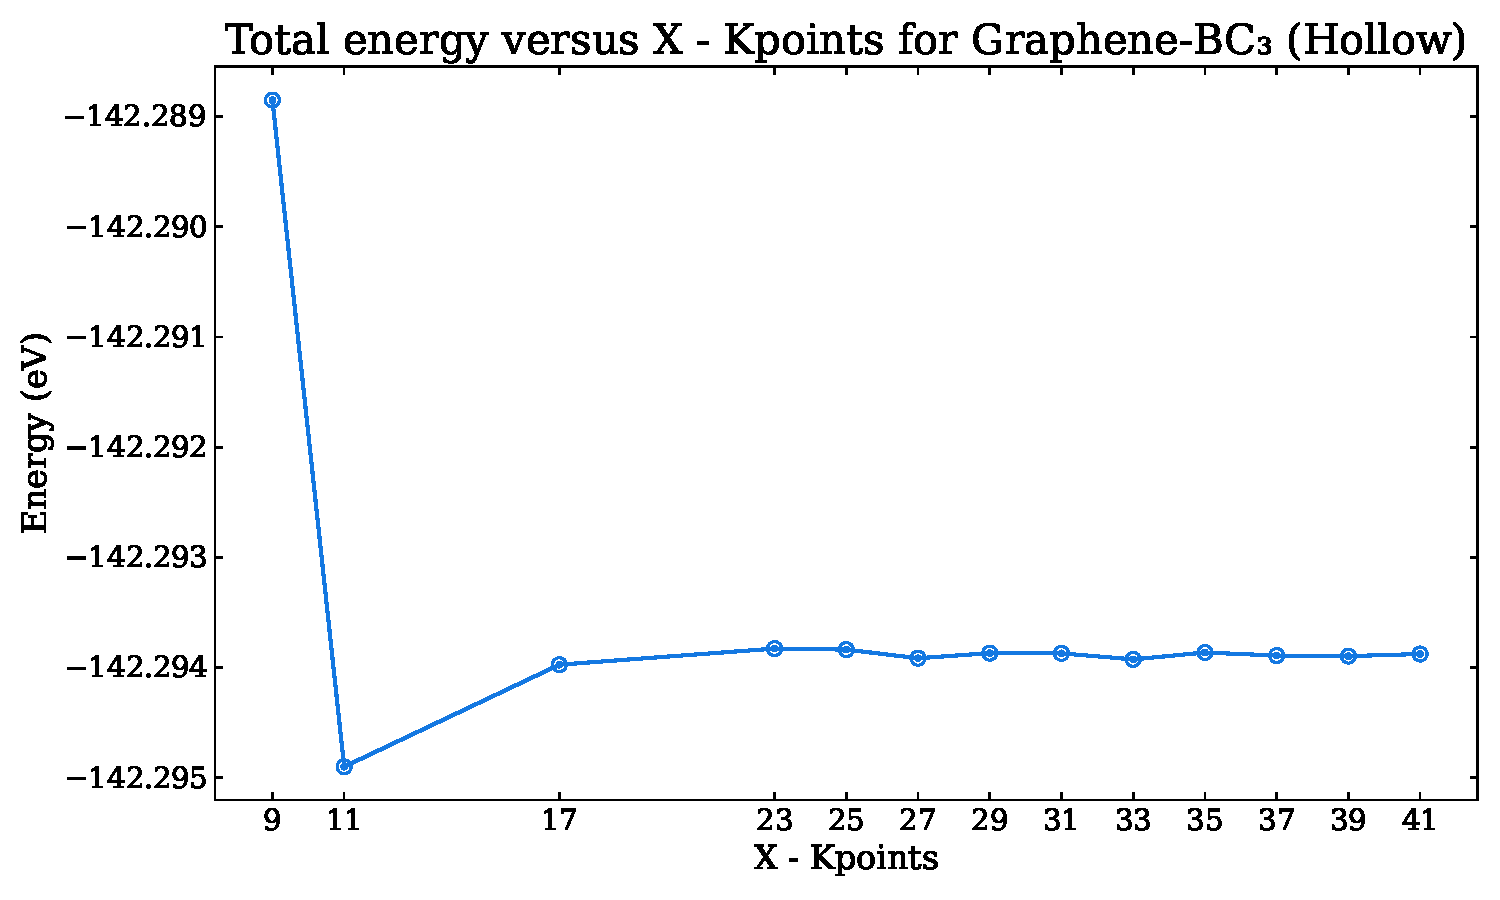
\includegraphics[width=0.6\textwidth]{figures_proj1/S1.1.pdf}
    \caption{Total energy versus the number of $\vec{k}$-points used to sample the Brillouin zone for the \ce{Graphene-BC3} bilayer system. Here, $\mathrm{X}$ denotes an $\mathrm{X}\times\mathrm{X}\times 1$ $\vec{k}$-point mesh.}
    \label{S1.1}
\end{figure}

\begin{figure}[!htbp]
    \centering
    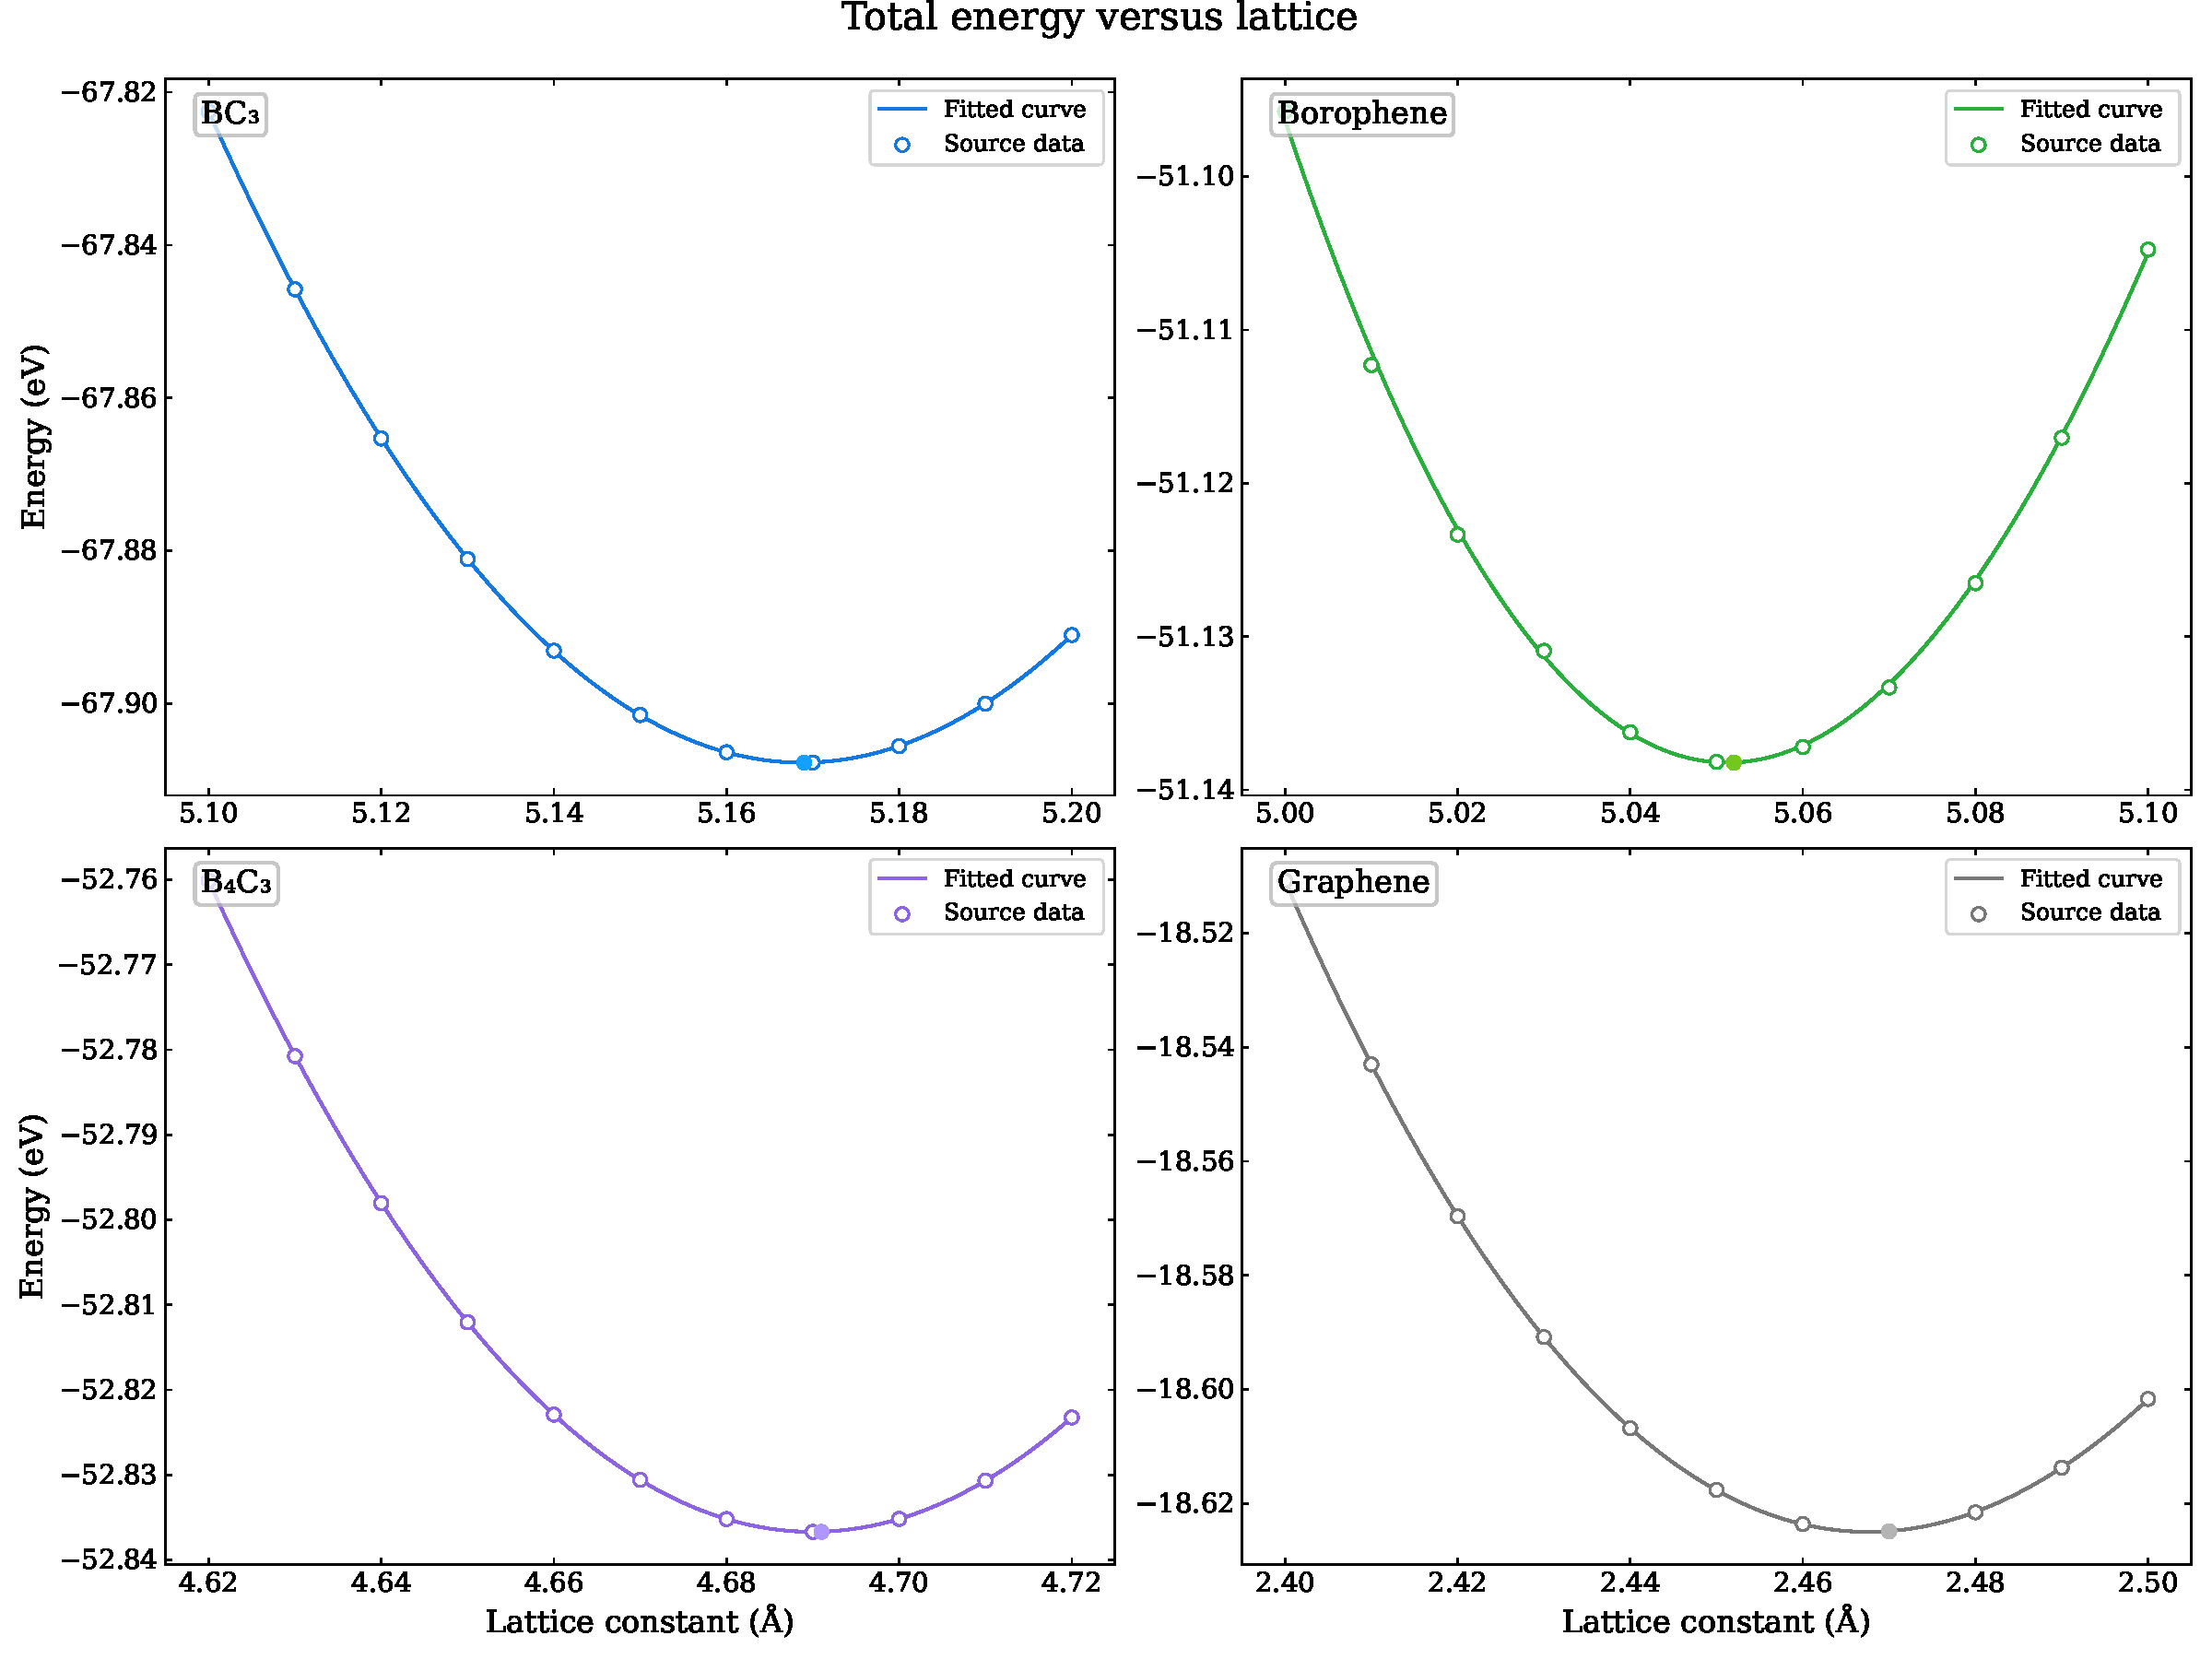
\includegraphics[width=0.80\textwidth]{figures_proj1/S1.2.pdf}
    \caption{Total energy versus lattice constant for the four monolayer systems: Graphene, borophene, \ce{BC3}, and \ce{B4C3}.
    The lattice constant yielding the lowest energy is shown by the full circle in each plot.}
    \label{S1.2}
\end{figure}

\begin{figure}[!htbp]
    \centering
    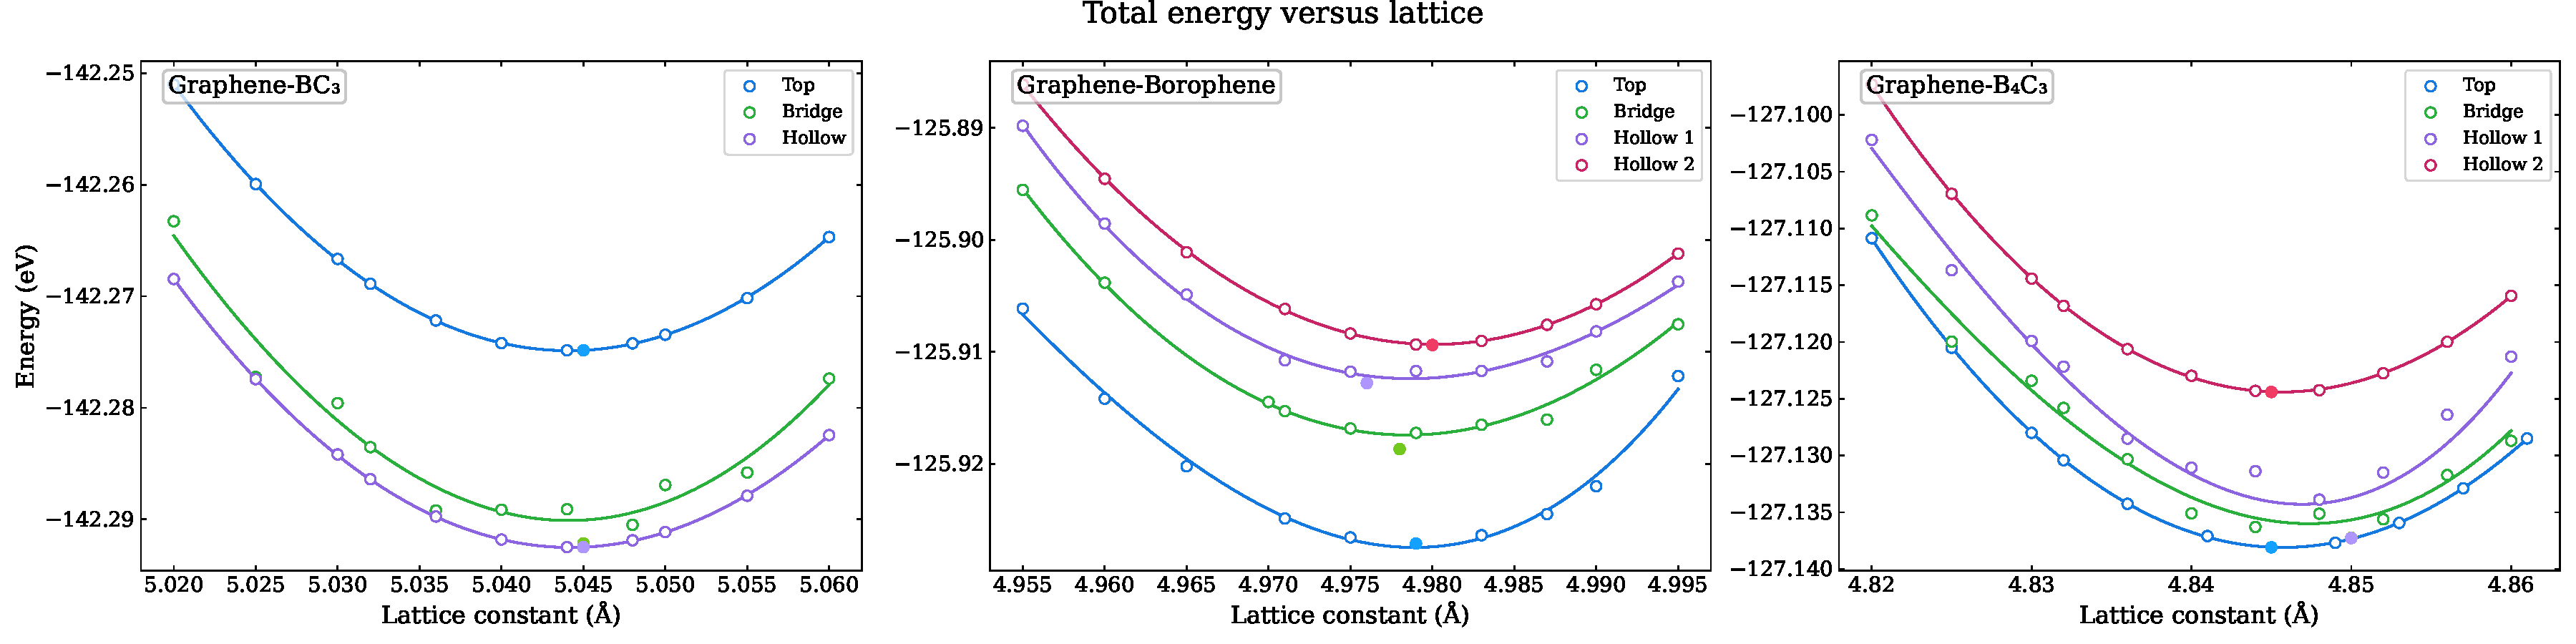
\includegraphics[width=1.00\textwidth]{figures_proj1/S1.3.pdf}
    \caption{Total energy versus lattice constant for the four monolayer systems: Graphene, borophene, \ce{BC3}, and \ce{B4C3}.
    Total energy versus lattice constant for each bilayer system for the various stacking positions considered.
    The lines are fitted curves with the full circle indicating the lowest energy structure.}
    \label{S1.3}
\end{figure}

\clearpage Figures~\ref{S1.4}--\ref{S1.6} show the total energy as a function of the lattice constant and interlayer distance for the various lateral positions considered.
In each figure, the equilibrium geometry is indicated by the ``Extrema of fitted data'' result.

\begin{figure}[!htbp]
\centering
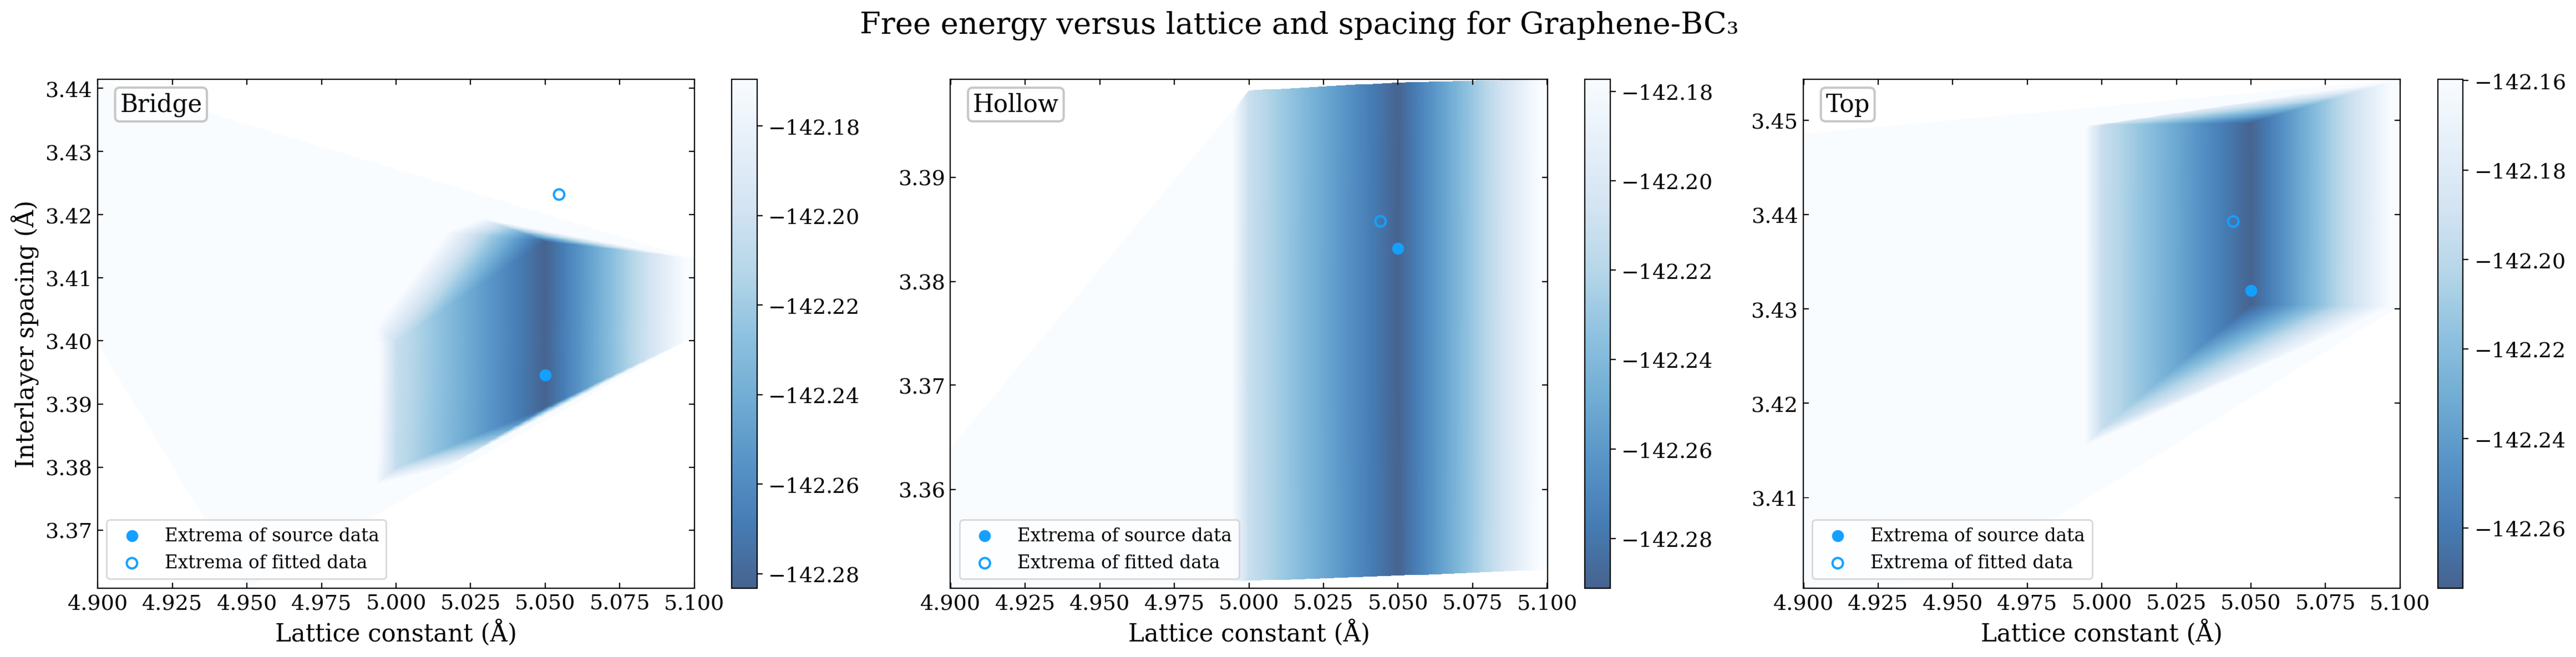
\includegraphics[width=1.00\textwidth]{figures_proj1/S1.4.pdf}
\caption{Total-energy landscape of the \ce{Graphene-BC3} bilayer.}
\label{S1.4}
\end{figure}

\begin{figure}[!htbp]
\centering
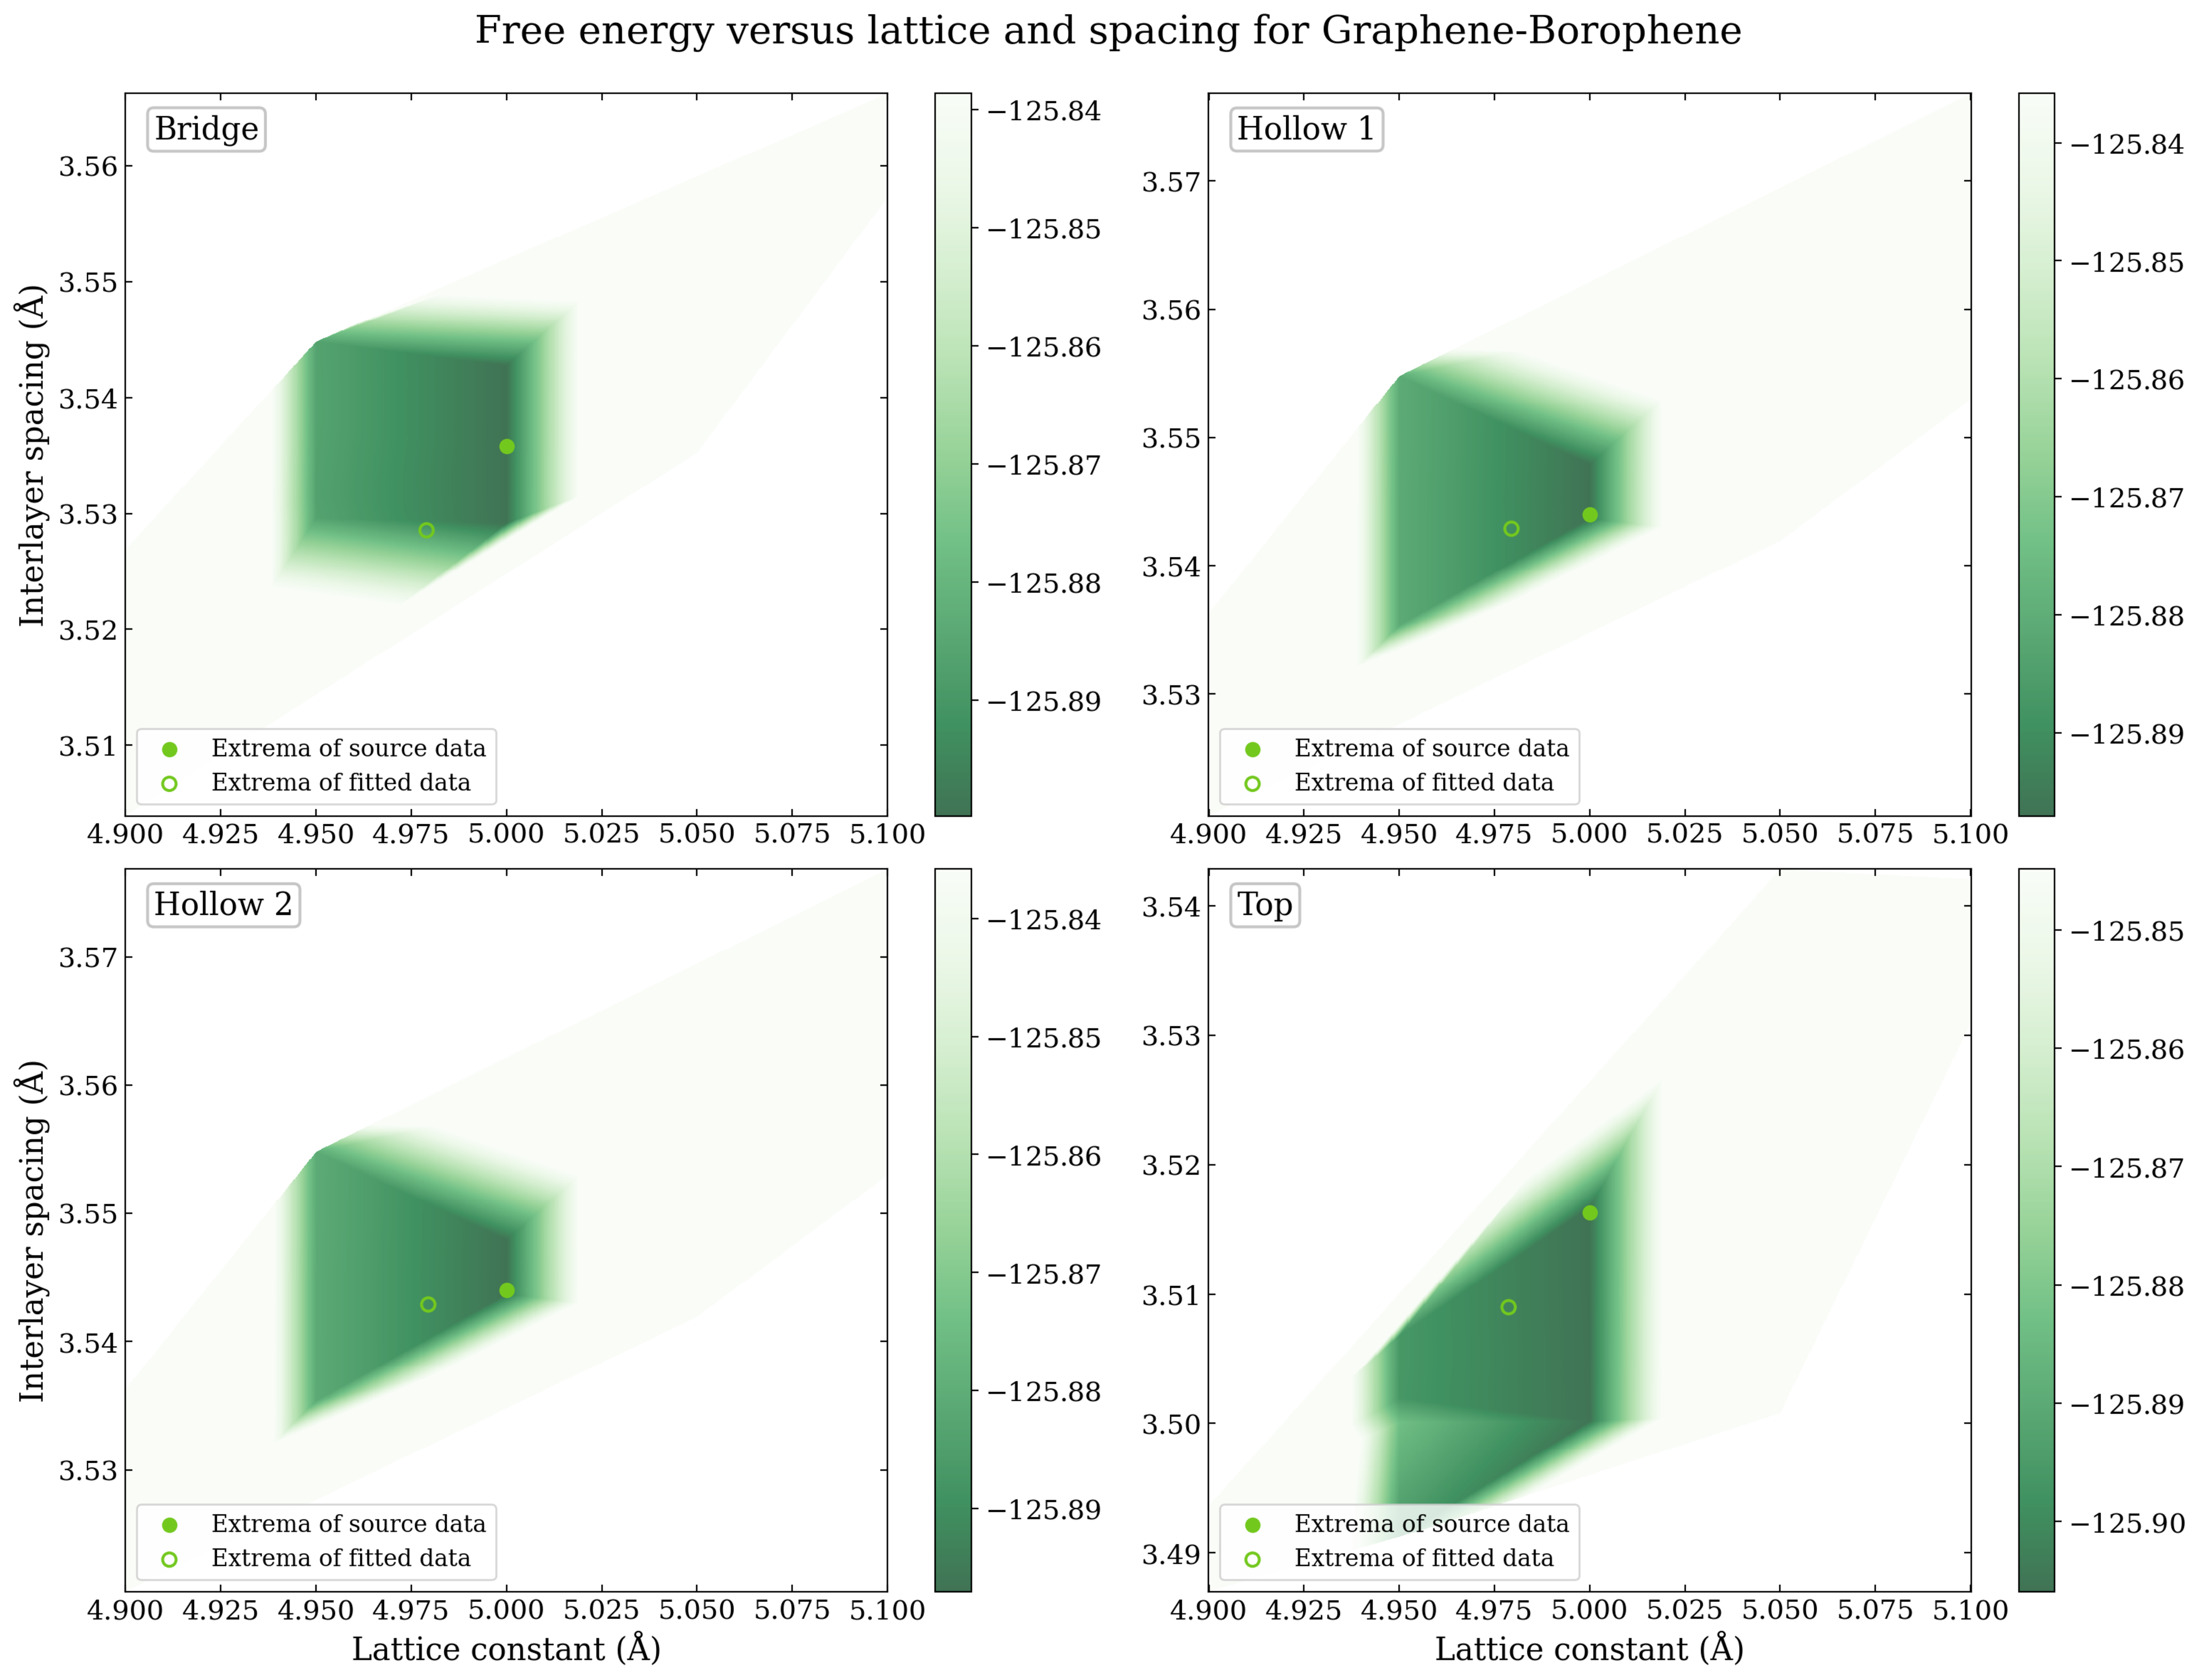
\includegraphics[width=0.80\textwidth]{figures_proj1/S1.5.pdf}
\caption{Total-energy landscape of the \ce{Graphene-Borophene} bilayer.}
\label{S1.5}
\end{figure}

\begin{figure}[!htbp]
\centering
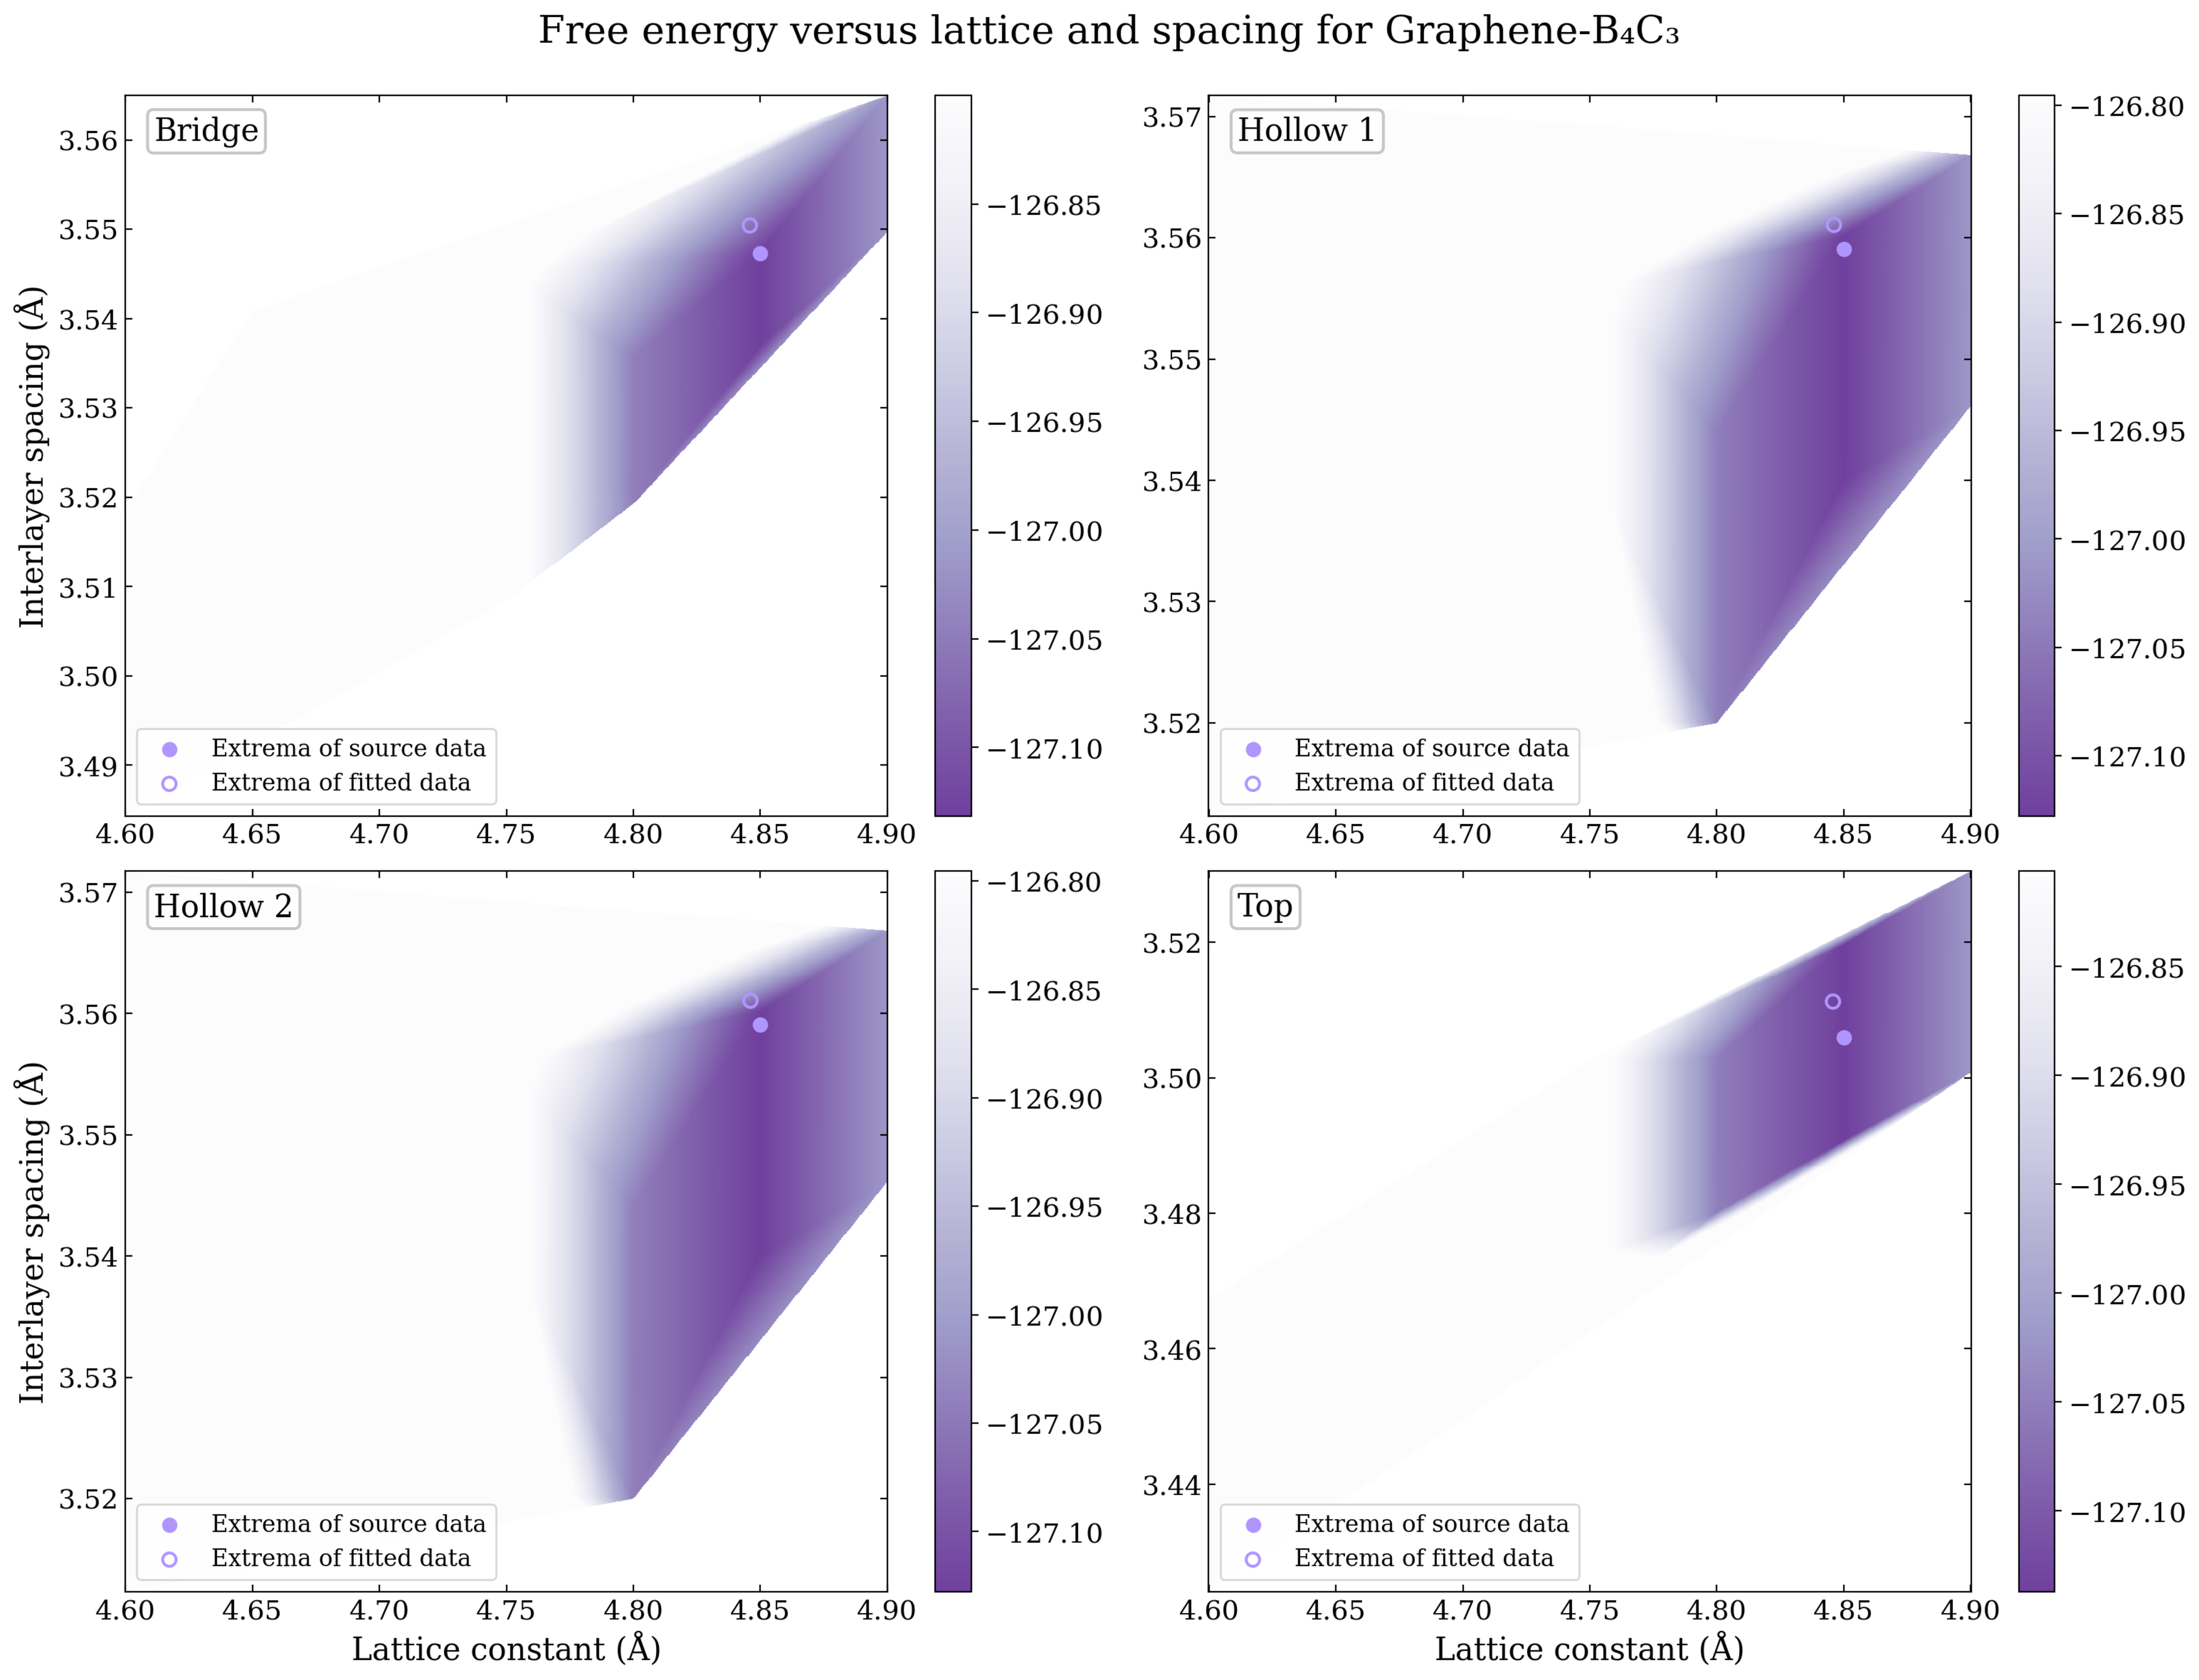
\includegraphics[width=0.80\textwidth]{figures_proj1/S1.6.pdf}
\caption{Total-energy landscape of the \ce{Graphene-B4C3} bilayer.}
\label{S1.6}
\end{figure}

\begin{table}[!htbp]
\centering
\begin{adjustbox}{max width=1.0\linewidth}
\begin{tabular}{cm{60px}m{110px}m{120px}m{90px}m{100px}}
\hline
\rowcolor{gray!25}
system
& site
& lattice constant (Å)
& inter-planar spacing (Å)
& total energy (eV)
& relative energy (eV) \\ \hline

\multirow{3}{*}{\ce{Graphene-BC3}}
& Top
& 5.044
& 3.432
& -142.275
& 0.018 \\

& \cellcolor{gray!15} Bridge
& \cellcolor{gray!15} 5.044
& \cellcolor{gray!15} 3.384
& \cellcolor{gray!15} -142.290
& \cellcolor{gray!15} 0.002 \\

& \textbf{Hollow}
& \textbf{5.044}
& \textbf{3.375}
& \textbf{-142.293}
& \textbf{0.000} \\ \hline

\cellcolor{gray!15}
& \textbf{Top}
& \textbf{4.979}
& \textbf{3.496}
& \textbf{-125.927}
& \textbf{0.000} \\

\rowcolor{gray!15}
\cellcolor{gray!15}
& Bridge
& 4.979
& 3.505
& -125.921
& 0.006 \\

\cellcolor{gray!15}
& Hollow 1
& 4.979
& 3.551
& -125.914
& 0.013 \\

\rowcolor{gray!15}
\cellcolor{gray!15}
\multirow{-4}{*}{\ce{Graphene-Borophene}}
& Hollow 2
& 4.979
& 3.548
& -125.909
& 0.018 \\ \hline

\cellcolor{white}
& \textbf{Top}
& \textbf{4.846}
& \textbf{3.514}
& \textbf{-127.138}
& \textbf{0.000} \\

\rowcolor{gray!15}
\cellcolor{white}
& Bridge
& 4.846
& 3.536
& -127.135
& 0.003 \\

\cellcolor{white}
& Hollow 1
& 4.846
& 3.545
& -127.133
& 0.005 \\

\rowcolor{gray!15}
\cellcolor{white}
\multirow{-4}{*}{\ce{Graphene-B4C3}}
& Hollow 2
& 4.846
& 3.562
& -127.124
& 0.014 \\ \hline

\end{tabular}
\end{adjustbox}
\caption{For each bilayer system and each lateral position considered, the optimized lattice constant, interlayer spacing, total energy, and relative energy are given.
The relative energy is given with respect to the most favourable structure, which corresponds to the lowest total energy for each bilayer system.}
\label{tab:S1.1}
\end{table}

\clearpage In addition, figures~\ref{S1.9}--\ref{S1.11} show the projected densities of states of the three heterostructure systems calculated using the HSE06 functional.

\begin{figure}[!htbp]
\centering
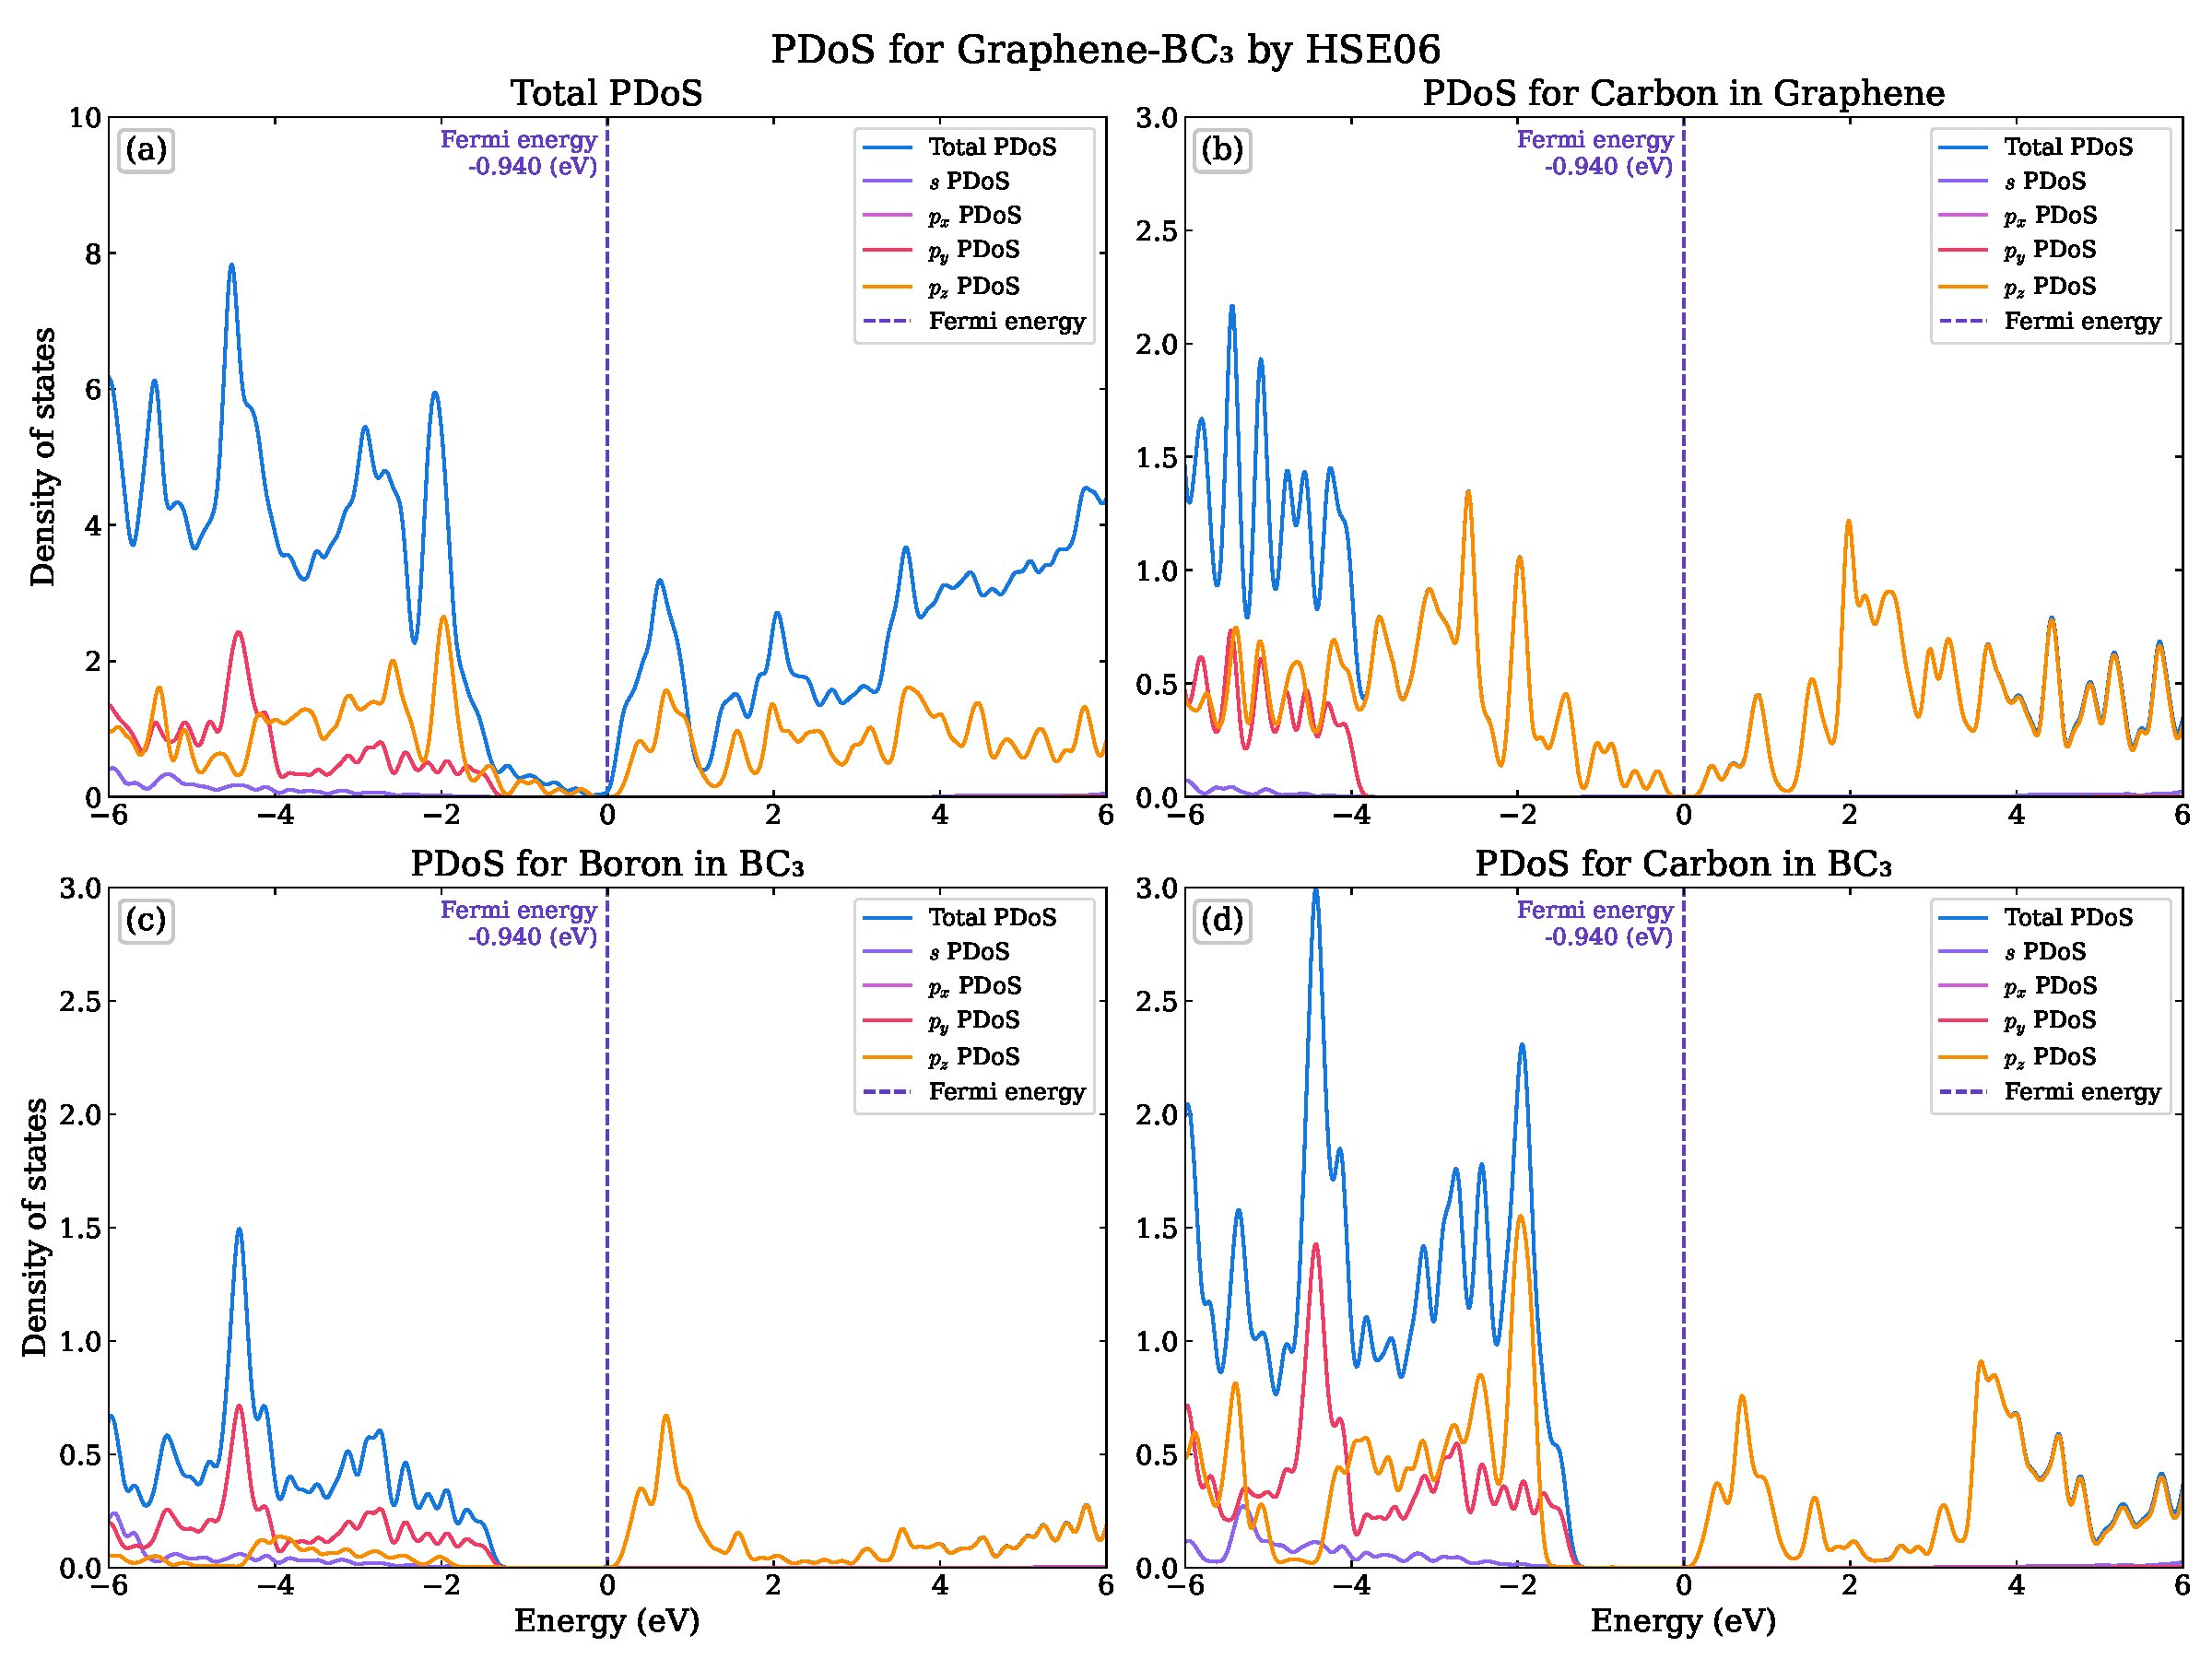
\includegraphics[width=0.80\textwidth]{figures_proj1/S1.9.pdf}
\caption{Projected density of states of \ce{Graphene-BC3} by HSE06.}
\label{S1.9}
\end{figure}

\begin{figure}[!htbp]
\centering
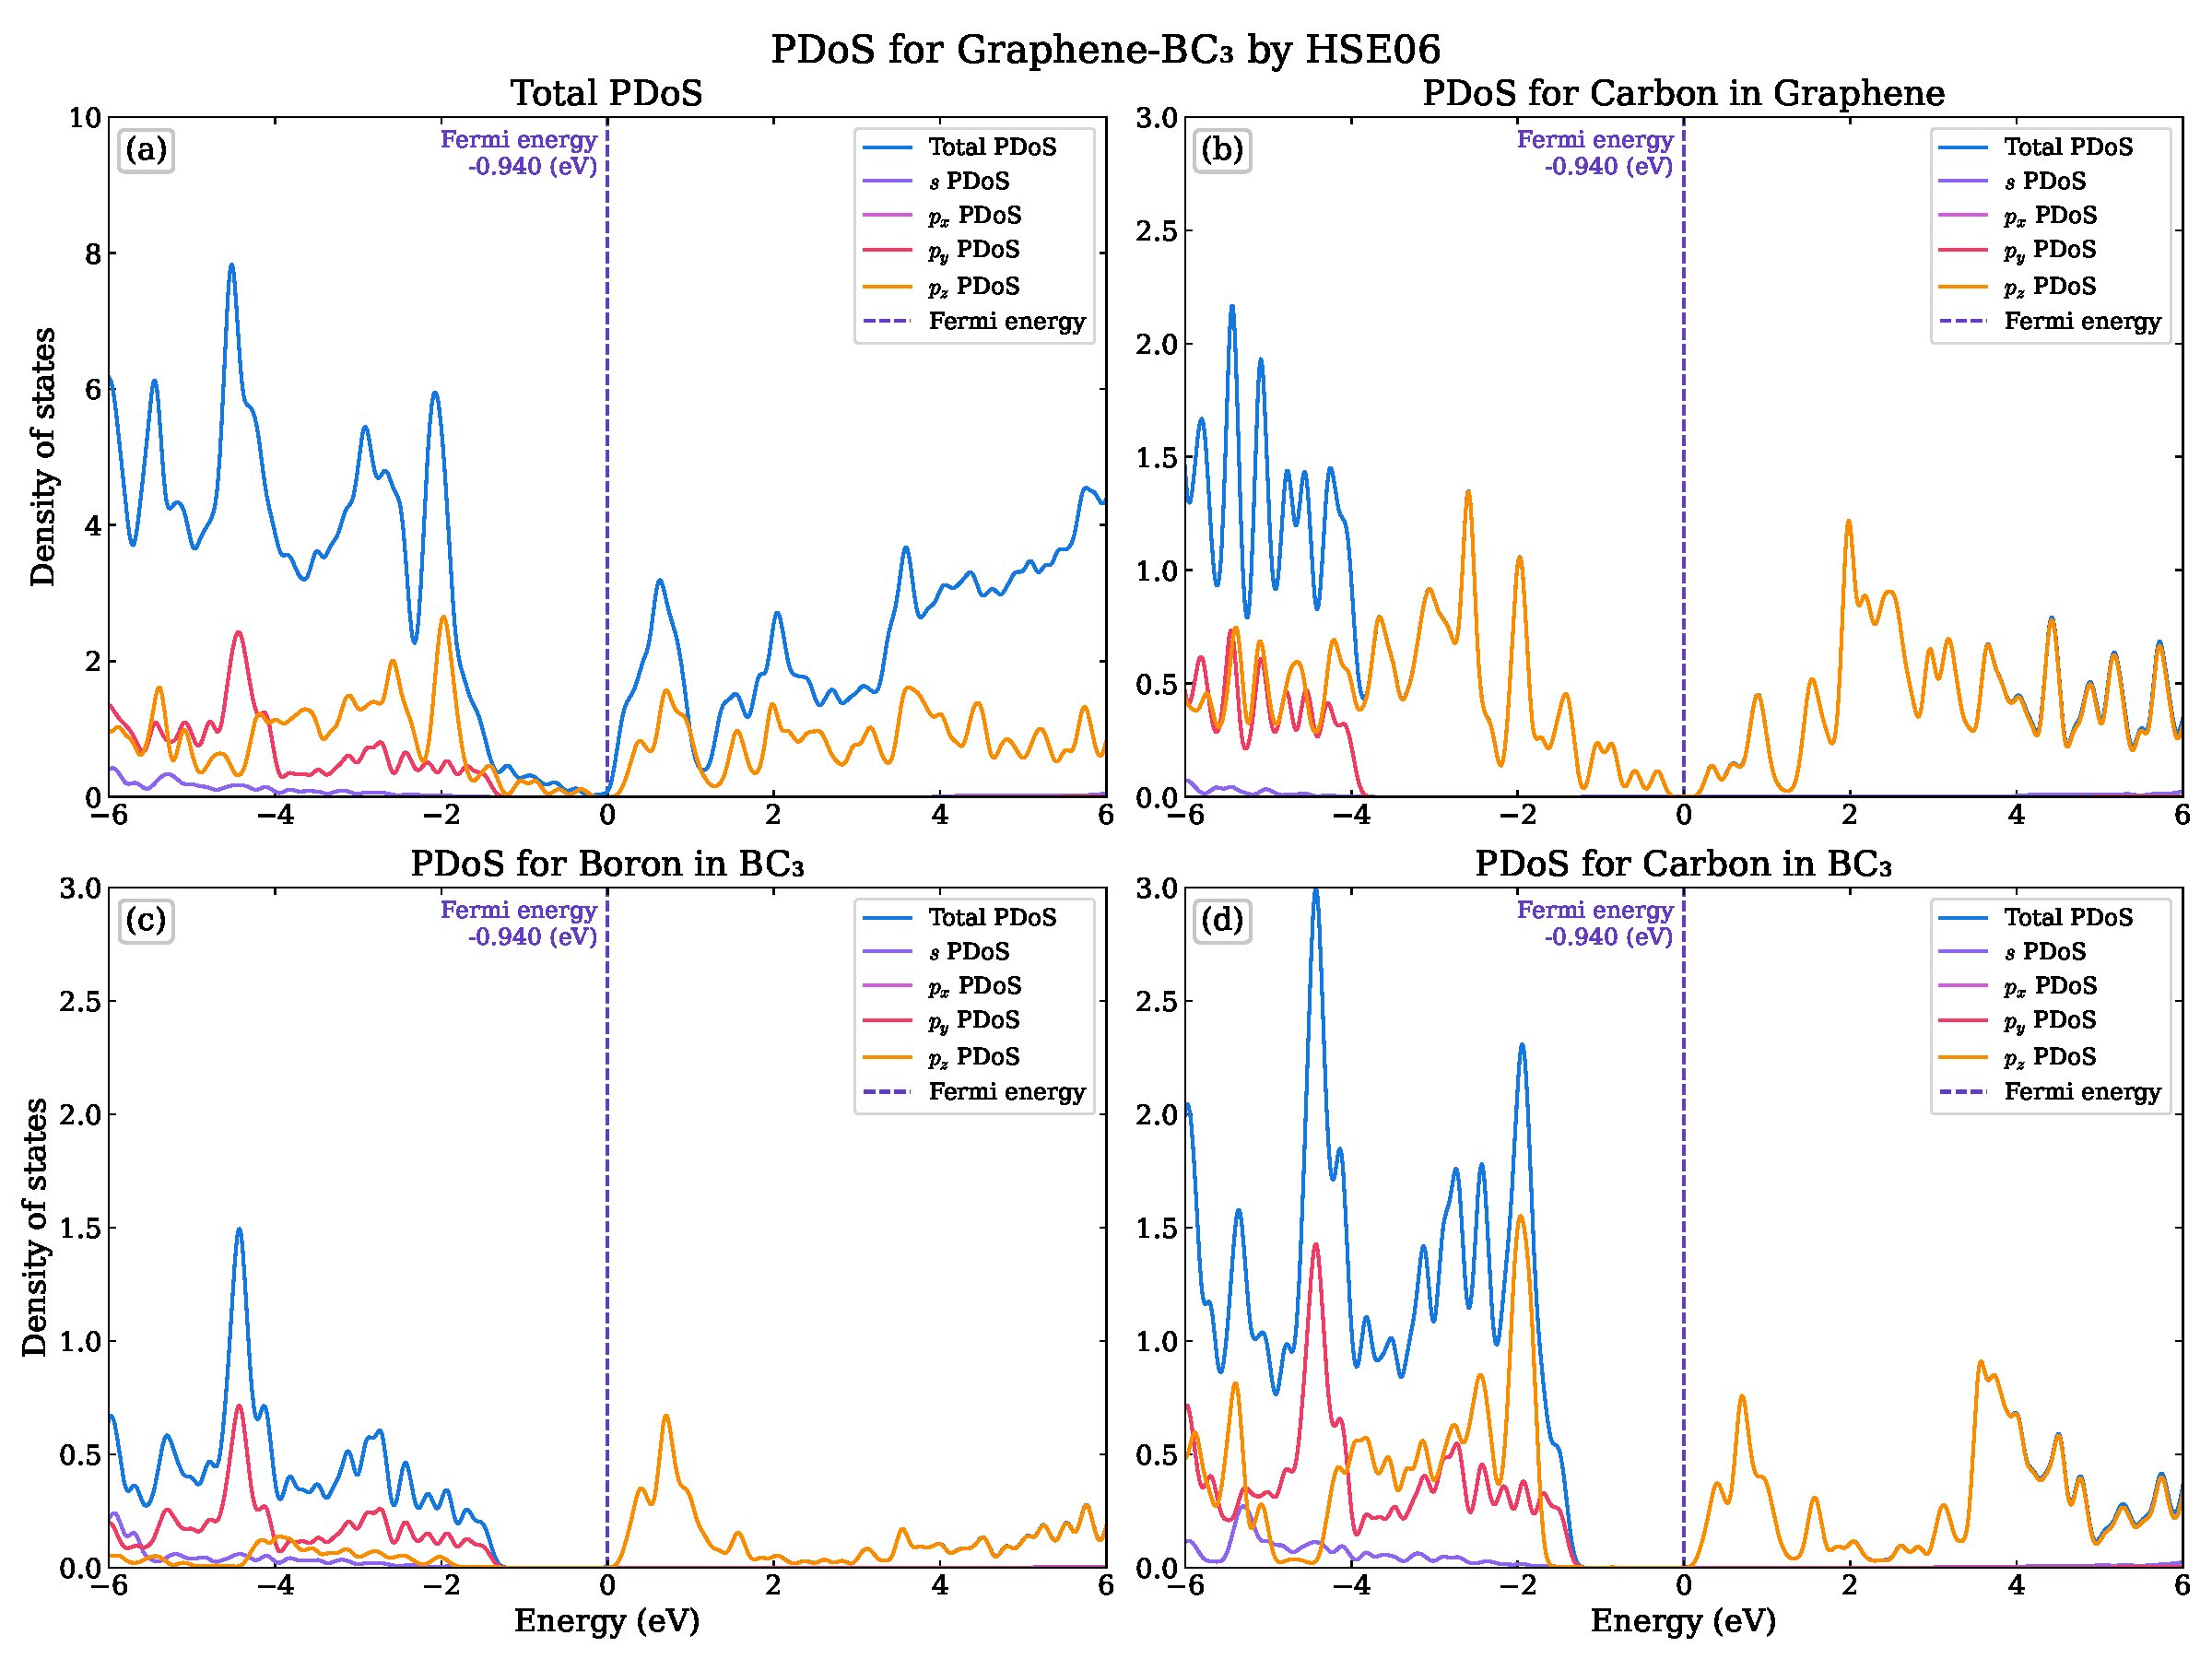
\includegraphics[width=1.0\textwidth]{figures_proj1/S1.10.pdf}
\caption{Projected density of states of \ce{Graphene-Borophene} by HSE06.}
\label{S1.10}
\end{figure}

\begin{figure}[!htbp]
\centering
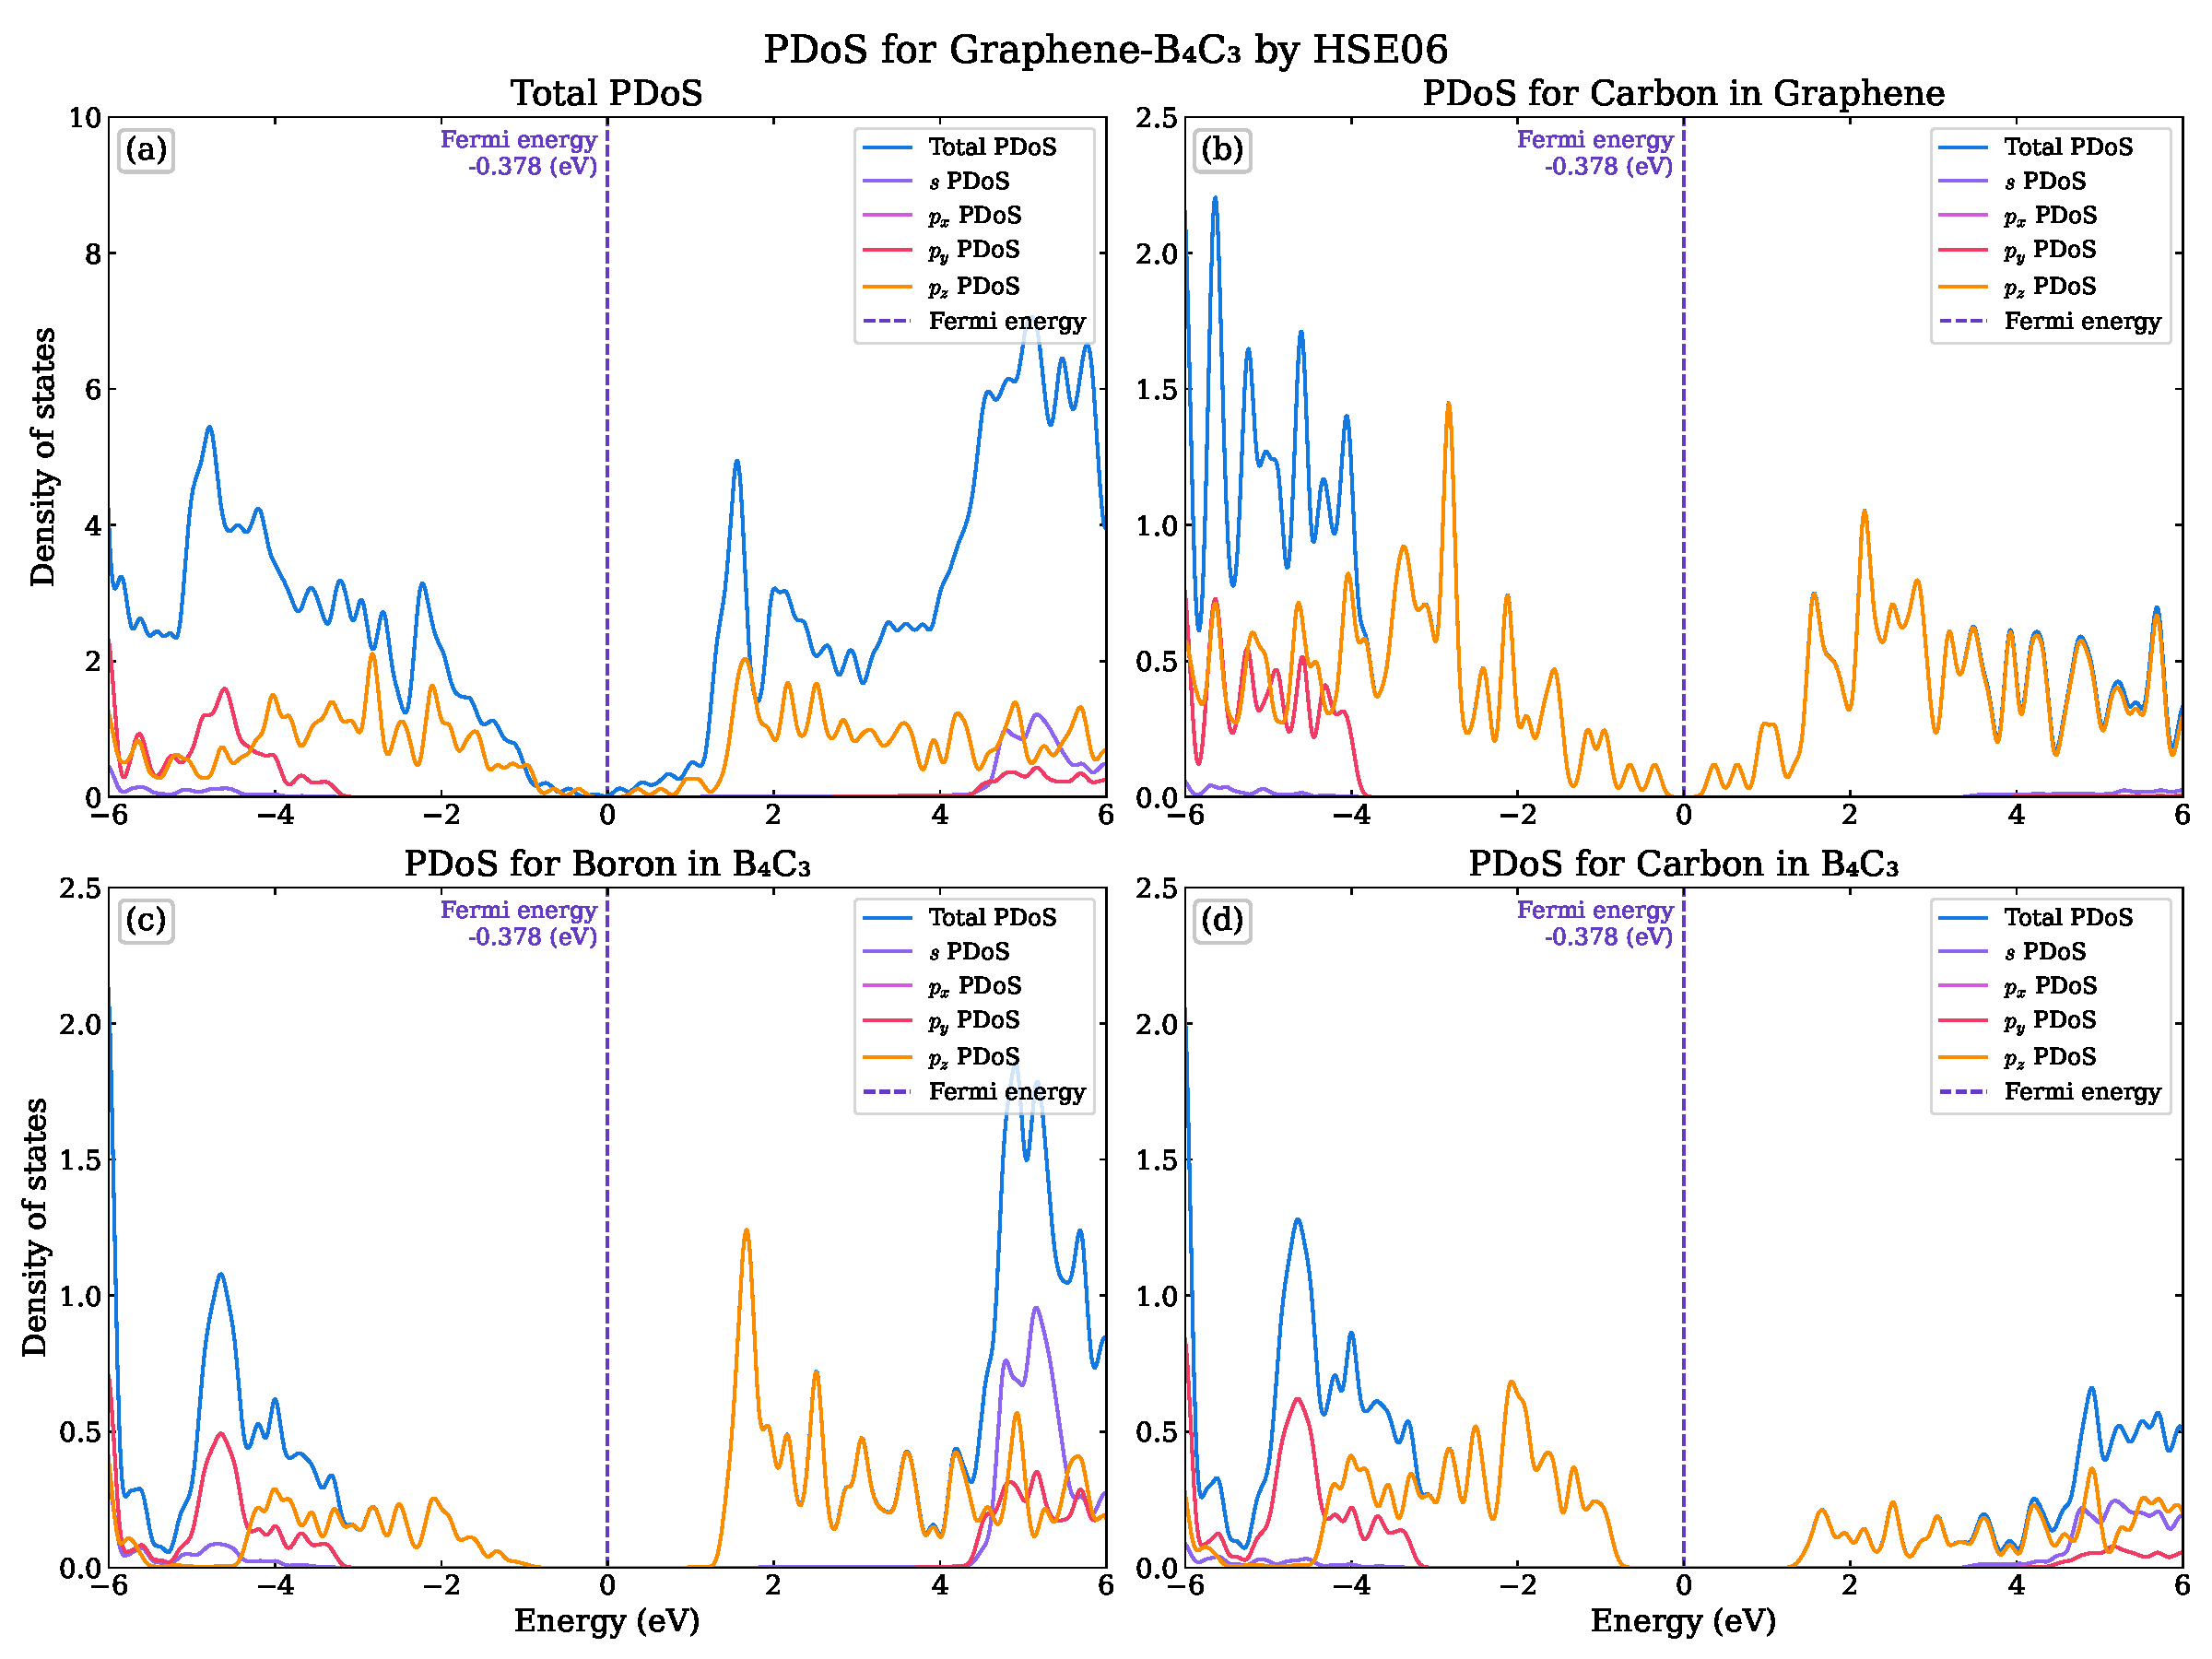
\includegraphics[width=0.80\textwidth]{figures_proj1/S1.11.pdf}
\caption{Projected density of states of \ce{Graphene-B4C3} by HSE06.}
\label{S1.11}
\end{figure}

\begin{figure}[!htbp]
\centering
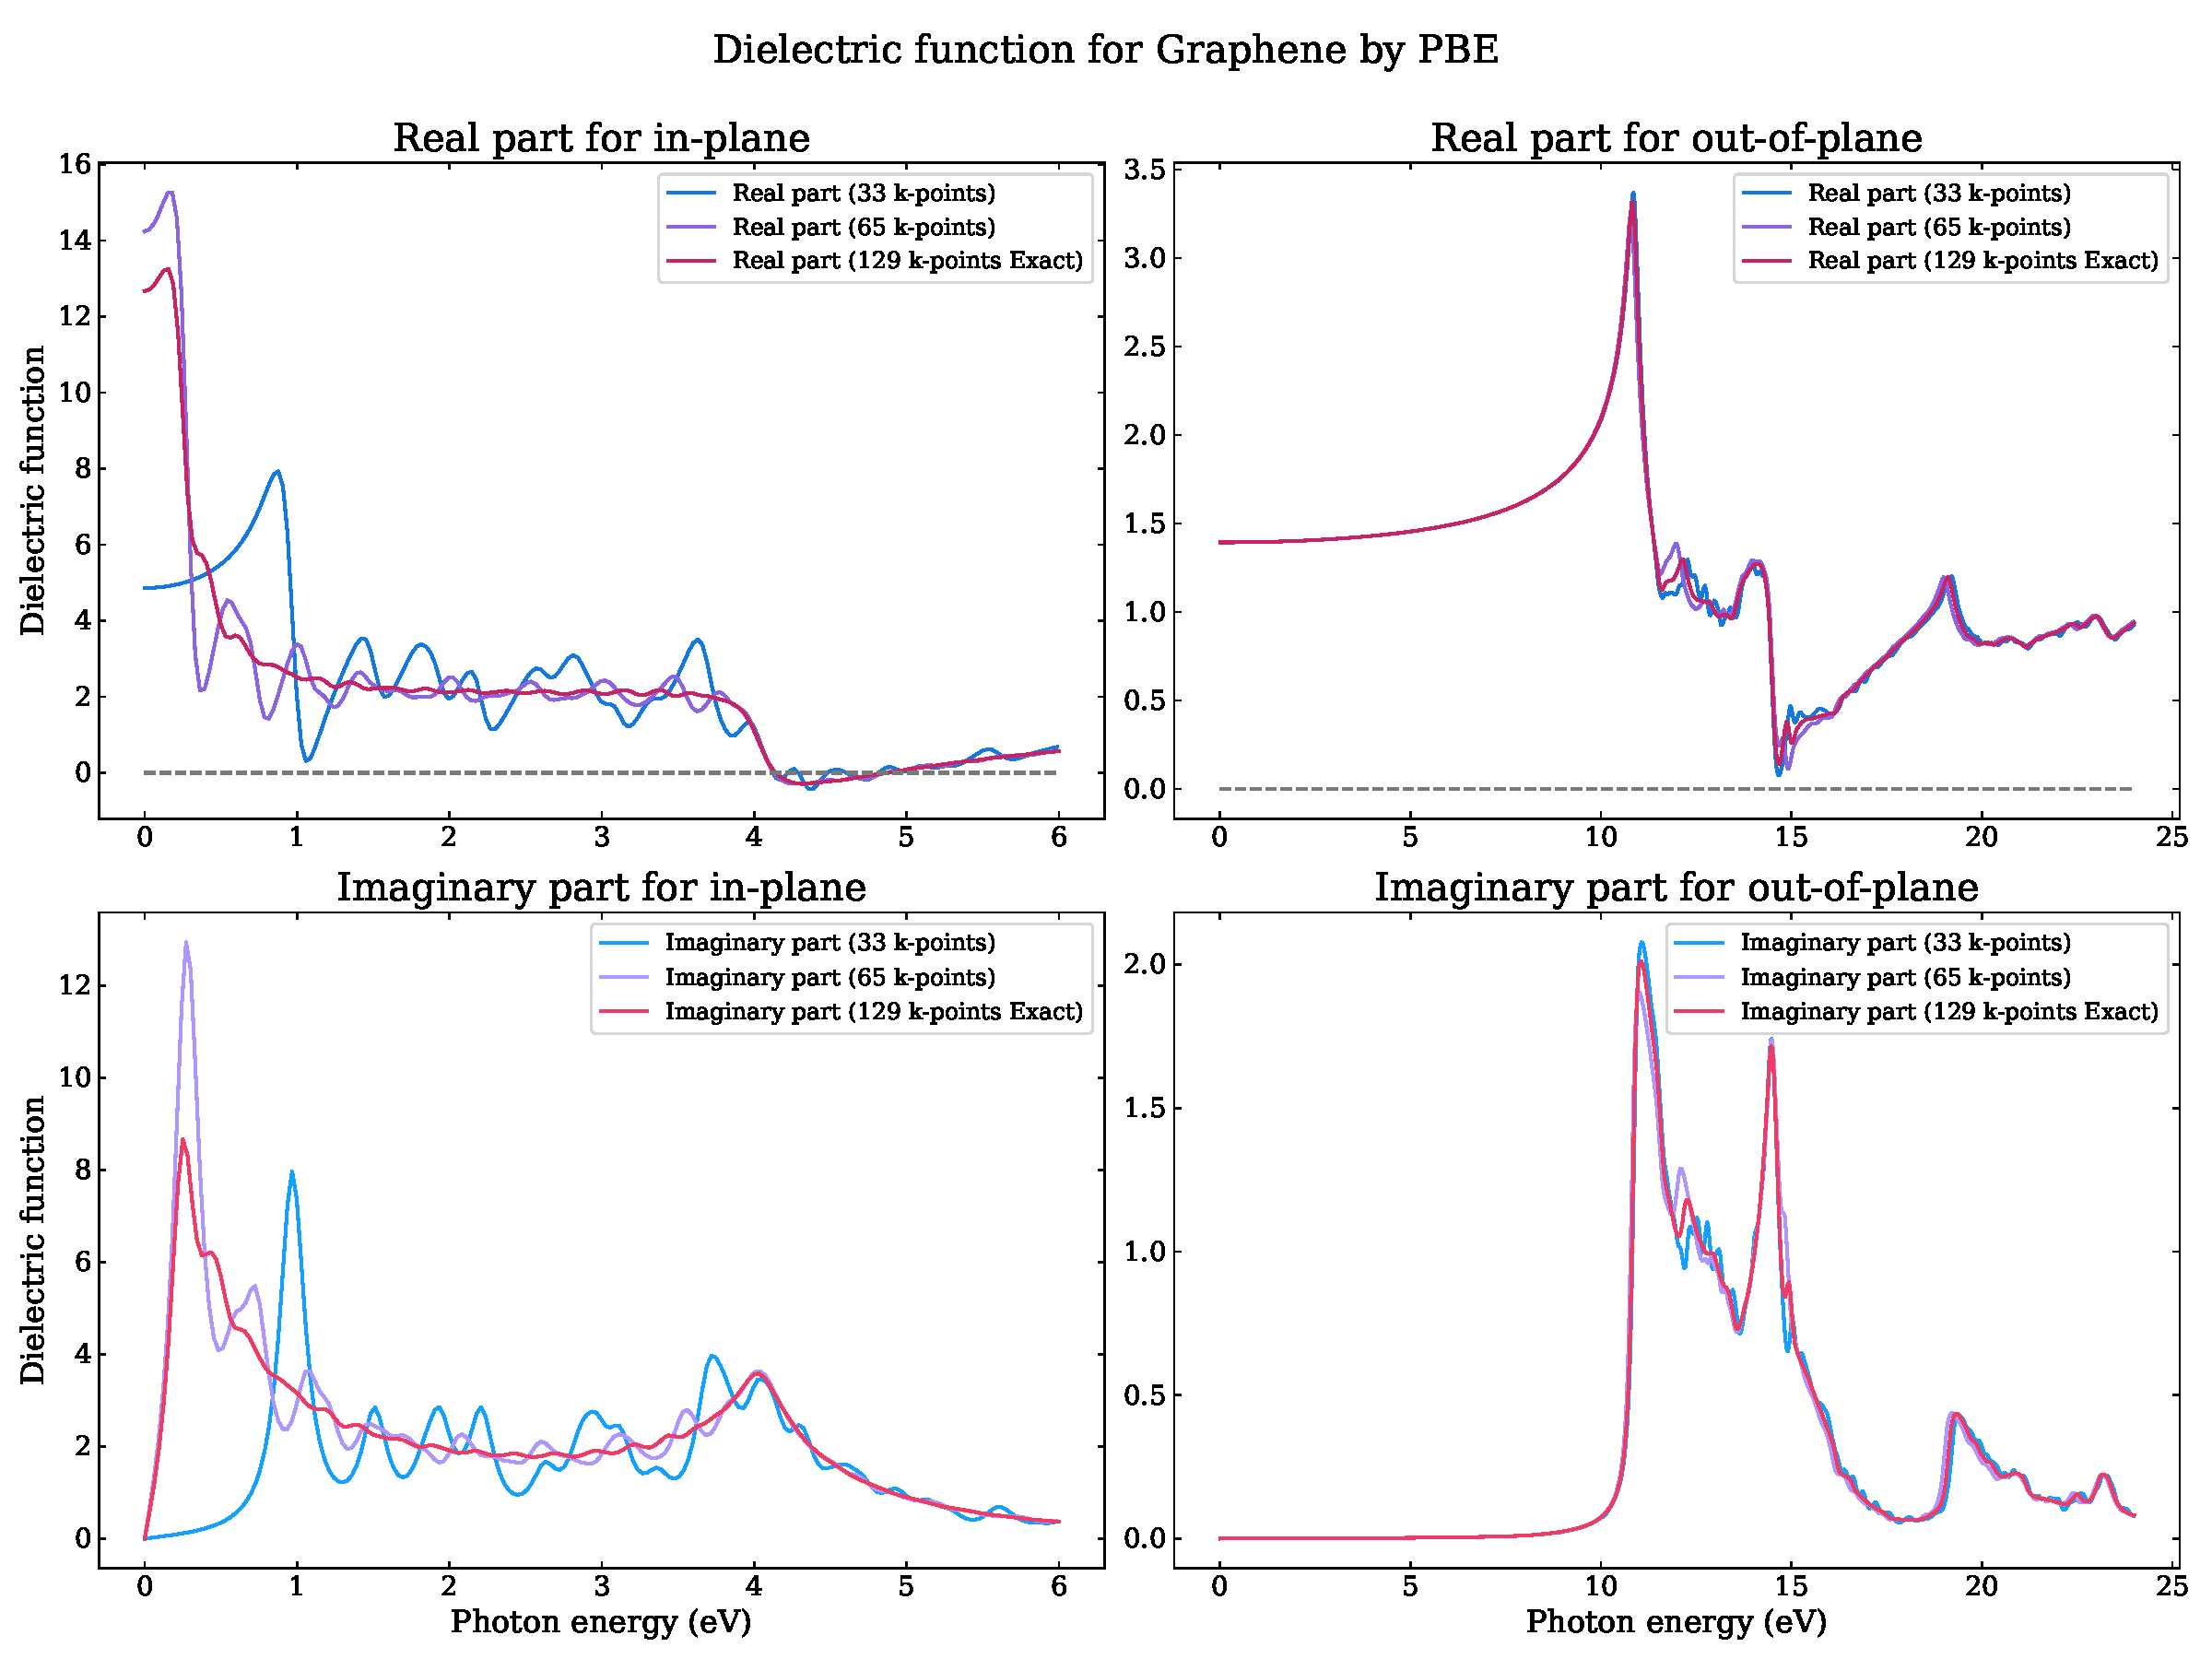
\includegraphics[width=0.80\textwidth]{figures_proj1/S1.12.pdf}
\caption{Dielectric function of graphene calculated using the PBE functional for different $\vec{k}$-point meshes,
where, for example,
$33$ denotes a $33 \times 33 \times 1$ $\vec{k}$-point mesh.}
\label{S1.12}
\end{figure}

\begin{figure}[!htbp]
    \centering
    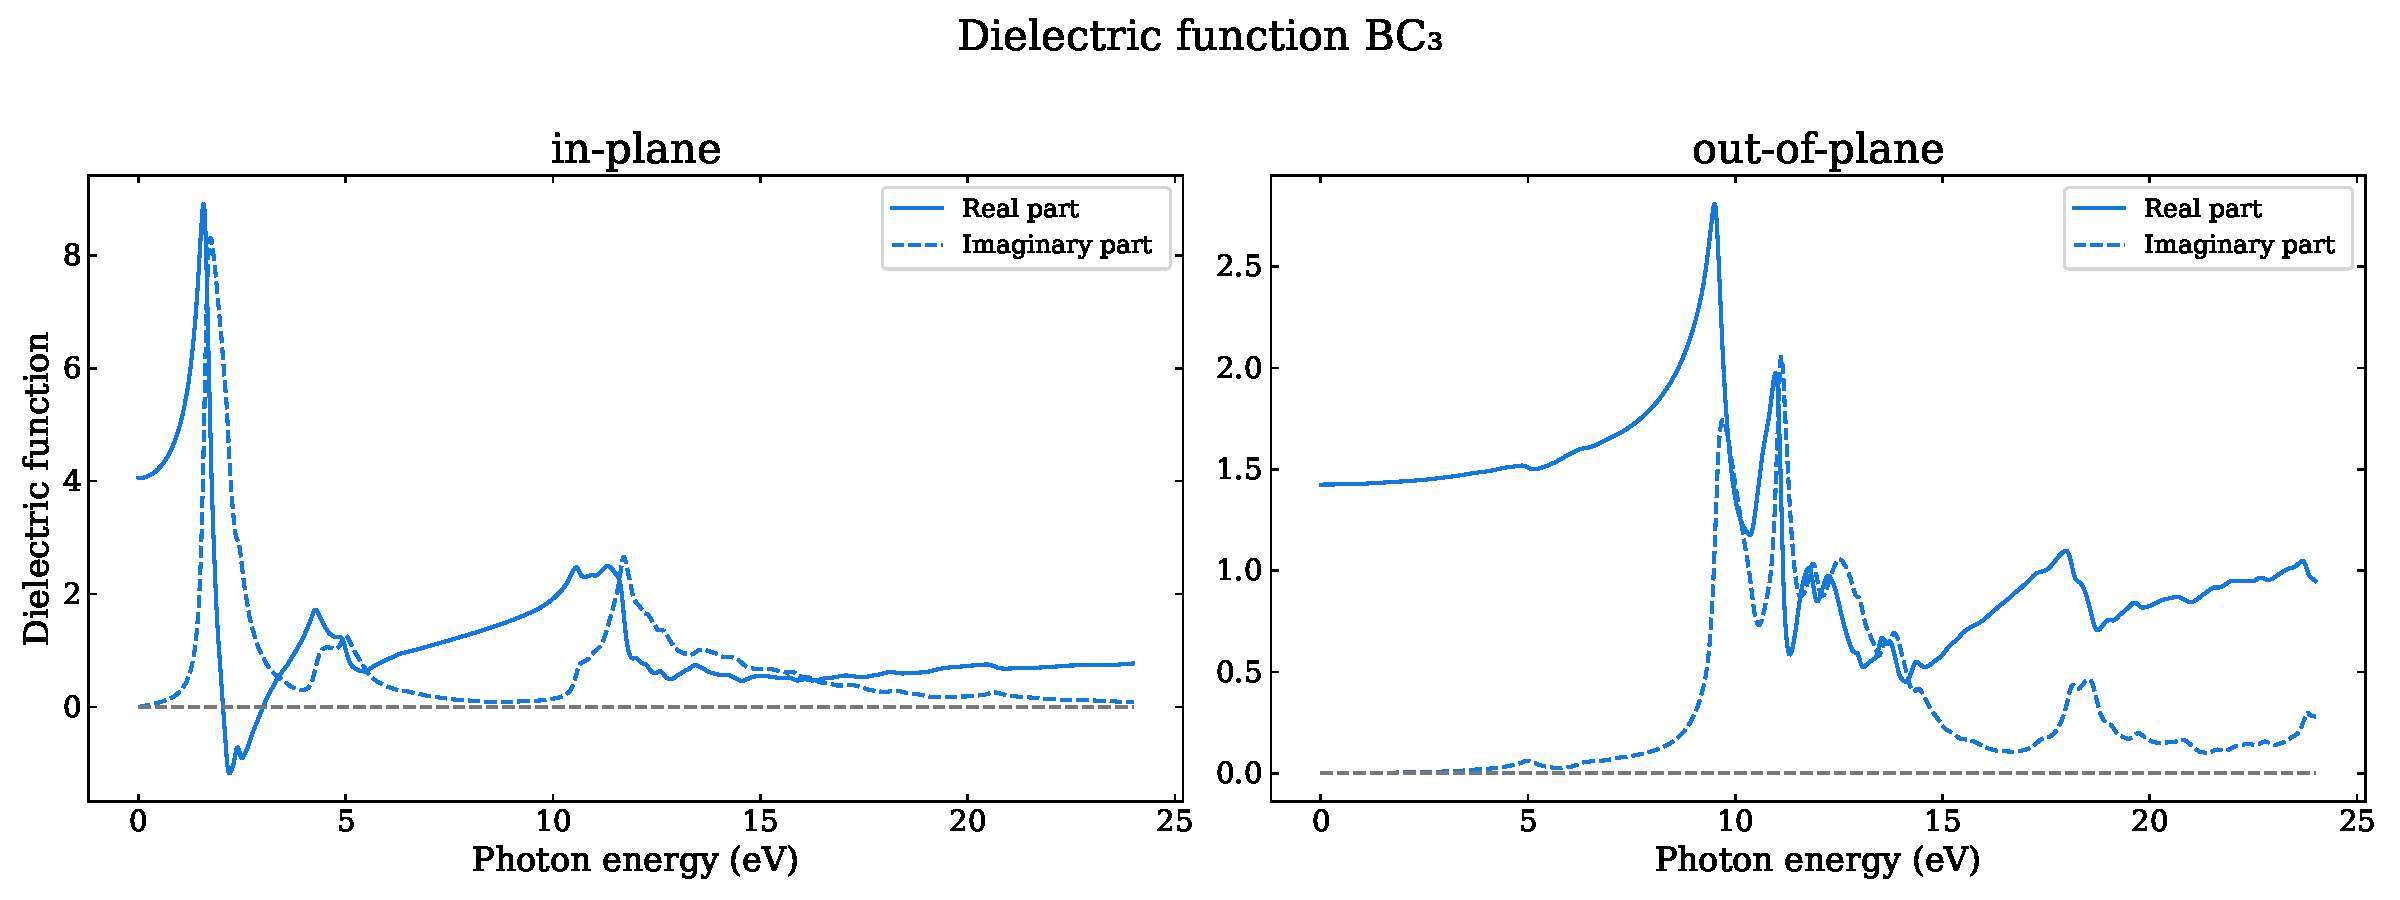
\includegraphics[width=0.80\linewidth]{figures_proj1/S1.13a.pdf}
    \par\nointerlineskip
    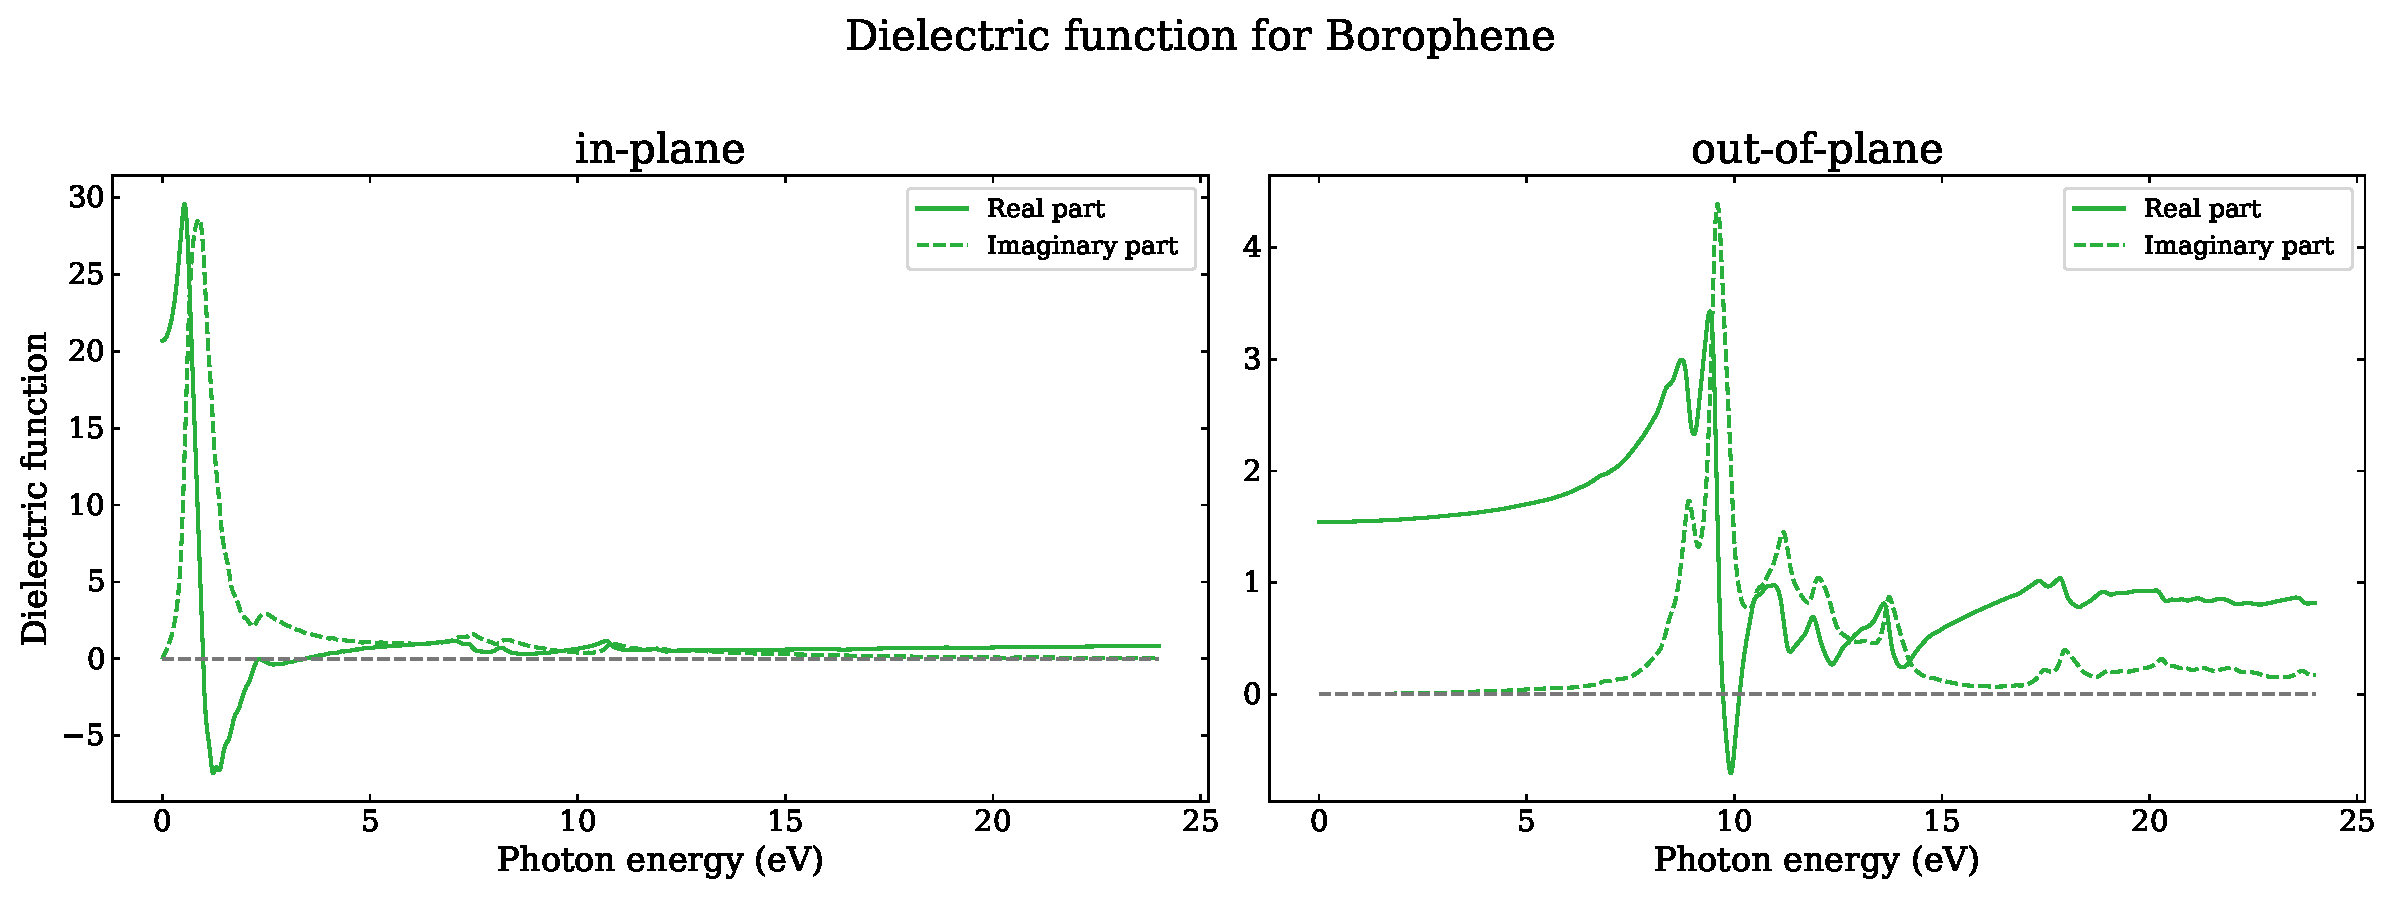
\includegraphics[width=0.80\linewidth]{figures_proj1/S1.13b.pdf}
    \par\nointerlineskip
    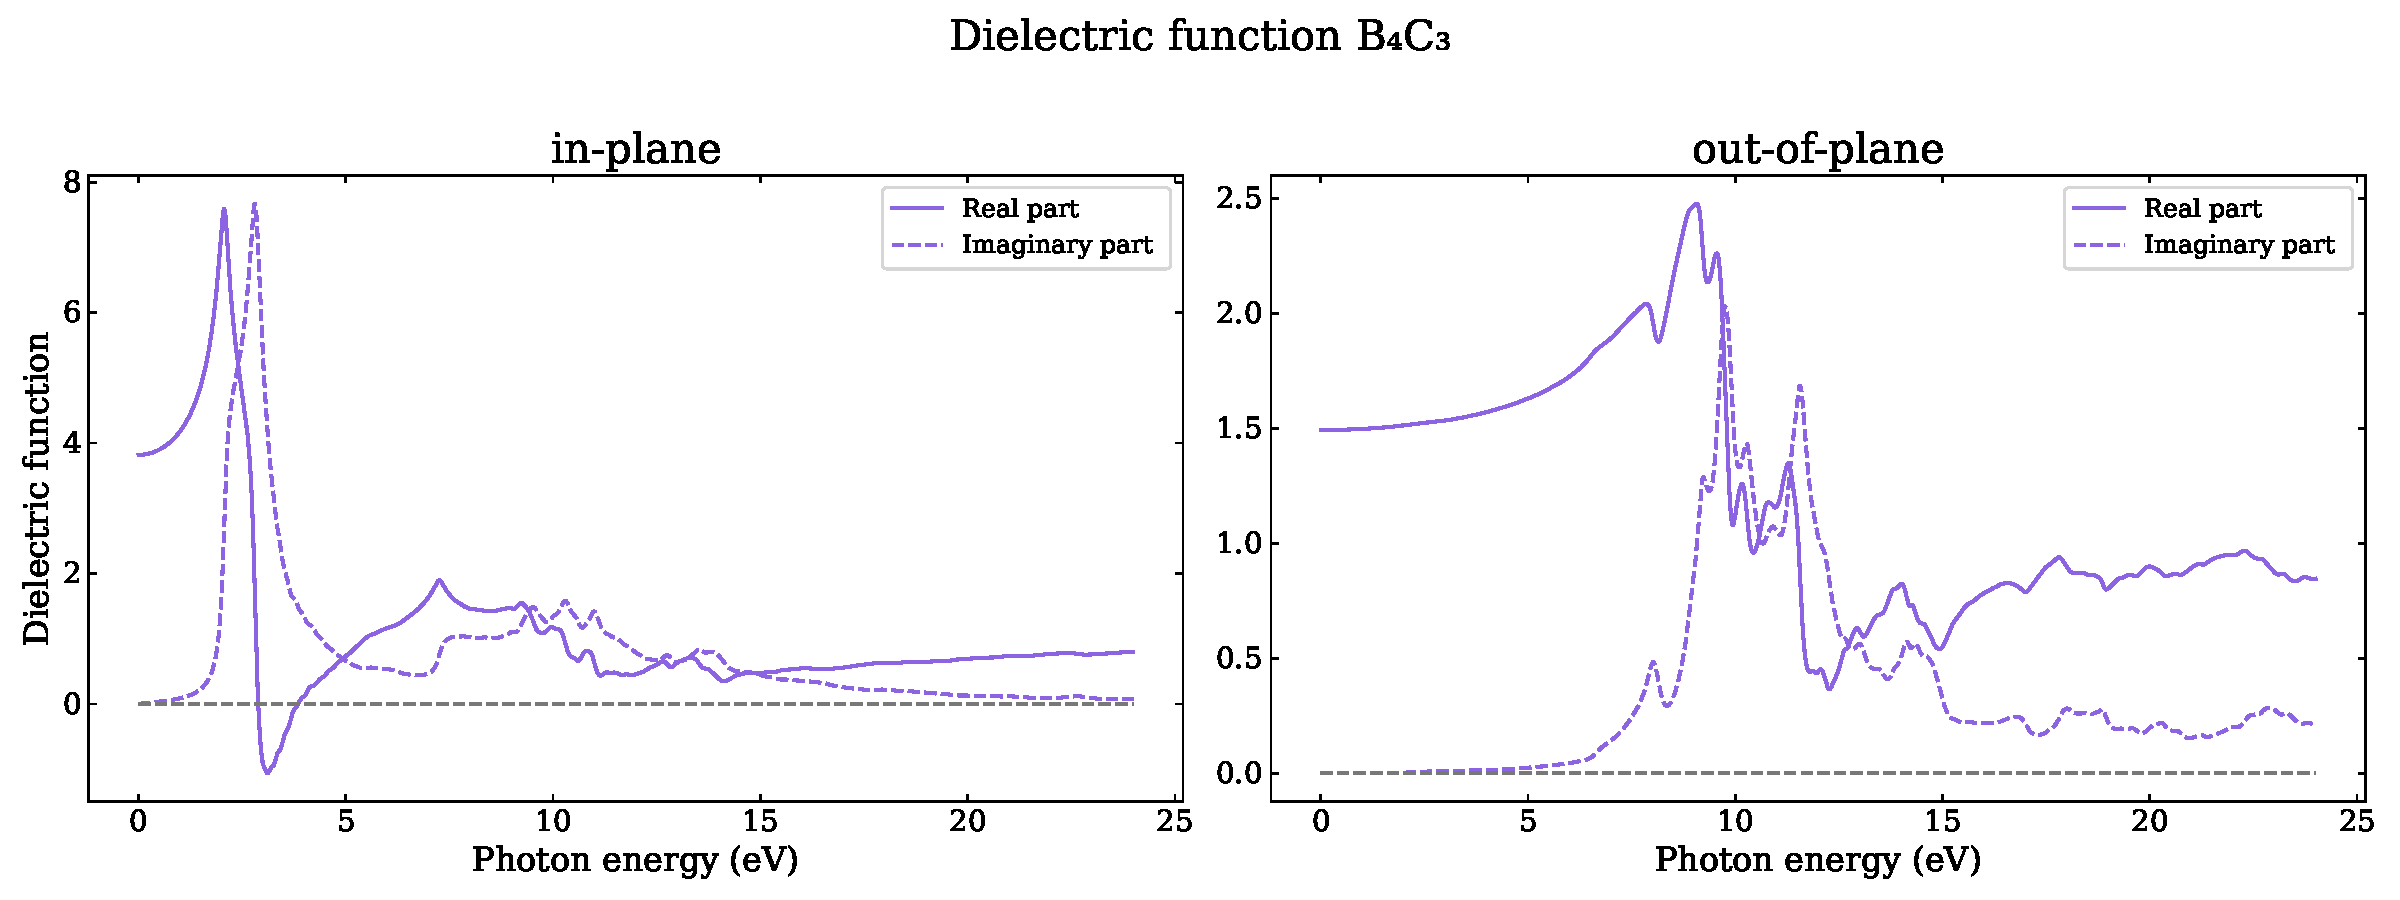
\includegraphics[width=0.80\linewidth]{figures_proj1/S1.13c.pdf}
    \par\nointerlineskip
    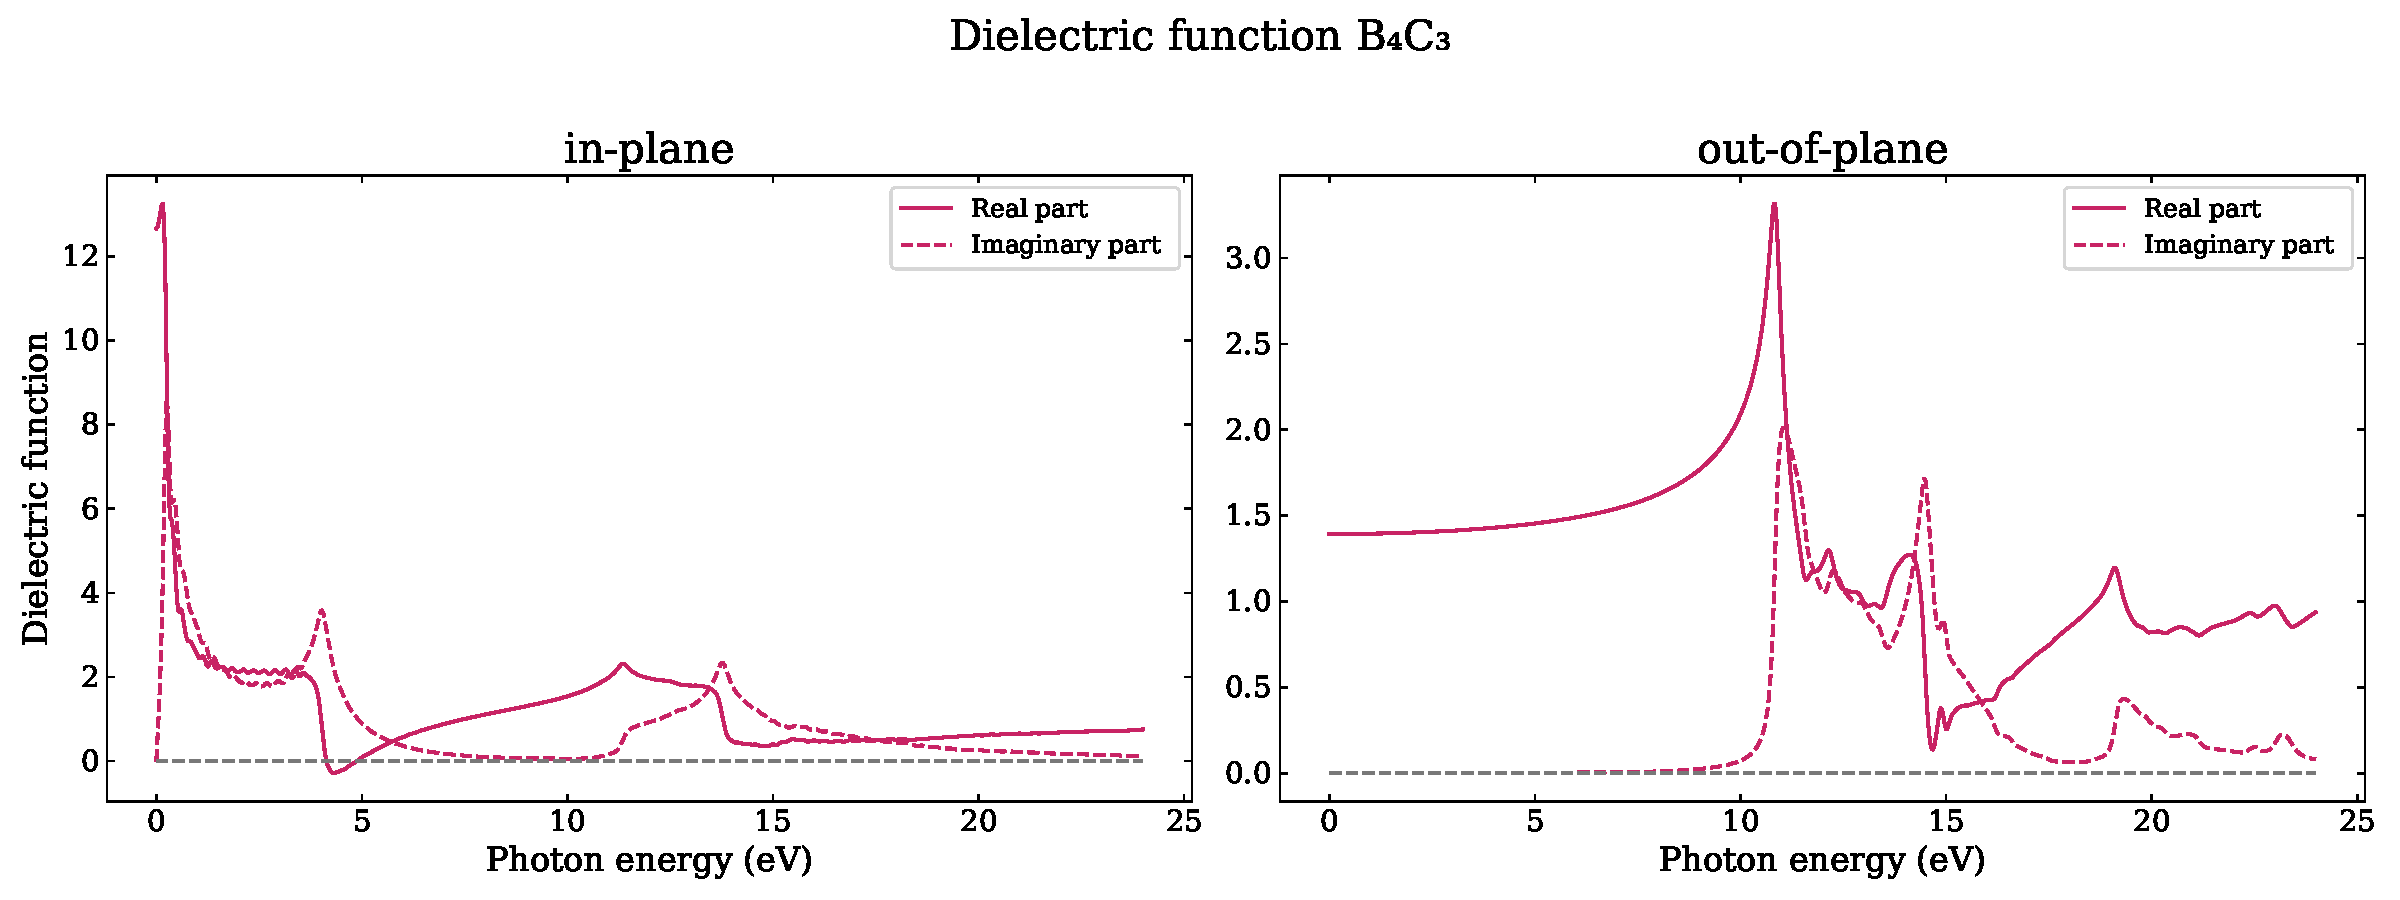
\includegraphics[width=0.80\linewidth]{figures_proj1/S1.13d.pdf}
\caption{Real and imaginary part of the dielectric function
for all the four monolayers as calculated using the PBE functional with a 
$129\times 129\times 129$
$\vec{k}$-point mesh for Graphene and a
$65\times 65 \times 65$
$\vec{k}$-point mesh for the borophene and boron-carbide monolayers.}
\label{S1.13}
\end{figure}

\begin{figure}[!htbp]
    \centering
    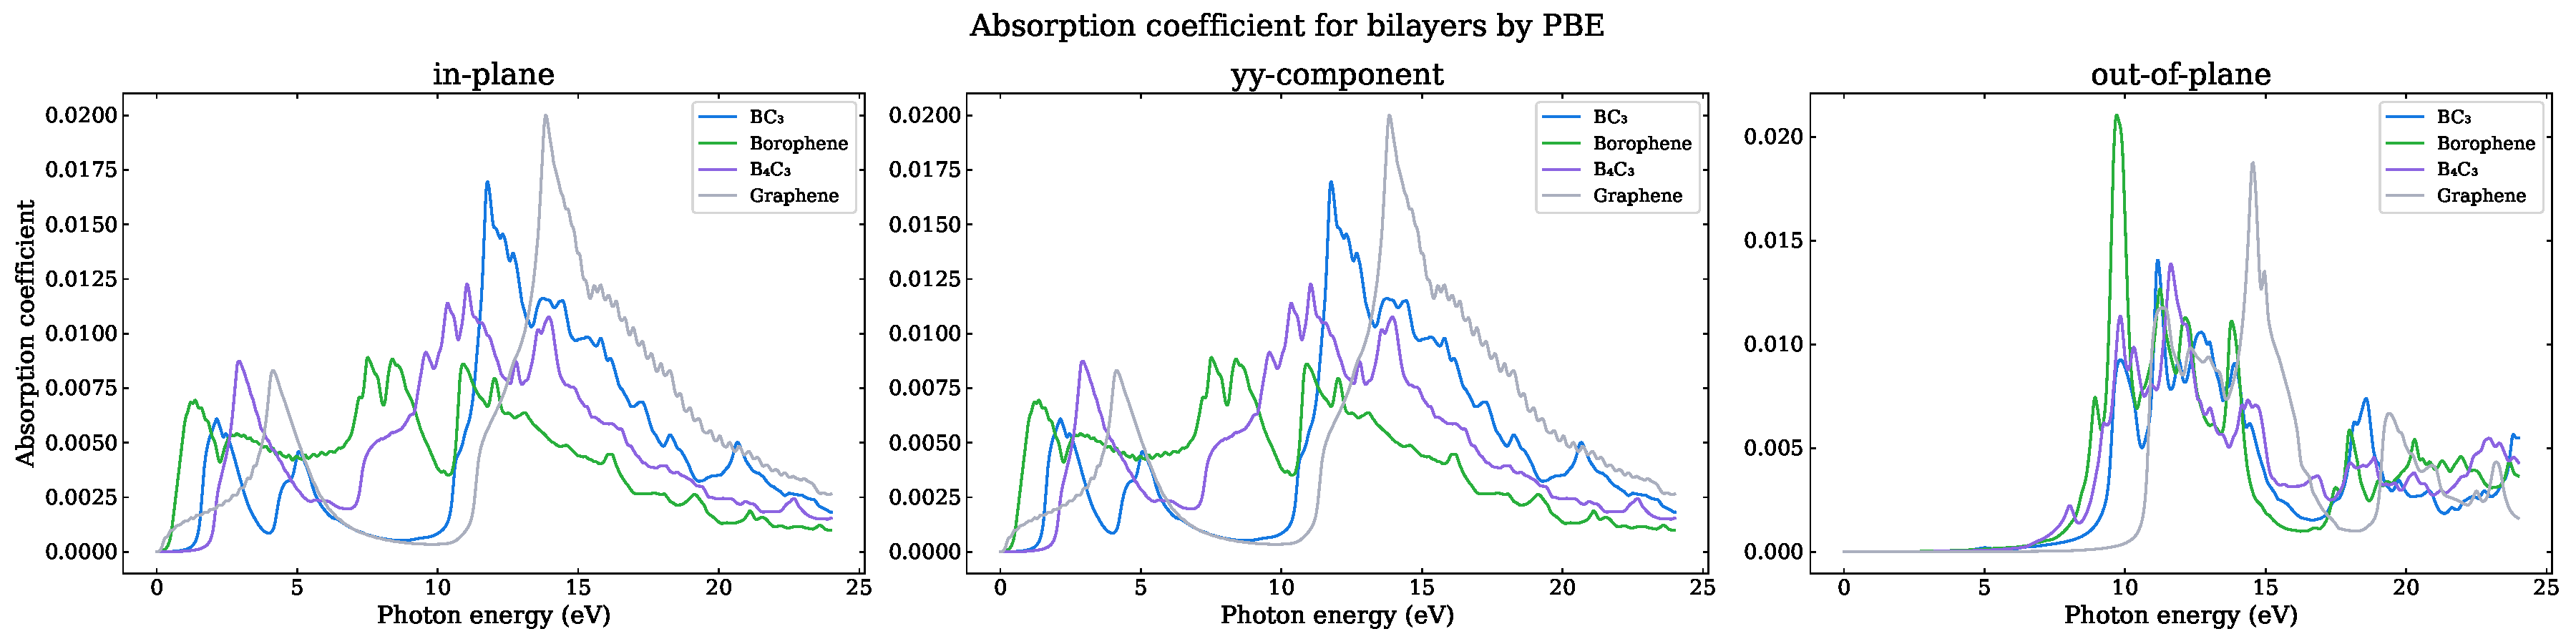
\includegraphics[width=0.80\linewidth]{figures_proj1/S1.14a.pdf}
    \par\nointerlineskip
    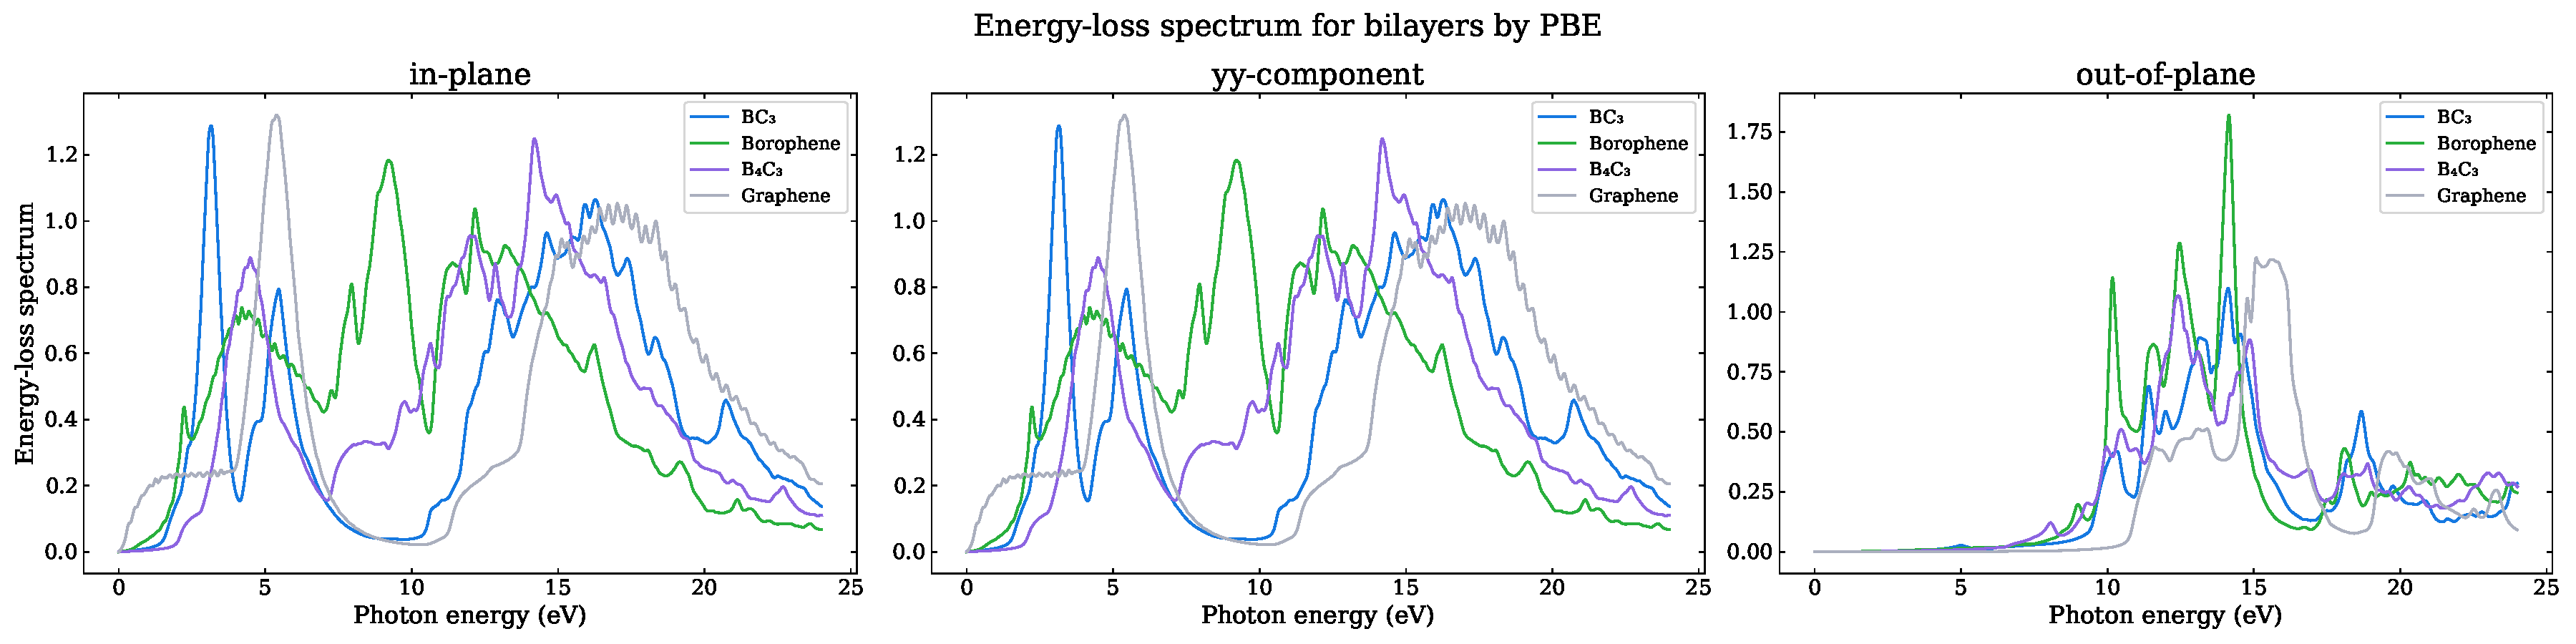
\includegraphics[width=0.80\linewidth]{figures_proj1/S1.14b.pdf}
    \par\nointerlineskip
    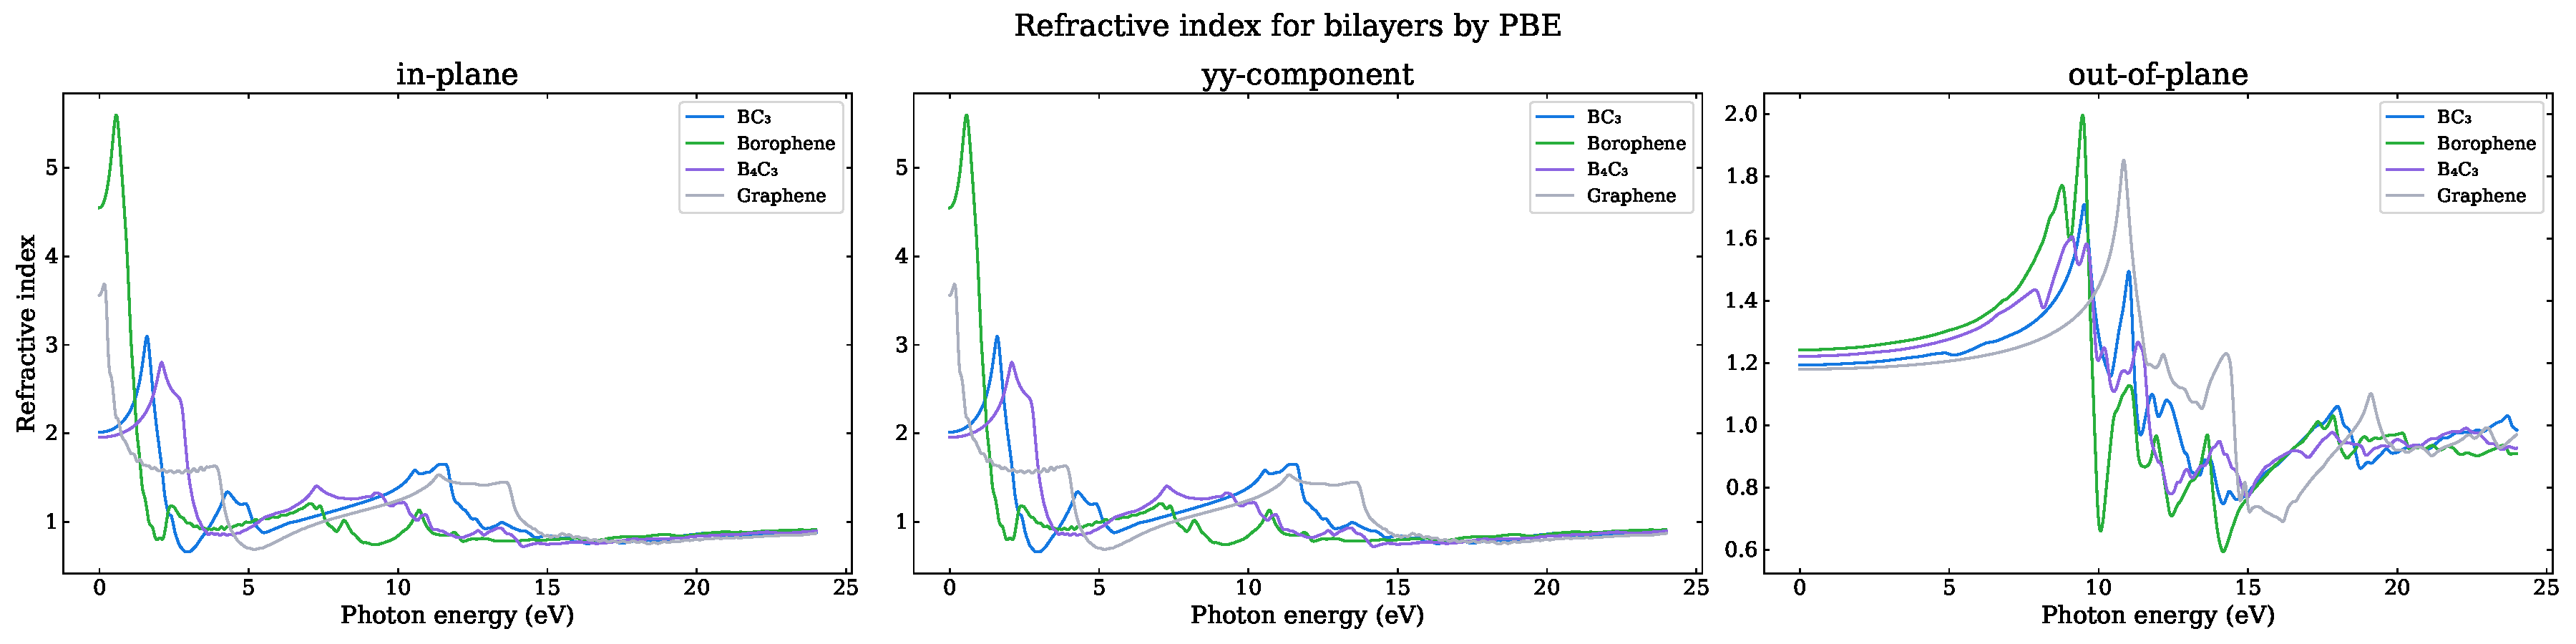
\includegraphics[width=0.80\linewidth]{figures_proj1/S1.14c.pdf}
    \par\nointerlineskip
    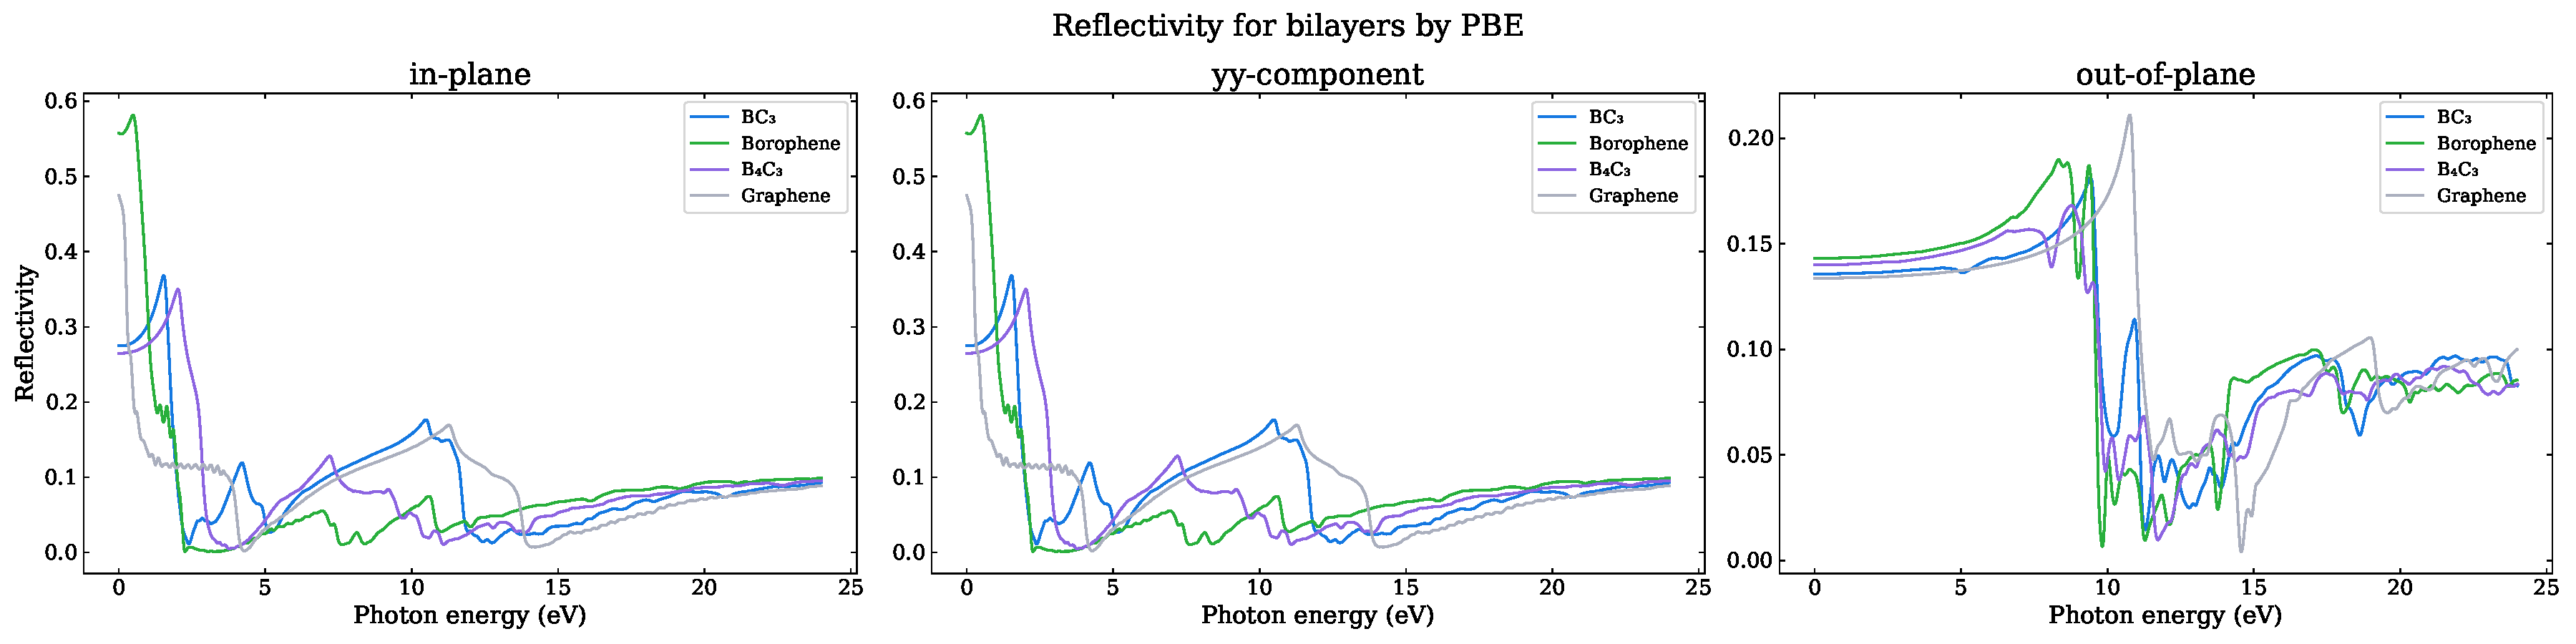
\includegraphics[width=0.80\linewidth]{figures_proj1/S1.14d.pdf}
    \par\nointerlineskip
    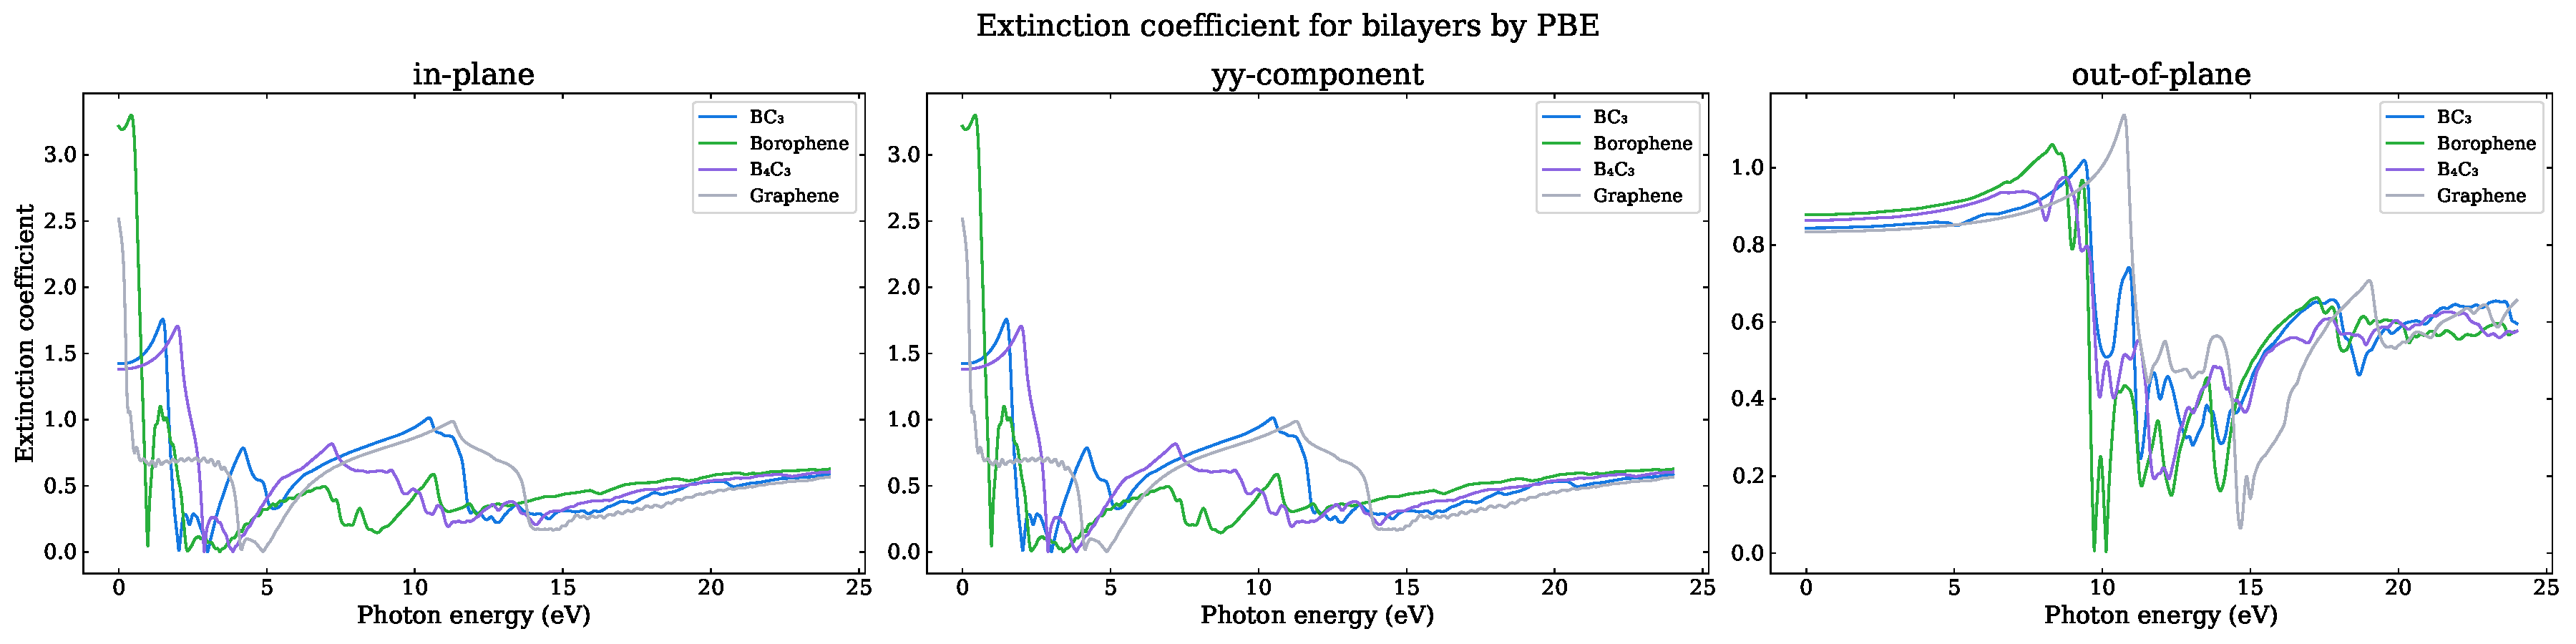
\includegraphics[width=0.80\linewidth]{figures_proj1/S1.14e.pdf}
\caption{Optical properties
for all the four monolayers as calculated using the PBE functional with a 
$129\times 129\times 129$
$\vec{k}$-point mesh for Graphene and a
$65\times 65 \times 65$
$\vec{k}$-point mesh for the borophene and boron-carbide monolayers.}
\label{S1.14}
\end{figure}

\begin{figure}[!htbp]
\centering
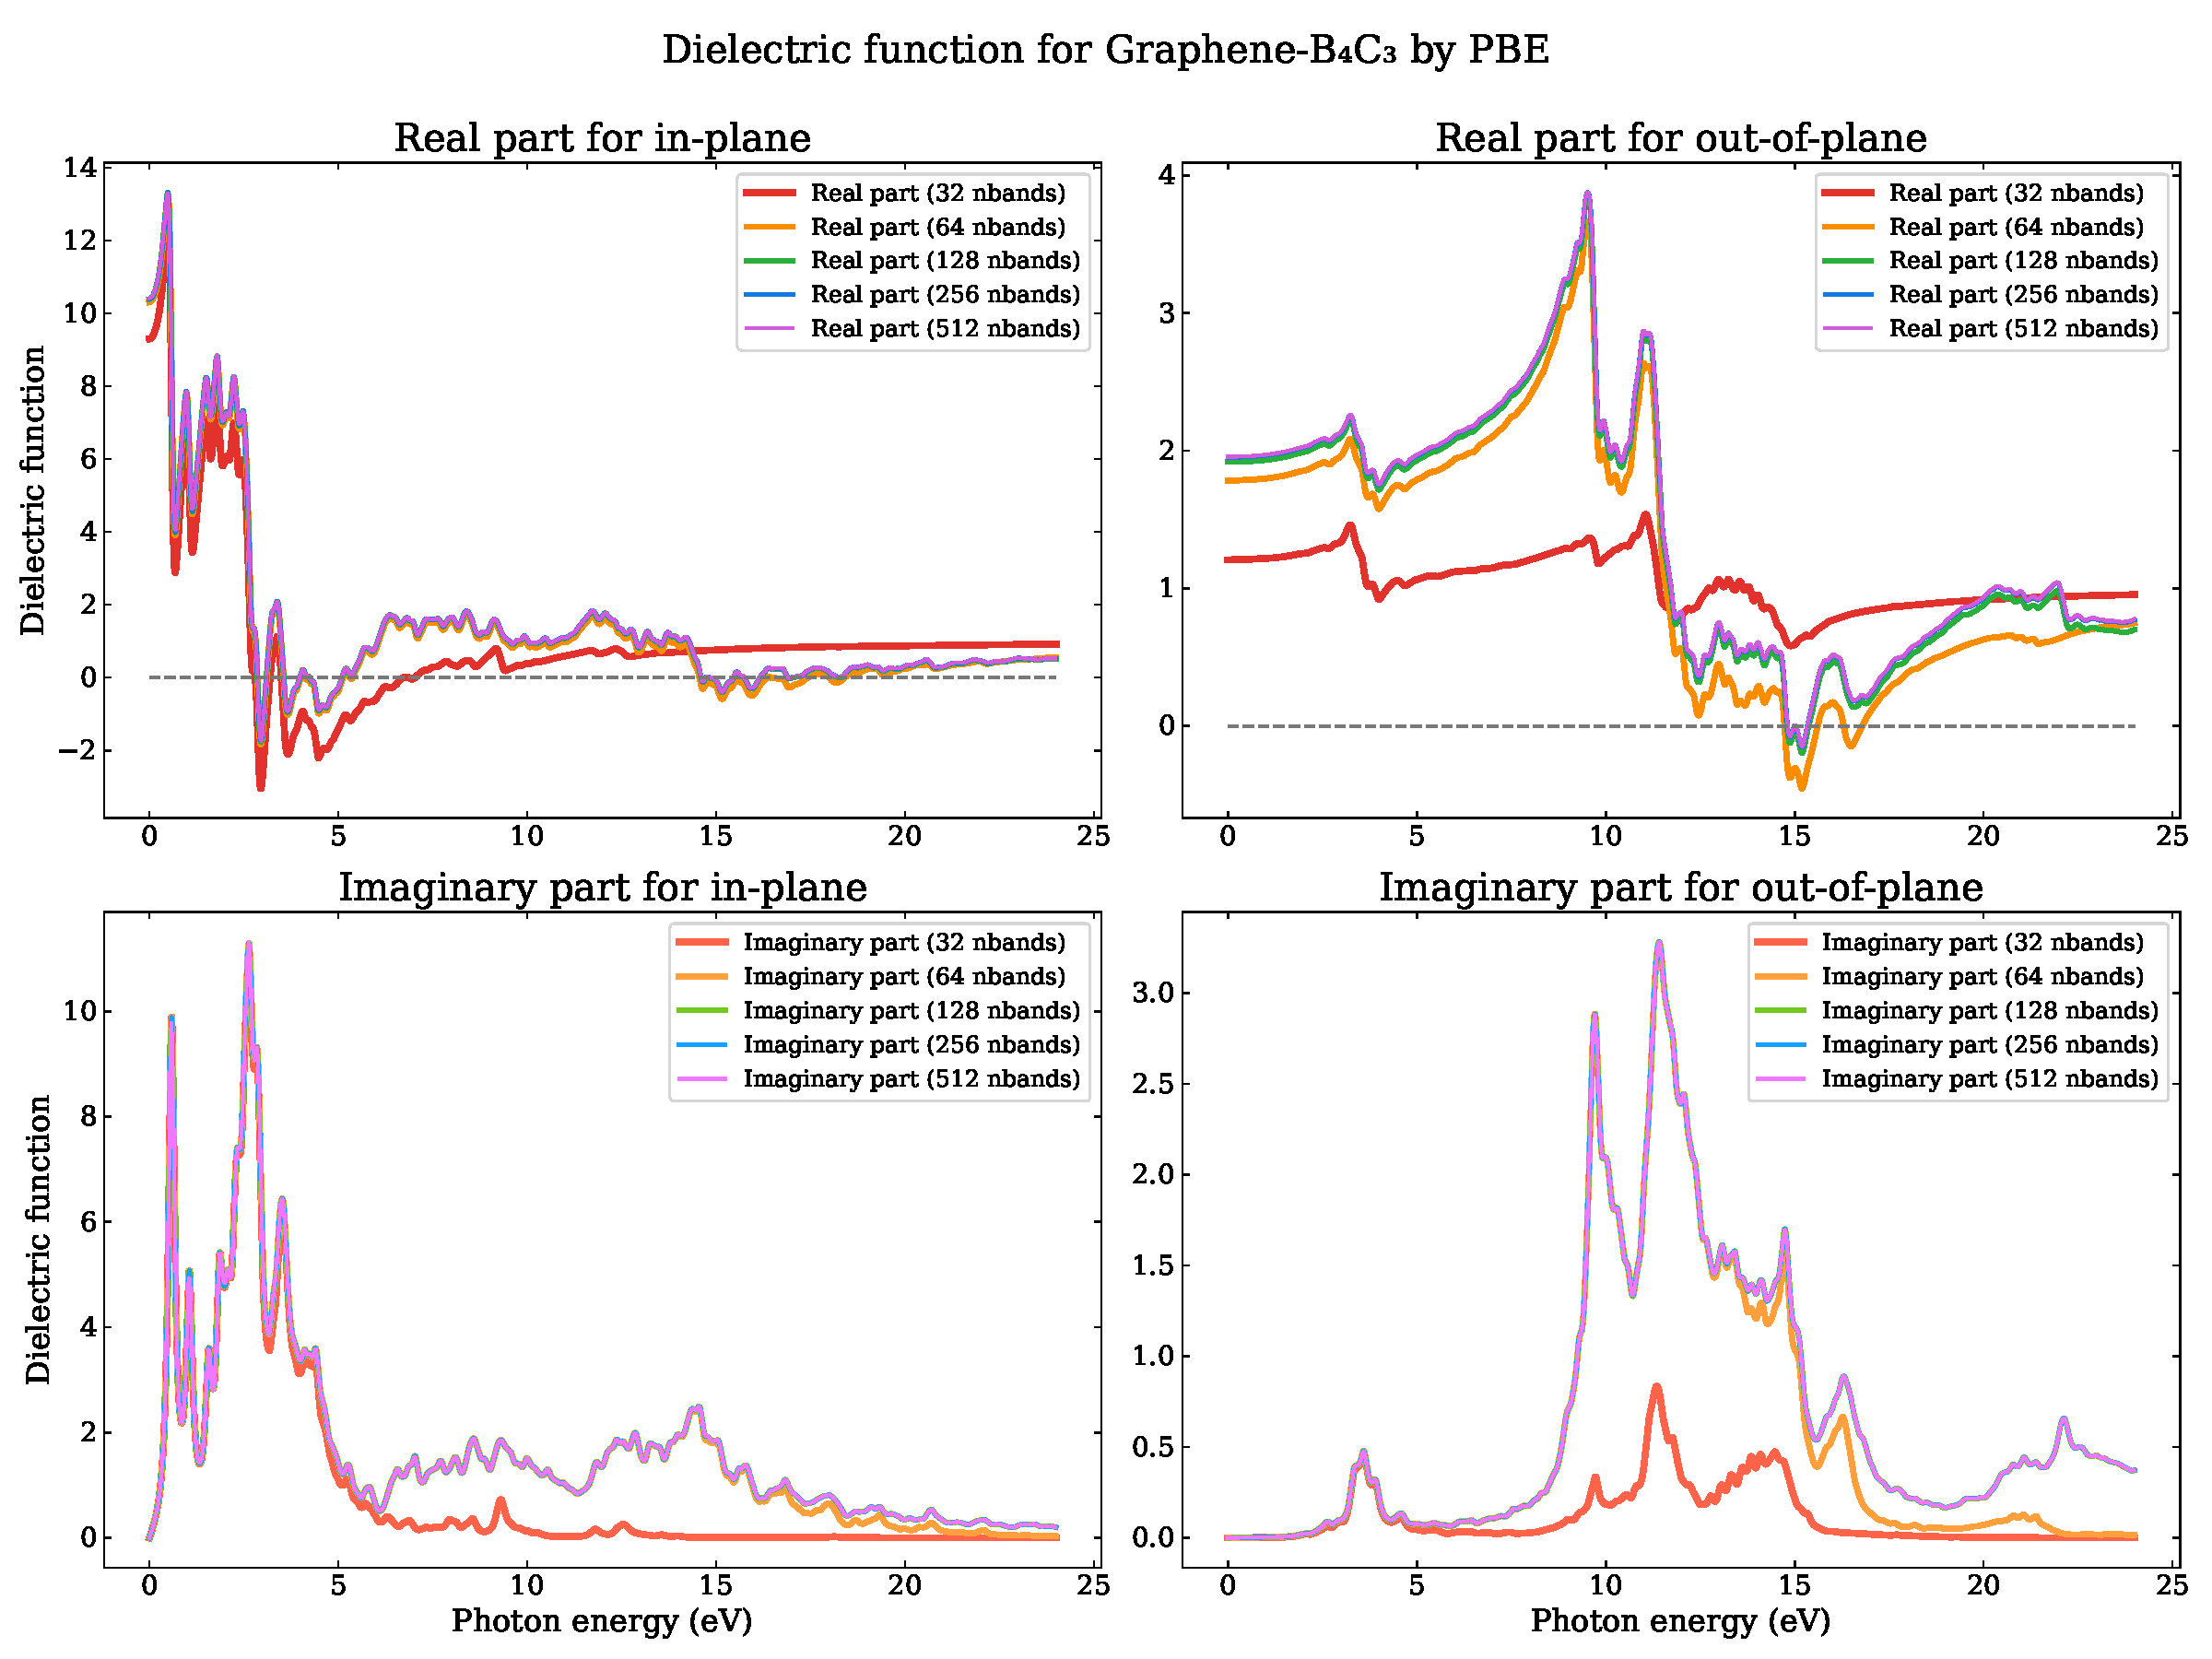
\includegraphics[width=0.80\textwidth]{figures_proj1/S1.15.pdf}
\caption{Convergence test for the number of unoccupied bands in calculating the dielectric function of the \ce{Graphene-B4C3} bilayer as calculated using the PBE functional.}
\label{S1.15}
\end{figure}

\clearpage We also test the effect of the energy convergence criteria ``EDIFF'' on the calculated dielectric function in figure~\ref{S1.16} along with different $\vec{k}$-point meshes and comparison of HSE06 and PBE.

\begin{figure}[!htbp]
\centering
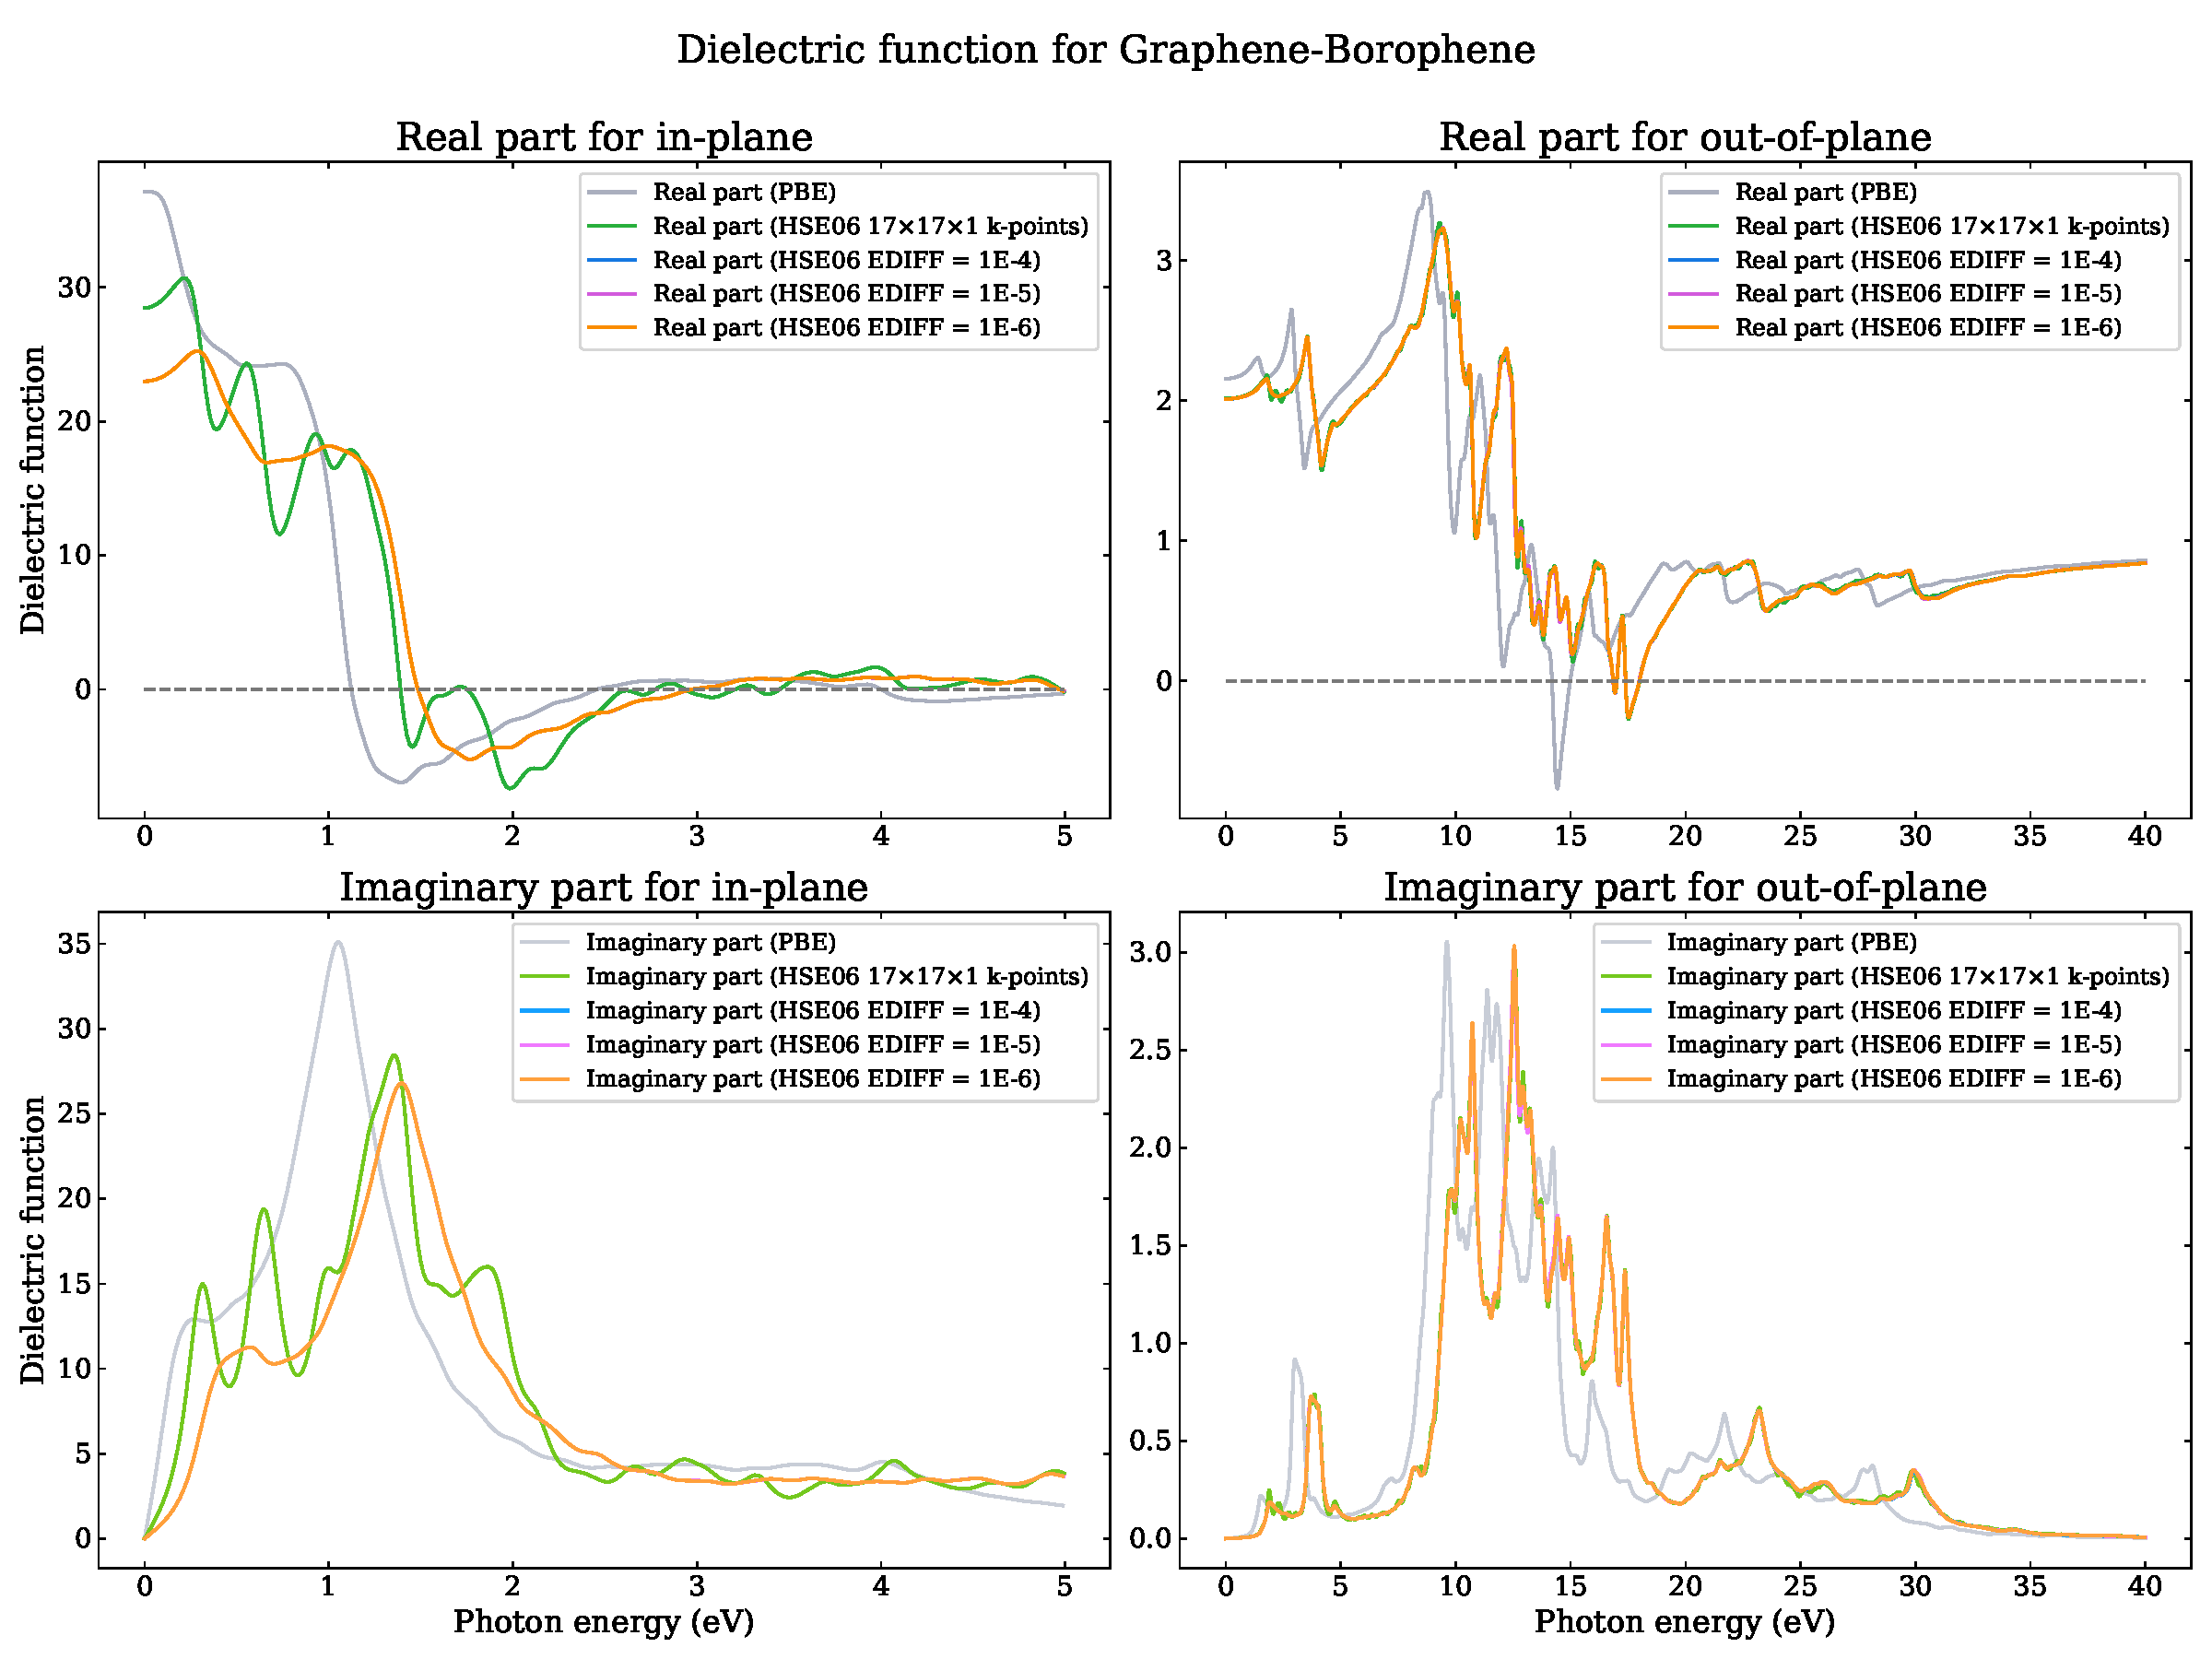
\includegraphics[width=0.80\textwidth]{figures_proj1/S1.16.pdf}
\caption{Dielectric function of the \ce{Graphene-Borophene} bilayer comparing HSE06 results obtained using $17 \times 17 \times 1$ and $65 \times 65 \times 1$ $\vec{k}$-point meshes,
with the PBE result included for reference.}
\label{S1.16}
\end{figure}

\clearpage
\begin{figure}[!htbp]
\centering
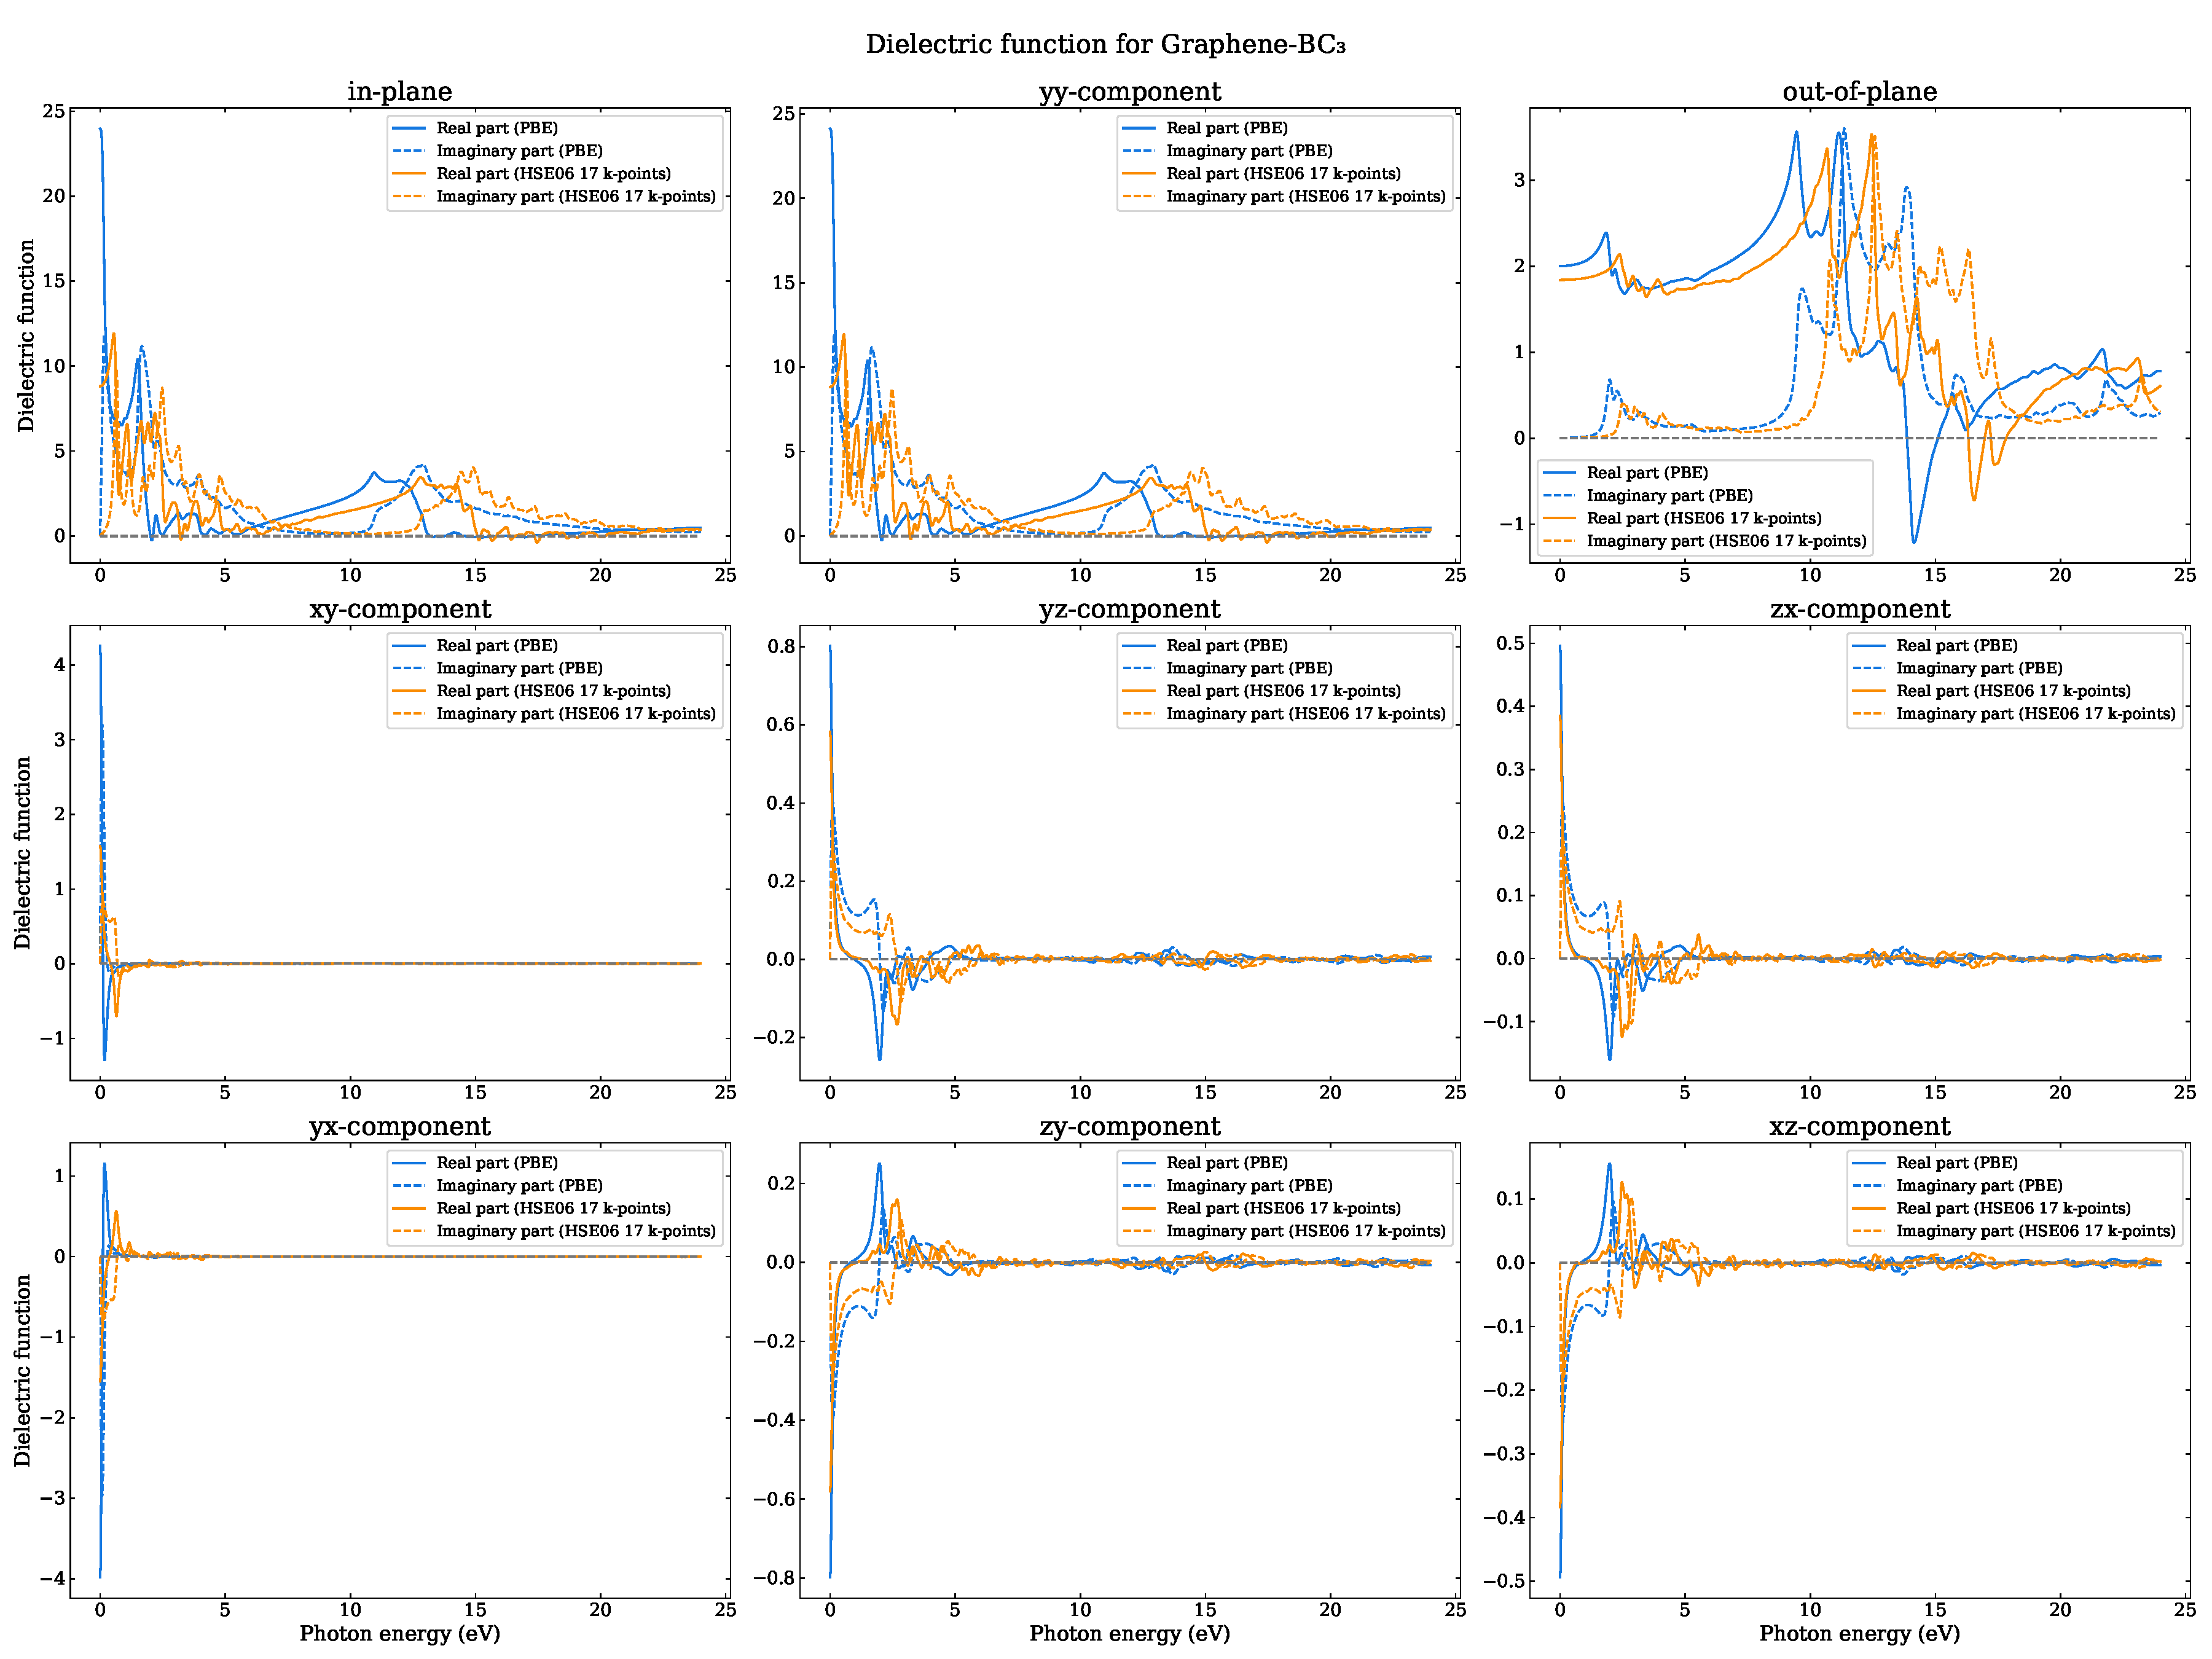
\includegraphics[width=0.80\textwidth]{figures_proj1/S1.17.pdf}
\caption{The components of the dielectric function of the \ce{Graphene-BC3} bilayer as calculated using the PBE functional displaying the small, non-zero values of the off-diagonal elements,
and the relationship: $yx=-xy$, $yz=-zy$, and $zx=-xz$}
\label{S1.17}
\end{figure}

\begin{figure}[!htbp]
\centering
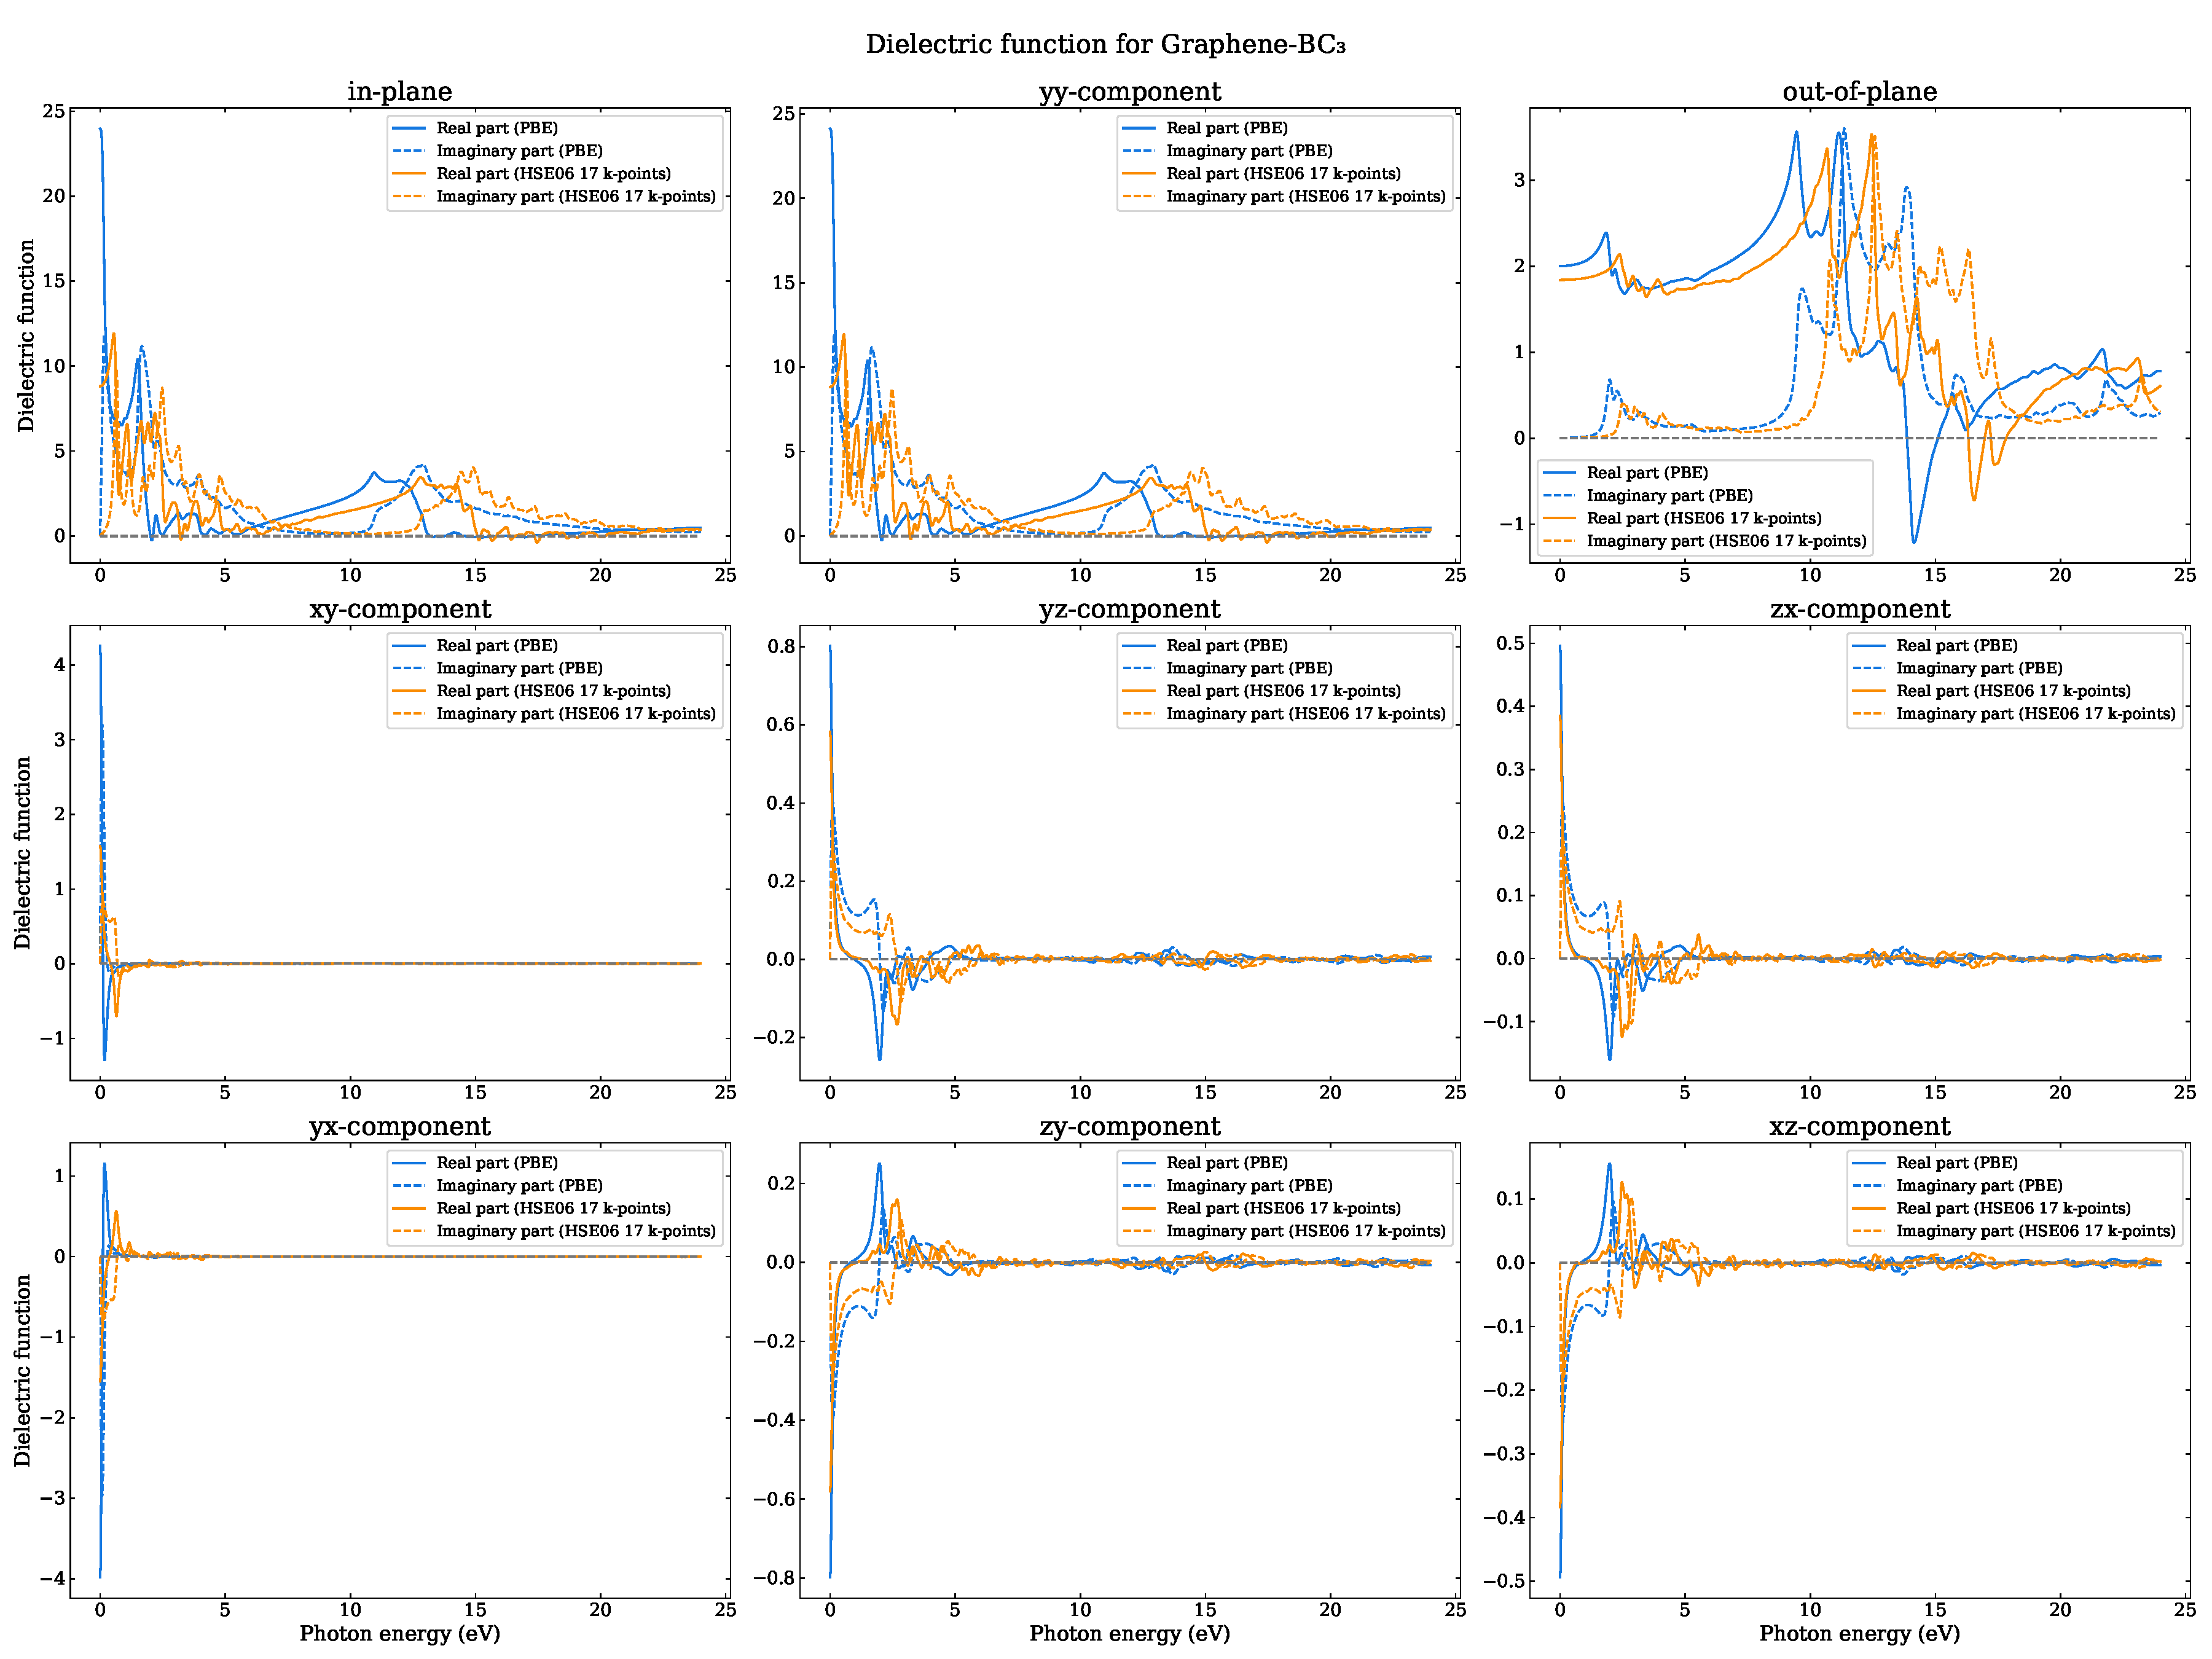
\includegraphics[width=0.80\textwidth]{figures_proj1/S1.18.pdf}
\caption{The components of the dielectric function of the \ce{Graphene-Borophene} bilayer as calculated using the PBE functional displaying the small, non-zero values of the off-diagonal elements,
and the relationship: $yx=-xy$, $yz=-zy$, and $zx=-xz$}
\label{S1.18}
\end{figure}

\begin{figure}[!htbp]
\centering
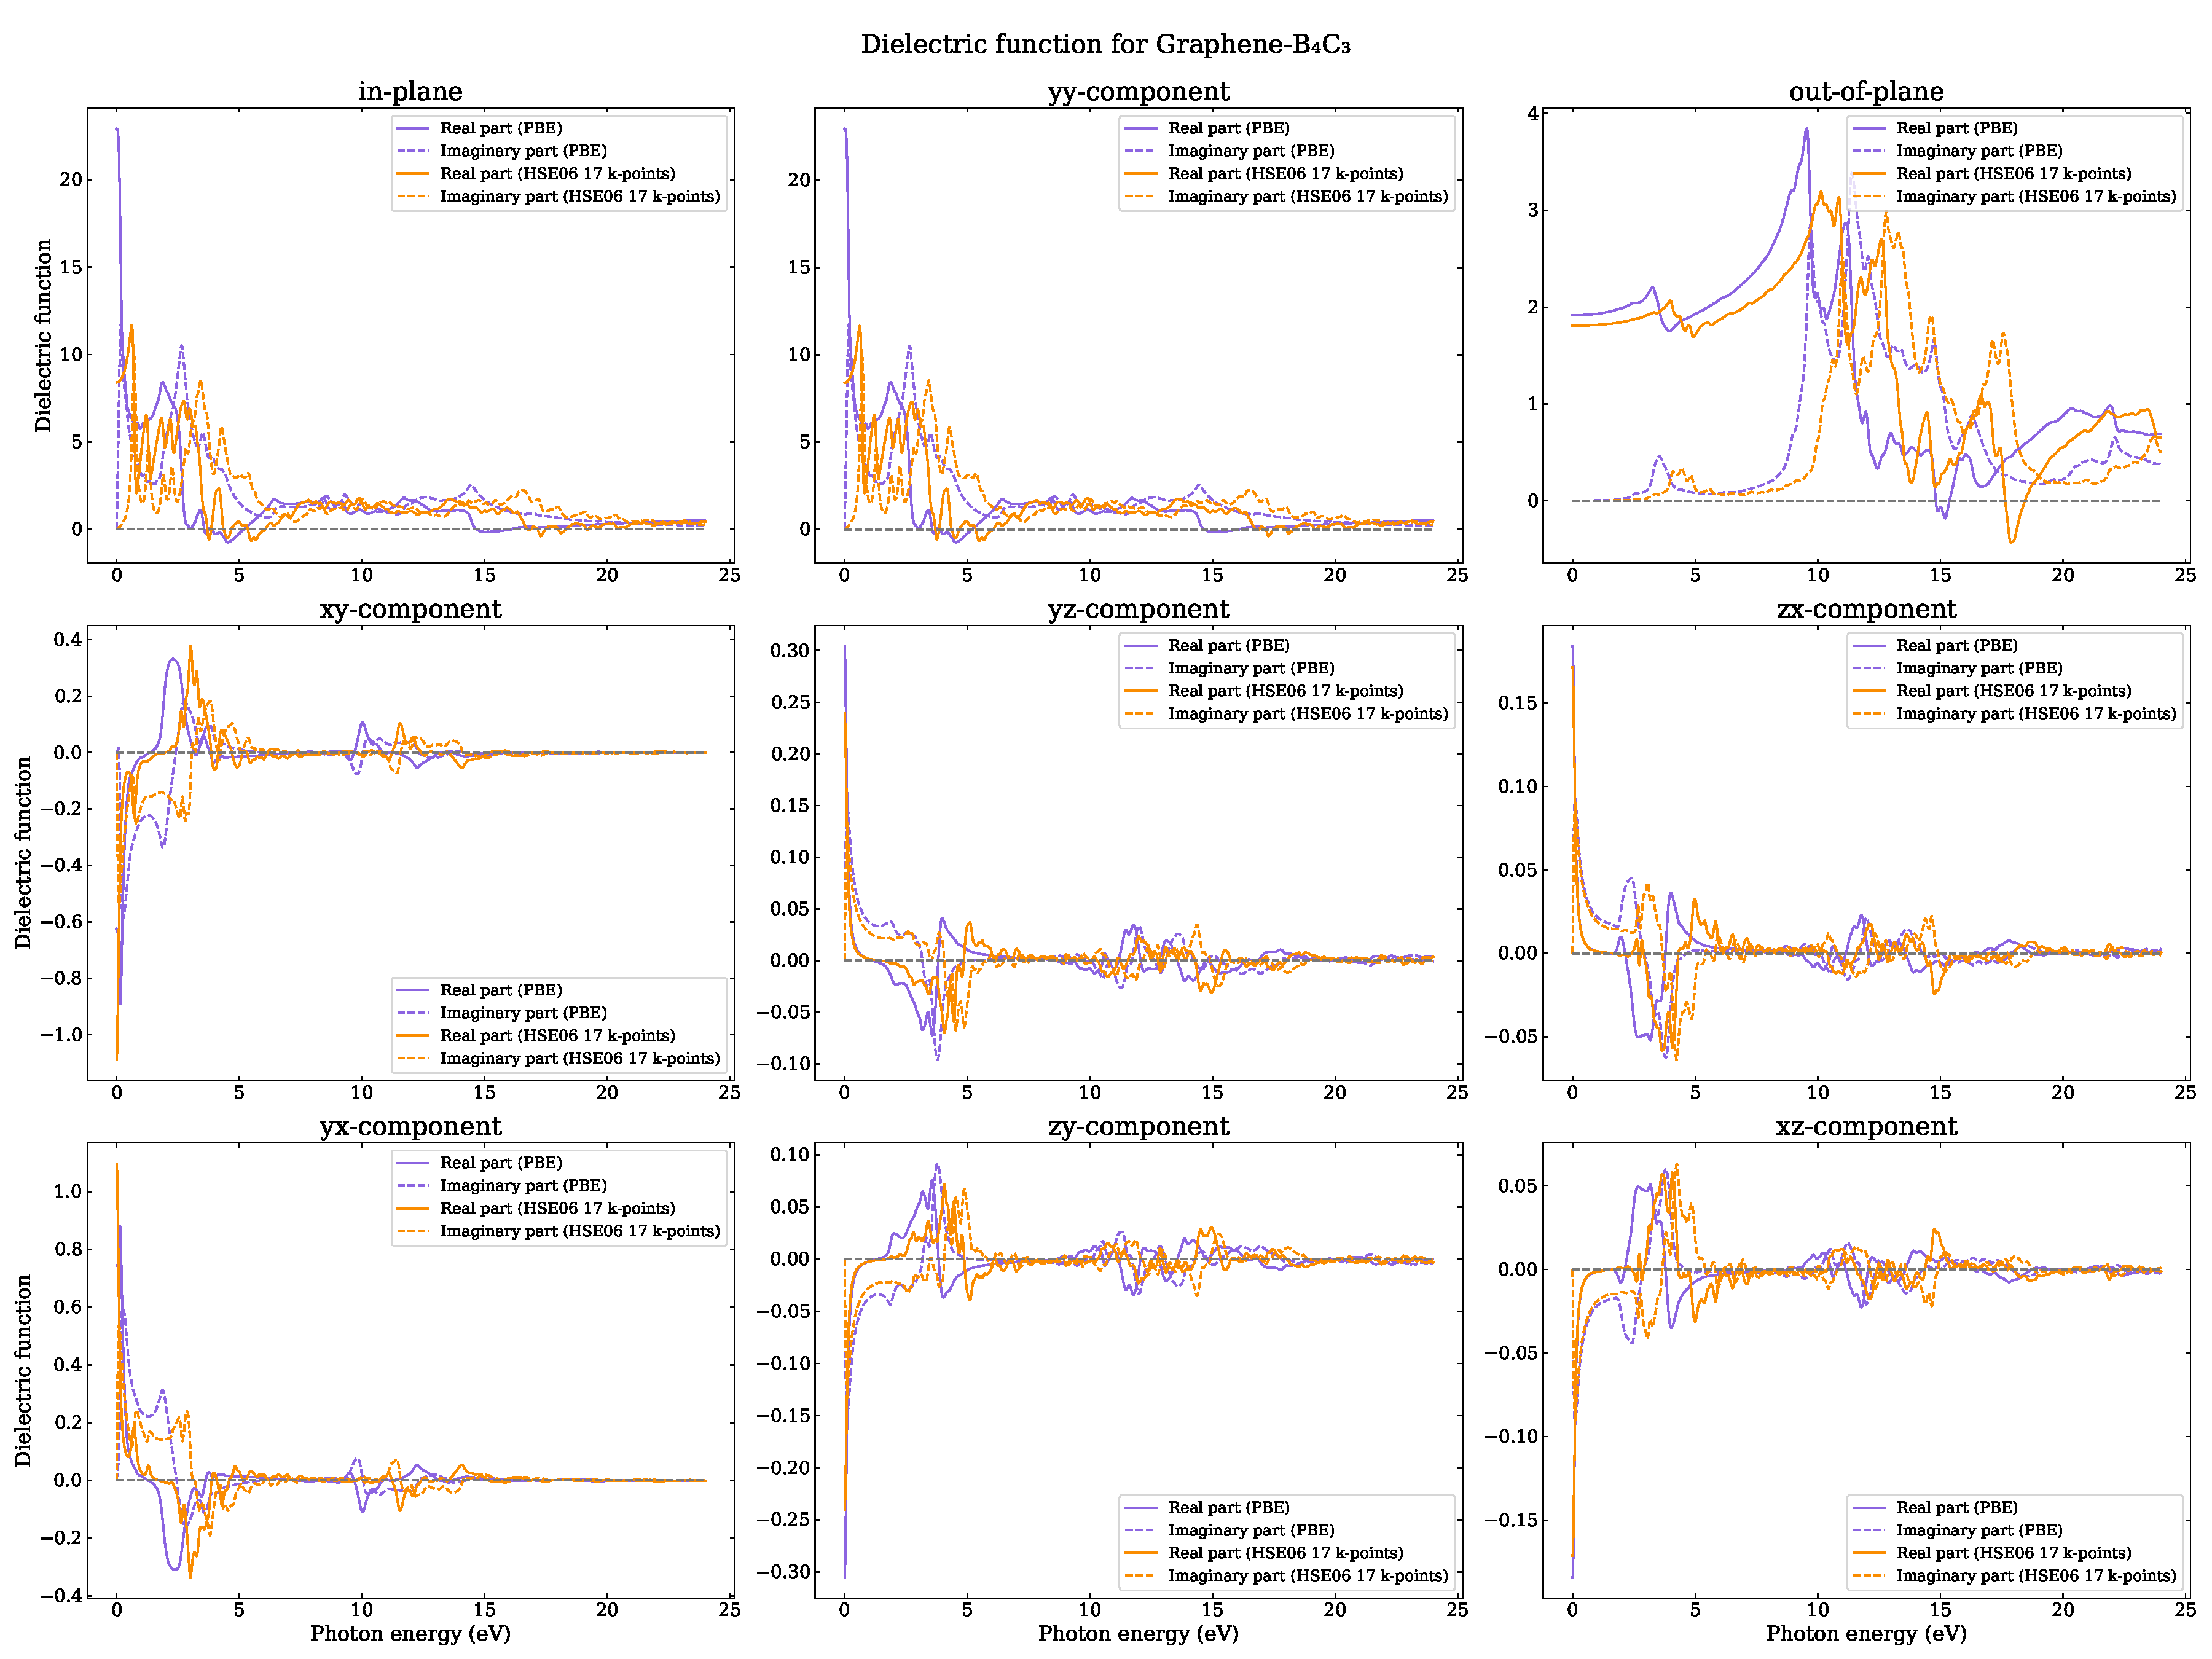
\includegraphics[width=0.80\textwidth]{figures_proj1/S1.19.pdf}
\caption{The components of the dielectric function of the \ce{Graphene-B4C3} bilayer as calculated using the PBE functional displaying the small, non-zero values of the off-diagonal elements,
and the relationship: $yx=-xy$, $yz=-zy$, and $zx=-xz$}
\label{S1.19}
\end{figure}

% test test test test
% no S7, S8
% S19-23 to S20-24
% line 82;
% line 247, 250;
% line 368, 370;
